% Options for packages loaded elsewhere
% Options for packages loaded elsewhere
\PassOptionsToPackage{unicode}{hyperref}
\PassOptionsToPackage{hyphens}{url}
\PassOptionsToPackage{dvipsnames,svgnames,x11names}{xcolor}
%
\documentclass[
  letterpaper,
  DIV=11,
  numbers=noendperiod]{scrartcl}
\usepackage{xcolor}
\usepackage[top=30mm,left=30mm]{geometry}
\usepackage{amsmath,amssymb}
\setcounter{secnumdepth}{-\maxdimen} % remove section numbering
\usepackage{iftex}
\ifPDFTeX
  \usepackage[T1]{fontenc}
  \usepackage[utf8]{inputenc}
  \usepackage{textcomp} % provide euro and other symbols
\else % if luatex or xetex
  \usepackage{unicode-math} % this also loads fontspec
  \defaultfontfeatures{Scale=MatchLowercase}
  \defaultfontfeatures[\rmfamily]{Ligatures=TeX,Scale=1}
\fi
\usepackage{lmodern}
\ifPDFTeX\else
  % xetex/luatex font selection
\fi
% Use upquote if available, for straight quotes in verbatim environments
\IfFileExists{upquote.sty}{\usepackage{upquote}}{}
\IfFileExists{microtype.sty}{% use microtype if available
  \usepackage[]{microtype}
  \UseMicrotypeSet[protrusion]{basicmath} % disable protrusion for tt fonts
}{}
\makeatletter
\@ifundefined{KOMAClassName}{% if non-KOMA class
  \IfFileExists{parskip.sty}{%
    \usepackage{parskip}
  }{% else
    \setlength{\parindent}{0pt}
    \setlength{\parskip}{6pt plus 2pt minus 1pt}}
}{% if KOMA class
  \KOMAoptions{parskip=half}}
\makeatother
% Make \paragraph and \subparagraph free-standing
\makeatletter
\ifx\paragraph\undefined\else
  \let\oldparagraph\paragraph
  \renewcommand{\paragraph}{
    \@ifstar
      \xxxParagraphStar
      \xxxParagraphNoStar
  }
  \newcommand{\xxxParagraphStar}[1]{\oldparagraph*{#1}\mbox{}}
  \newcommand{\xxxParagraphNoStar}[1]{\oldparagraph{#1}\mbox{}}
\fi
\ifx\subparagraph\undefined\else
  \let\oldsubparagraph\subparagraph
  \renewcommand{\subparagraph}{
    \@ifstar
      \xxxSubParagraphStar
      \xxxSubParagraphNoStar
  }
  \newcommand{\xxxSubParagraphStar}[1]{\oldsubparagraph*{#1}\mbox{}}
  \newcommand{\xxxSubParagraphNoStar}[1]{\oldsubparagraph{#1}\mbox{}}
\fi
\makeatother

\usepackage{color}
\usepackage{fancyvrb}
\newcommand{\VerbBar}{|}
\newcommand{\VERB}{\Verb[commandchars=\\\{\}]}
\DefineVerbatimEnvironment{Highlighting}{Verbatim}{commandchars=\\\{\}}
% Add ',fontsize=\small' for more characters per line
\usepackage{framed}
\definecolor{shadecolor}{RGB}{241,243,245}
\newenvironment{Shaded}{\begin{snugshade}}{\end{snugshade}}
\newcommand{\AlertTok}[1]{\textcolor[rgb]{0.68,0.00,0.00}{#1}}
\newcommand{\AnnotationTok}[1]{\textcolor[rgb]{0.37,0.37,0.37}{#1}}
\newcommand{\AttributeTok}[1]{\textcolor[rgb]{0.40,0.45,0.13}{#1}}
\newcommand{\BaseNTok}[1]{\textcolor[rgb]{0.68,0.00,0.00}{#1}}
\newcommand{\BuiltInTok}[1]{\textcolor[rgb]{0.00,0.23,0.31}{#1}}
\newcommand{\CharTok}[1]{\textcolor[rgb]{0.13,0.47,0.30}{#1}}
\newcommand{\CommentTok}[1]{\textcolor[rgb]{0.37,0.37,0.37}{#1}}
\newcommand{\CommentVarTok}[1]{\textcolor[rgb]{0.37,0.37,0.37}{\textit{#1}}}
\newcommand{\ConstantTok}[1]{\textcolor[rgb]{0.56,0.35,0.01}{#1}}
\newcommand{\ControlFlowTok}[1]{\textcolor[rgb]{0.00,0.23,0.31}{\textbf{#1}}}
\newcommand{\DataTypeTok}[1]{\textcolor[rgb]{0.68,0.00,0.00}{#1}}
\newcommand{\DecValTok}[1]{\textcolor[rgb]{0.68,0.00,0.00}{#1}}
\newcommand{\DocumentationTok}[1]{\textcolor[rgb]{0.37,0.37,0.37}{\textit{#1}}}
\newcommand{\ErrorTok}[1]{\textcolor[rgb]{0.68,0.00,0.00}{#1}}
\newcommand{\ExtensionTok}[1]{\textcolor[rgb]{0.00,0.23,0.31}{#1}}
\newcommand{\FloatTok}[1]{\textcolor[rgb]{0.68,0.00,0.00}{#1}}
\newcommand{\FunctionTok}[1]{\textcolor[rgb]{0.28,0.35,0.67}{#1}}
\newcommand{\ImportTok}[1]{\textcolor[rgb]{0.00,0.46,0.62}{#1}}
\newcommand{\InformationTok}[1]{\textcolor[rgb]{0.37,0.37,0.37}{#1}}
\newcommand{\KeywordTok}[1]{\textcolor[rgb]{0.00,0.23,0.31}{\textbf{#1}}}
\newcommand{\NormalTok}[1]{\textcolor[rgb]{0.00,0.23,0.31}{#1}}
\newcommand{\OperatorTok}[1]{\textcolor[rgb]{0.37,0.37,0.37}{#1}}
\newcommand{\OtherTok}[1]{\textcolor[rgb]{0.00,0.23,0.31}{#1}}
\newcommand{\PreprocessorTok}[1]{\textcolor[rgb]{0.68,0.00,0.00}{#1}}
\newcommand{\RegionMarkerTok}[1]{\textcolor[rgb]{0.00,0.23,0.31}{#1}}
\newcommand{\SpecialCharTok}[1]{\textcolor[rgb]{0.37,0.37,0.37}{#1}}
\newcommand{\SpecialStringTok}[1]{\textcolor[rgb]{0.13,0.47,0.30}{#1}}
\newcommand{\StringTok}[1]{\textcolor[rgb]{0.13,0.47,0.30}{#1}}
\newcommand{\VariableTok}[1]{\textcolor[rgb]{0.07,0.07,0.07}{#1}}
\newcommand{\VerbatimStringTok}[1]{\textcolor[rgb]{0.13,0.47,0.30}{#1}}
\newcommand{\WarningTok}[1]{\textcolor[rgb]{0.37,0.37,0.37}{\textit{#1}}}

\usepackage{longtable,booktabs,array}
\newcounter{none} % for unnumbered tables
\usepackage{calc} % for calculating minipage widths
% Correct order of tables after \paragraph or \subparagraph
\usepackage{etoolbox}
\makeatletter
\patchcmd\longtable{\par}{\if@noskipsec\mbox{}\fi\par}{}{}
\makeatother
% Allow footnotes in longtable head/foot
\IfFileExists{footnotehyper.sty}{\usepackage{footnotehyper}}{\usepackage{footnote}}
\makesavenoteenv{longtable}
\usepackage{graphicx}
\makeatletter
\newsavebox\pandoc@box
\newcommand*\pandocbounded[1]{% scales image to fit in text height/width
  \sbox\pandoc@box{#1}%
  \Gscale@div\@tempa{\textheight}{\dimexpr\ht\pandoc@box+\dp\pandoc@box\relax}%
  \Gscale@div\@tempb{\linewidth}{\wd\pandoc@box}%
  \ifdim\@tempb\p@<\@tempa\p@\let\@tempa\@tempb\fi% select the smaller of both
  \ifdim\@tempa\p@<\p@\scalebox{\@tempa}{\usebox\pandoc@box}%
  \else\usebox{\pandoc@box}%
  \fi%
}
% Set default figure placement to htbp
\def\fps@figure{htbp}
\makeatother


% definitions for citeproc citations
\NewDocumentCommand\citeproctext{}{}
\NewDocumentCommand\citeproc{mm}{%
  \begingroup\def\citeproctext{#2}\cite{#1}\endgroup}
\makeatletter
 % allow citations to break across lines
 \let\@cite@ofmt\@firstofone
 % avoid brackets around text for \cite:
 \def\@biblabel#1{}
 \def\@cite#1#2{{#1\if@tempswa , #2\fi}}
\makeatother
\newlength{\cslhangindent}
\setlength{\cslhangindent}{1.5em}
\newlength{\csllabelwidth}
\setlength{\csllabelwidth}{3em}
\newenvironment{CSLReferences}[2] % #1 hanging-indent, #2 entry-spacing
 {\begin{list}{}{%
  \setlength{\itemindent}{0pt}
  \setlength{\leftmargin}{0pt}
  \setlength{\parsep}{0pt}
  % turn on hanging indent if param 1 is 1
  \ifodd #1
   \setlength{\leftmargin}{\cslhangindent}
   \setlength{\itemindent}{-1\cslhangindent}
  \fi
  % set entry spacing
  \setlength{\itemsep}{#2\baselineskip}}}
 {\end{list}}
\usepackage{calc}
\newcommand{\CSLBlock}[1]{\hfill\break\parbox[t]{\linewidth}{\strut\ignorespaces#1\strut}}
\newcommand{\CSLLeftMargin}[1]{\parbox[t]{\csllabelwidth}{\strut#1\strut}}
\newcommand{\CSLRightInline}[1]{\parbox[t]{\linewidth - \csllabelwidth}{\strut#1\strut}}
\newcommand{\CSLIndent}[1]{\hspace{\cslhangindent}#1}



\setlength{\emergencystretch}{3em} % prevent overfull lines

\providecommand{\tightlist}{%
  \setlength{\itemsep}{0pt}\setlength{\parskip}{0pt}}



 


\KOMAoption{captions}{tableheading}
\makeatletter
\@ifpackageloaded{tcolorbox}{}{\usepackage[skins,breakable]{tcolorbox}}
\@ifpackageloaded{fontawesome5}{}{\usepackage{fontawesome5}}
\definecolor{quarto-callout-color}{HTML}{909090}
\definecolor{quarto-callout-note-color}{HTML}{0758E5}
\definecolor{quarto-callout-important-color}{HTML}{CC1914}
\definecolor{quarto-callout-warning-color}{HTML}{EB9113}
\definecolor{quarto-callout-tip-color}{HTML}{00A047}
\definecolor{quarto-callout-caution-color}{HTML}{FC5300}
\definecolor{quarto-callout-color-frame}{HTML}{acacac}
\definecolor{quarto-callout-note-color-frame}{HTML}{4582ec}
\definecolor{quarto-callout-important-color-frame}{HTML}{d9534f}
\definecolor{quarto-callout-warning-color-frame}{HTML}{f0ad4e}
\definecolor{quarto-callout-tip-color-frame}{HTML}{02b875}
\definecolor{quarto-callout-caution-color-frame}{HTML}{fd7e14}
\makeatother
\makeatletter
\@ifpackageloaded{caption}{}{\usepackage{caption}}
\AtBeginDocument{%
\ifdefined\contentsname
  \renewcommand*\contentsname{Table of contents}
\else
  \newcommand\contentsname{Table of contents}
\fi
\ifdefined\listfigurename
  \renewcommand*\listfigurename{List of Figures}
\else
  \newcommand\listfigurename{List of Figures}
\fi
\ifdefined\listtablename
  \renewcommand*\listtablename{List of Tables}
\else
  \newcommand\listtablename{List of Tables}
\fi
\ifdefined\figurename
  \renewcommand*\figurename{Figure}
\else
  \newcommand\figurename{Figure}
\fi
\ifdefined\tablename
  \renewcommand*\tablename{Table}
\else
  \newcommand\tablename{Table}
\fi
}
\@ifpackageloaded{float}{}{\usepackage{float}}
\floatstyle{ruled}
\@ifundefined{c@chapter}{\newfloat{codelisting}{h}{lop}}{\newfloat{codelisting}{h}{lop}[chapter]}
\floatname{codelisting}{Listing}
\newcommand*\listoflistings{\listof{codelisting}{List of Listings}}
\makeatother
\makeatletter
\makeatother
\makeatletter
\@ifpackageloaded{caption}{}{\usepackage{caption}}
\@ifpackageloaded{subcaption}{}{\usepackage{subcaption}}
\makeatother
\usepackage{bookmark}
\IfFileExists{xurl.sty}{\usepackage{xurl}}{} % add URL line breaks if available
\urlstyle{same}
\hypersetup{
  pdftitle={Predictive SSF Walkthrough},
  pdfauthor={Scott Forrest},
  colorlinks=true,
  linkcolor={blue},
  filecolor={Maroon},
  citecolor={Blue},
  urlcolor={Blue},
  pdfcreator={LaTeX via pandoc}}


\title{Predictive SSF Walkthrough}
\author{Scott Forrest}
\date{2026-08-25}
\begin{document}
\maketitle
\begin{abstract}
An end-to-end walkthrough of predictive movement ecology using step
selection functions. We fit two step selection functions to a single
water buffalo --- a \emph{static} model with constant selection
coefficients, and a \emph{temporally dynamic} GAM in which selection for
each covariate varies smoothly across the day --- and then use each
fitted model to generate stochastic movement trajectories. Those
simulations are aggregated into utilisation distributions, summarised
into hourly movement and habitat-use statistics, and validated against
the observed data. The aim is to show the full path from fitted
coefficients to spatial predictions, and to check whether the extra
flexibility of the dynamic model actually buys better predictions.
\end{abstract}

\renewcommand*\contentsname{Table of contents}
{
\setcounter{tocdepth}{3}
\tableofcontents
}

\section{Introduction}\label{introduction}

A step selection function (SSF) is usually the \emph{end} of an
analysis: we fit the model, report the coefficients, and interpret which
habitats an animal selected for. But a fitted SSF is also a complete,
generative description of a movement process. If we can fit it, we can
\emph{simulate} from it --- and simulated trajectories can be turned
into spatial predictions that we can validate.

This walkthrough takes that full path:

\begin{verbatim}
fit  ->  simulate  ->  aggregate  ->  hourly summaries  ->  assess predictions
\end{verbatim}

It is a simplified version of the analysis in Forrest et al. (2025),
whose full code lives at
\href{https://github.com/swforrest/dynamic_SSF_sims}{github.com/swforrest/dynamic\_SSF\_sims}.
Where that repository spreads the work across six scripts and a
high-performance computing cluster, here we compress it into one script
that runs on a laptop.

Throughout, we fit \textbf{two} models and carry both all the way to the
end:

{\def\LTcaptype{none} % do not increment counter
\begin{longtable}[]{@{}
  >{\raggedright\arraybackslash}p{(\linewidth - 2\tabcolsep) * \real{0.5000}}
  >{\raggedright\arraybackslash}p{(\linewidth - 2\tabcolsep) * \real{0.5000}}@{}}
\toprule\noalign{}
\endhead
\bottomrule\noalign{}
\endlastfoot
\textbf{Model A --- static} & An ordinary integrated SSF (iSSF). One
selection coefficient per covariate, constant across the day. \\
\textbf{Model B --- temporally dynamic} & A GAM in which each
coefficient is a smooth, cyclic function of the hour of day. \\
\end{longtable}
}

Carrying both through is the point. It is easy to show that a more
flexible model produces more interesting-looking coefficients. It is
much more informative to ask whether those coefficients translate into
\emph{better predictions} --- and that requires simulating, aggregating
and validating.

\section{Setup}\label{setup}

\subsection{Load required packages}\label{load-required-packages}

\begin{Shaded}
\begin{Highlighting}[]
\FunctionTok{library}\NormalTok{(tidyverse)}
\NormalTok{packages }\OtherTok{\textless{}{-}} \FunctionTok{c}\NormalTok{(}\StringTok{"amt"}\NormalTok{, }\StringTok{"sf"}\NormalTok{, }\StringTok{"terra"}\NormalTok{, }\StringTok{"mgcv"}\NormalTok{, }\StringTok{"gratia"}\NormalTok{, }\StringTok{"lubridate"}\NormalTok{,}
              \StringTok{"RColorBrewer"}\NormalTok{, }\StringTok{"viridis"}\NormalTok{, }\StringTok{"patchwork"}\NormalTok{, }\StringTok{"tictoc"}\NormalTok{, }\StringTok{"magick"}\NormalTok{)}
\FunctionTok{walk}\NormalTok{(packages, require, }\AttributeTok{character.only =} \ConstantTok{TRUE}\NormalTok{)}

\CommentTok{\# Two packages are deliberately NOT attached, and are called with \textasciigrave{}::\textasciigrave{} instead:}
\CommentTok{\#}
\CommentTok{\#  {-} \textasciigrave{}circular\textasciigrave{}, for the von Mises distribution. Attaching it would mask}
\CommentTok{\#    \textasciigrave{}stats::sd\textasciigrave{} and \textasciigrave{}stats::var\textasciigrave{}, which is an easy trap to fall into later.}
\CommentTok{\#  {-} \textasciigrave{}ecospat\textasciigrave{}, used once for the Boyce index; it pulls in a large dependency tree.}

\FunctionTok{options}\NormalTok{(}\AttributeTok{scipen =} \DecValTok{999}\NormalTok{)}
\end{Highlighting}
\end{Shaded}

\subsection{Parameters}\label{parameters}

Every quantity that controls the size or behaviour of the analysis lives
here, so the whole walkthrough can be re-run at a different scale
without hunting through the script. The defaults are chosen to run in a
reasonable time on a laptop; the comments indicate what to increase for
publication-quality results.

\begin{Shaded}
\begin{Highlighting}[]
\FunctionTok{set.seed}\NormalTok{(}\DecValTok{2158}\NormalTok{)}

\CommentTok{\# {-}{-}{-} Data selection {-}{-}{-}{-}{-}{-}{-}{-}{-}{-}{-}{-}{-}{-}{-}{-}{-}{-}{-}{-}{-}{-}{-}{-}{-}{-}{-}{-}{-}{-}{-}{-}{-}{-}{-}{-}{-}{-}{-}{-}{-}{-}{-}{-}{-}{-}{-}{-}{-}{-}{-}{-}{-}{-}}
\NormalTok{which\_buffalo }\OtherTok{\textless{}{-}} \DecValTok{2158}                                          \CommentTok{\# individual to analyse}
\NormalTok{season\_start  }\OtherTok{\textless{}{-}} \FunctionTok{as.POSIXct}\NormalTok{(}\StringTok{"2018{-}07{-}25"}\NormalTok{, }\AttributeTok{tz =} \StringTok{"Australia/Darwin"}\NormalTok{)}
\NormalTok{season\_end    }\OtherTok{\textless{}{-}} \FunctionTok{as.POSIXct}\NormalTok{(}\StringTok{"2018{-}11{-}01"}\NormalTok{, }\AttributeTok{tz =} \StringTok{"Australia/Darwin"}\NormalTok{)}

\CommentTok{\# {-}{-}{-} Model fitting {-}{-}{-}{-}{-}{-}{-}{-}{-}{-}{-}{-}{-}{-}{-}{-}{-}{-}{-}{-}{-}{-}{-}{-}{-}{-}{-}{-}{-}{-}{-}{-}{-}{-}{-}{-}{-}{-}{-}{-}{-}{-}{-}{-}{-}{-}{-}{-}{-}{-}{-}{-}{-}{-}{-}}
\NormalTok{n\_control }\OtherTok{\textless{}{-}} \DecValTok{25}    \CommentTok{\# number of available (random) steps per used step}

\CommentTok{\# {-}{-}{-} Simulation {-}{-}{-}{-}{-}{-}{-}{-}{-}{-}{-}{-}{-}{-}{-}{-}{-}{-}{-}{-}{-}{-}{-}{-}{-}{-}{-}{-}{-}{-}{-}{-}{-}{-}{-}{-}{-}{-}{-}{-}{-}{-}{-}{-}{-}{-}{-}{-}{-}{-}{-}{-}{-}{-}{-}{-}{-}{-}}
\NormalTok{n\_traj  }\OtherTok{\textless{}{-}} \DecValTok{1000}    \CommentTok{\# number of simulated trajectories (paper used 100,000)}
\NormalTok{n\_steps }\OtherTok{\textless{}{-}} \DecValTok{1440}    \CommentTok{\# steps per trajectory; hourly in this case}
\NormalTok{n\_ch    }\OtherTok{\textless{}{-}} \DecValTok{25}      \CommentTok{\# candidate steps evaluated at each step of the simulation}
\NormalTok{burn\_in }\OtherTok{\textless{}{-}} \DecValTok{24}      \CommentTok{\# leading steps discarded from each trajectory (1 day)}

\CommentTok{\# {-}{-}{-} Aggregation {-}{-}{-}{-}{-}{-}{-}{-}{-}{-}{-}{-}{-}{-}{-}{-}{-}{-}{-}{-}{-}{-}{-}{-}{-}{-}{-}{-}{-}{-}{-}{-}{-}{-}{-}{-}{-}{-}{-}{-}{-}{-}{-}{-}{-}{-}{-}{-}{-}{-}{-}{-}{-}{-}{-}{-}{-}}
\NormalTok{ud\_res        }\OtherTok{\textless{}{-}} \DecValTok{100}   \CommentTok{\# resolution (m) of the all{-}hours utilisation distribution}
\NormalTok{ud\_res\_hourly }\OtherTok{\textless{}{-}} \DecValTok{250}   \CommentTok{\# resolution (m) of each hourly UD {-} coarser, as each}
                       \CommentTok{\# hourly layer contains only \textasciitilde{}1/24 of the locations}

\CommentTok{\# {-}{-}{-} Output {-}{-}{-}{-}{-}{-}{-}{-}{-}{-}{-}{-}{-}{-}{-}{-}{-}{-}{-}{-}{-}{-}{-}{-}{-}{-}{-}{-}{-}{-}{-}{-}{-}{-}{-}{-}{-}{-}{-}{-}{-}{-}{-}{-}{-}{-}{-}{-}{-}{-}{-}{-}{-}{-}{-}{-}{-}{-}{-}{-}{-}{-}}
\NormalTok{plot\_save\_path }\OtherTok{\textless{}{-}} \StringTok{"outputs/walkthrough"}
\FunctionTok{dir.create}\NormalTok{(plot\_save\_path, }\AttributeTok{showWarnings =} \ConstantTok{FALSE}\NormalTok{, }\AttributeTok{recursive =} \ConstantTok{TRUE}\NormalTok{)}
\end{Highlighting}
\end{Shaded}

\section{1. Data}\label{data}

\subsection{Import the GPS data}\label{import-the-gps-data}

We use GPS tracking data from water buffalo (\emph{Bubalus bubalis}) in
Arnhem Land, northern Australia. The cleaned dataset contains 14
individuals tracked at approximately hourly intervals between July 2018
and October 2019.

\begin{Shaded}
\begin{Highlighting}[]
\NormalTok{buffalo\_data }\OtherTok{\textless{}{-}} \FunctionTok{read\_csv}\NormalTok{(}\StringTok{"data/buffalo\_clean.csv"}\NormalTok{, }\AttributeTok{show\_col\_types =} \ConstantTok{FALSE}\NormalTok{)}

\CommentTok{\# The times are stored as UTC; set the correct local time zone. This matters a}
\CommentTok{\# great deal here {-} the entire analysis is about time of *day*, so an incorrect}
\CommentTok{\# time zone would shift every daily pattern we estimate.}
\FunctionTok{attr}\NormalTok{(buffalo\_data}\SpecialCharTok{$}\NormalTok{time, }\StringTok{"tzone"}\NormalTok{) }\OtherTok{\textless{}{-}} \StringTok{"Australia/Darwin"}

\FunctionTok{head}\NormalTok{(buffalo\_data)}
\end{Highlighting}
\end{Shaded}

\begin{verbatim}
# A tibble: 6 x 6
     id time                  lon   lat sex   life_stage
  <dbl> <dttm>              <dbl> <dbl> <lgl> <chr>     
1  2005 2018-07-25 09:34:02  134. -12.3 FALSE adult     
2  2005 2018-07-25 10:34:23  134. -12.3 FALSE adult     
3  2005 2018-07-25 11:34:39  134. -12.3 FALSE adult     
4  2005 2018-07-25 12:34:17  134. -12.3 FALSE adult     
5  2005 2018-07-25 13:34:39  134. -12.3 FALSE adult     
6  2005 2018-07-25 14:34:27  134. -12.3 FALSE adult     
\end{verbatim}

\begin{Shaded}
\begin{Highlighting}[]
\FunctionTok{tz}\NormalTok{(buffalo\_data}\SpecialCharTok{$}\NormalTok{time)}
\end{Highlighting}
\end{Shaded}

\begin{verbatim}
[1] "Australia/Darwin"
\end{verbatim}

\begin{Shaded}
\begin{Highlighting}[]
\NormalTok{buffalo\_ids }\OtherTok{\textless{}{-}} \FunctionTok{unique}\NormalTok{(buffalo\_data}\SpecialCharTok{$}\NormalTok{id)}
\NormalTok{buffalo\_ids}
\end{Highlighting}
\end{Shaded}

\begin{verbatim}
 [1] 2005 2014 2018 2021 2022 2024 2039 2154 2158 2223 2327 2354 2387 2393
\end{verbatim}

\subsection{Create a track object}\label{create-a-track-object}

The \texttt{amt} package (Signer et al. 2019) provides the
infrastructure for step selection analysis. We first convert the data
into a \emph{track}, and project it from geographic coordinates
(longitude and latitude) into a projected coordinate system with metres
as units --- essential, because step lengths need to be in metres, not
degrees.

\begin{Shaded}
\begin{Highlighting}[]
\NormalTok{buffalo\_all }\OtherTok{\textless{}{-}}\NormalTok{ buffalo\_data }\SpecialCharTok{\%\textgreater{}\%}
  \FunctionTok{mk\_track}\NormalTok{(}\AttributeTok{id =}\NormalTok{ id, lon, lat, time, }\AttributeTok{all\_cols =} \ConstantTok{TRUE}\NormalTok{, }\AttributeTok{crs =} \DecValTok{4326}\NormalTok{) }\SpecialCharTok{\%\textgreater{}\%}
  \CommentTok{\# Transform to GDA94 / Geoscience Australia Lambert (https://epsg.io/3112)}
  \FunctionTok{transform\_coords}\NormalTok{(}\AttributeTok{crs\_to =} \DecValTok{3112}\NormalTok{, }\AttributeTok{crs\_from =} \DecValTok{4326}\NormalTok{)}

\NormalTok{buffalo\_all}
\end{Highlighting}
\end{Shaded}

\begin{verbatim}
# A tibble: 115,776 x 6
       x_        y_ t_                     id sex   life_stage
 *  <dbl>     <dbl> <dttm>              <dbl> <lgl> <chr>     
 1 33616. -1440915. 2018-07-25 09:32:42  2014 FALSE adult     
 2 41941. -1435875. 2018-07-25 09:34:02  2005 FALSE adult     
 3 25452. -1431344. 2018-07-25 09:39:57  2387 FALSE adult     
 4 21575. -1431772. 2018-07-25 09:40:05  2039 FALSE adult     
 5 20423. -1431831. 2018-07-25 09:41:04  2354 FALSE adult     
 6 32234. -1425568. 2018-07-25 09:42:19  2393 FALSE adult     
 7 17868. -1424142. 2018-07-25 09:44:01  2327 FALSE adult     
 8  8228. -1416223. 2018-07-25 10:02:44  2024 FALSE adult     
 9 27929. -1421151. 2018-07-25 10:05:16  2022 FALSE adult     
10 25965. -1437031. 2018-07-25 10:07:02  2021 FALSE adult     
# i 115,766 more rows
\end{verbatim}

\begin{Shaded}
\begin{Highlighting}[]
\NormalTok{buffalo\_all }\SpecialCharTok{\%\textgreater{}\%}
  \FunctionTok{ggplot}\NormalTok{(}\FunctionTok{aes}\NormalTok{(}\AttributeTok{x =}\NormalTok{ x\_, }\AttributeTok{y =}\NormalTok{ y\_, }\AttributeTok{colour =} \FunctionTok{factor}\NormalTok{(id))) }\SpecialCharTok{+}
  \FunctionTok{geom\_point}\NormalTok{(}\AttributeTok{alpha =} \FloatTok{0.5}\NormalTok{, }\AttributeTok{size =} \FloatTok{0.1}\NormalTok{) }\SpecialCharTok{+}
  \FunctionTok{coord\_fixed}\NormalTok{() }\SpecialCharTok{+}
  \FunctionTok{scale\_x\_continuous}\NormalTok{(}\StringTok{"Easting (m)"}\NormalTok{) }\SpecialCharTok{+}
  \FunctionTok{scale\_y\_continuous}\NormalTok{(}\StringTok{"Northing (m)"}\NormalTok{) }\SpecialCharTok{+}
  \FunctionTok{scale\_colour\_viridis\_d}\NormalTok{(}\StringTok{"ID"}\NormalTok{) }\SpecialCharTok{+}
  \FunctionTok{theme\_classic}\NormalTok{()}
\end{Highlighting}
\end{Shaded}

\begin{figure}[H]

{\centering \pandocbounded{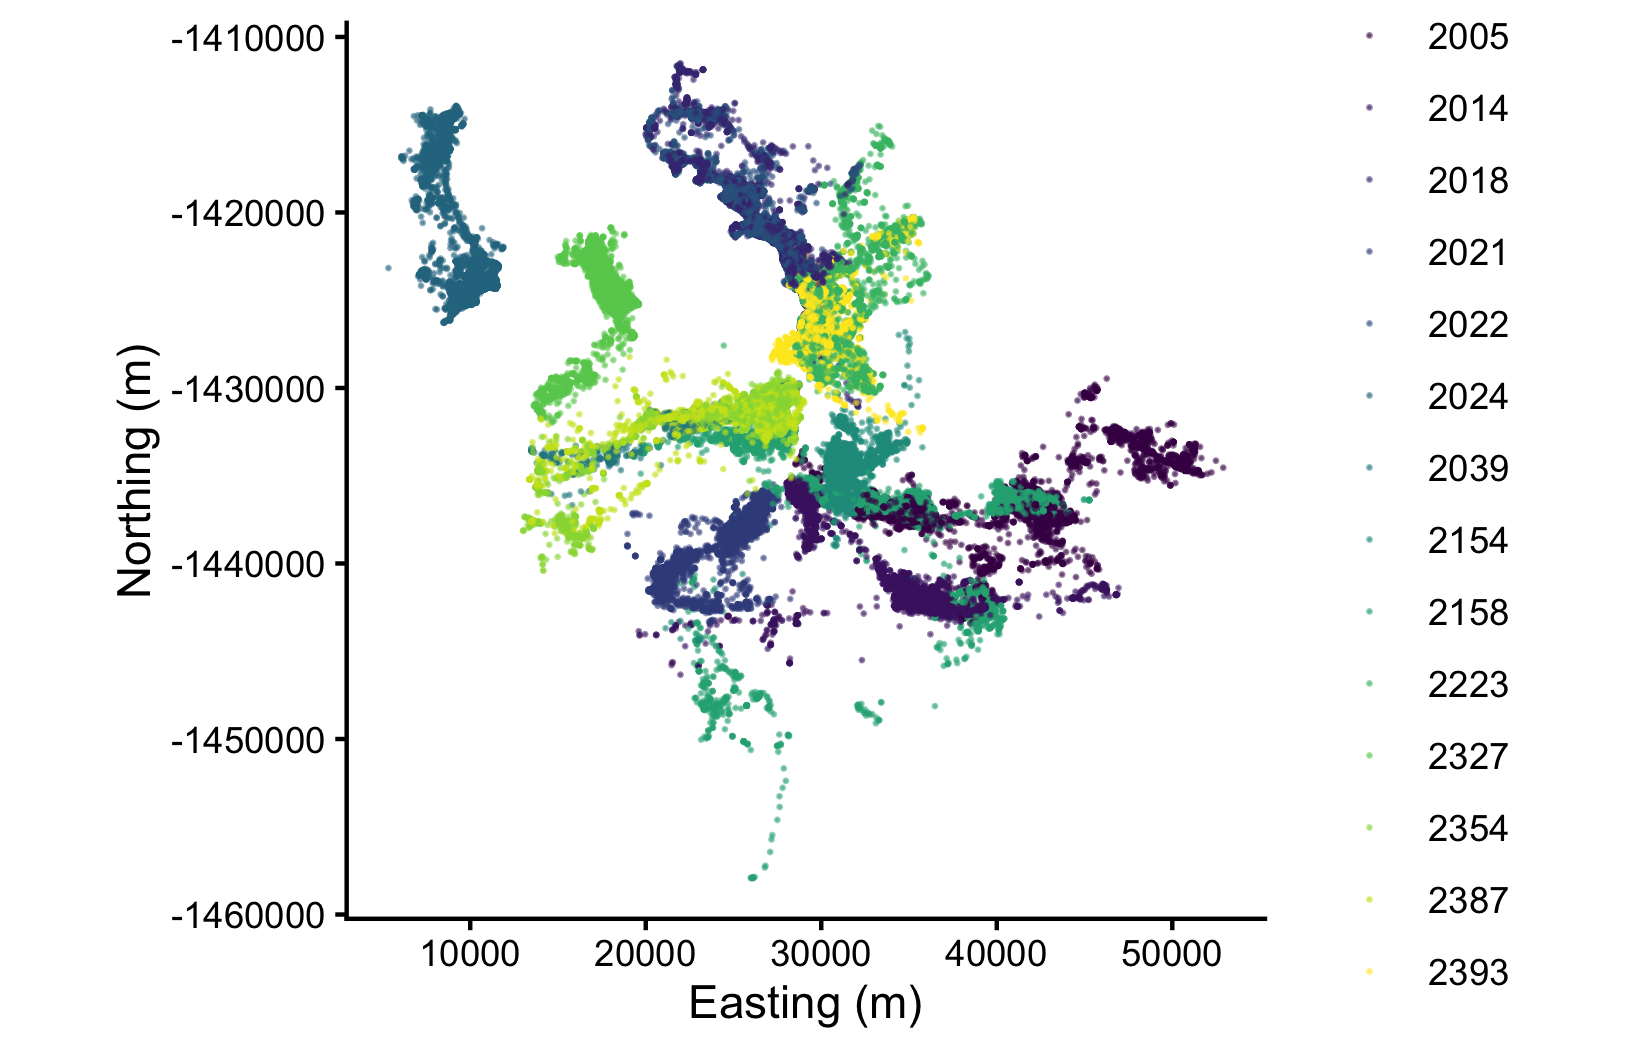
\includegraphics[keepaspectratio]{predictive_SSF_walkthrough_files/figure-pdf/plot_all_buffalo-1.png}}

}

\caption{All 14 buffalo in the dataset.}

\end{figure}%

\subsection{Select a single individual and a single
season}\label{select-a-single-individual-and-a-single-season}

We restrict the analysis to \textbf{one individual over one season}, for
two reasons.

\emph{One individual} keeps the walkthrough focused on the simulation
pipeline rather than on the modelling questions that arise with multiple
animals (pooling, random effects, two-step estimation). It also makes
validation unambiguous: we compare predicted space use against
\emph{this animal's} observed locations.

\emph{One season} matters more than it might appear. Buffalo 2158 is not
range-stationary across the full 15 months of data --- it shifts roughly
20 km east during 2019. A long-term utilisation distribution validated
against the whole track would score badly for reasons that have nothing
to do with the quality of the model. Restricting to the 2018 dry season
keeps the animal within one contiguous area, and also matches our NDVI
layer, which represents August 2018.

\begin{Shaded}
\begin{Highlighting}[]
\NormalTok{buffalo\_id }\OtherTok{\textless{}{-}}\NormalTok{ buffalo\_all }\SpecialCharTok{\%\textgreater{}\%}
  \FunctionTok{filter}\NormalTok{(id }\SpecialCharTok{==}\NormalTok{ which\_buffalo,}
\NormalTok{         t\_ }\SpecialCharTok{\textgreater{}=}\NormalTok{ season\_start,}
\NormalTok{         t\_ }\SpecialCharTok{\textless{}}\NormalTok{  season\_end)}

\FunctionTok{cat}\NormalTok{(}\StringTok{"Number of locations:"}\NormalTok{, }\FunctionTok{nrow}\NormalTok{(buffalo\_id), }\StringTok{"}\SpecialCharTok{\textbackslash{}n}\StringTok{"}\NormalTok{)}
\end{Highlighting}
\end{Shaded}

\begin{verbatim}
Number of locations: 2235 
\end{verbatim}

\begin{Shaded}
\begin{Highlighting}[]
\FunctionTok{cat}\NormalTok{(}\StringTok{"Date range:"}\NormalTok{, }\FunctionTok{format}\NormalTok{(}\FunctionTok{min}\NormalTok{(buffalo\_id}\SpecialCharTok{$}\NormalTok{t\_)), }\StringTok{"to"}\NormalTok{, }\FunctionTok{format}\NormalTok{(}\FunctionTok{max}\NormalTok{(buffalo\_id}\SpecialCharTok{$}\NormalTok{t\_)), }\StringTok{"}\SpecialCharTok{\textbackslash{}n}\StringTok{"}\NormalTok{)}
\end{Highlighting}
\end{Shaded}

\begin{verbatim}
Date range: 2018-07-25 10:11:00 to 2018-10-31 23:09:20 
\end{verbatim}

\begin{Shaded}
\begin{Highlighting}[]
\NormalTok{buffalo\_id }\SpecialCharTok{\%\textgreater{}\%}
  \FunctionTok{ggplot}\NormalTok{(}\FunctionTok{aes}\NormalTok{(}\AttributeTok{x =}\NormalTok{ x\_, }\AttributeTok{y =}\NormalTok{ y\_, }\AttributeTok{colour =}\NormalTok{ t\_)) }\SpecialCharTok{+}
  \FunctionTok{geom\_path}\NormalTok{(}\AttributeTok{alpha =} \FloatTok{0.4}\NormalTok{, }\AttributeTok{linewidth =} \FloatTok{0.3}\NormalTok{) }\SpecialCharTok{+}
  \FunctionTok{geom\_point}\NormalTok{(}\AttributeTok{alpha =} \FloatTok{0.5}\NormalTok{, }\AttributeTok{size =} \FloatTok{0.3}\NormalTok{) }\SpecialCharTok{+}
  \FunctionTok{coord\_fixed}\NormalTok{() }\SpecialCharTok{+}
  \FunctionTok{scale\_x\_continuous}\NormalTok{(}\StringTok{"Easting (m)"}\NormalTok{) }\SpecialCharTok{+}
  \FunctionTok{scale\_y\_continuous}\NormalTok{(}\StringTok{"Northing (m)"}\NormalTok{) }\SpecialCharTok{+}
  \FunctionTok{scale\_colour\_viridis\_c}\NormalTok{(}\StringTok{"Date"}\NormalTok{, }\AttributeTok{trans =} \StringTok{"time"}\NormalTok{) }\SpecialCharTok{+}
  \FunctionTok{theme\_classic}\NormalTok{()}
\end{Highlighting}
\end{Shaded}

\begin{figure}[H]

{\centering \pandocbounded{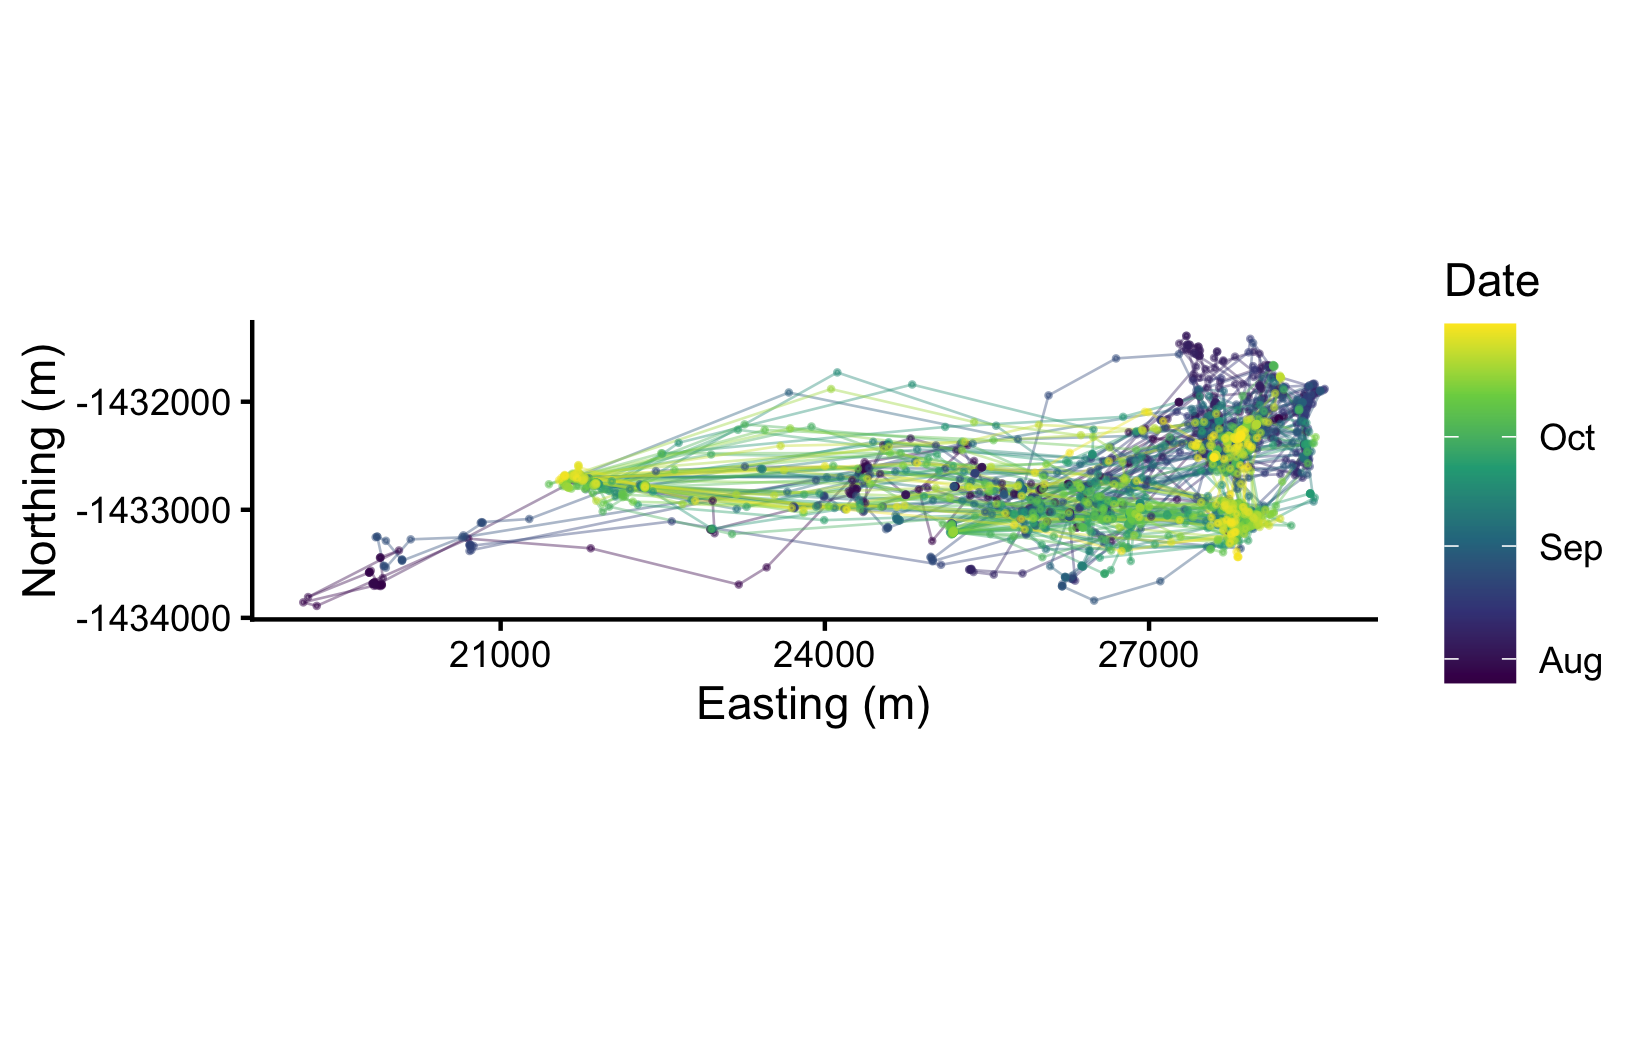
\includegraphics[keepaspectratio]{predictive_SSF_walkthrough_files/figure-pdf/plot_individual-1.png}}

}

\caption{The trajectory of the focal individual over the 2018 dry
season.}

\end{figure}%

\subsection{Check the sampling rate}\label{check-the-sampling-rate}

Step selection analysis assumes a \emph{regular} sampling interval.
Before going further we check that assumption, because irregular fixes
would make step lengths incomparable and would corrupt the mapping
between step number and hour of day that the whole temporal analysis
depends on.

\begin{Shaded}
\begin{Highlighting}[]
\FunctionTok{summarize\_sampling\_rate}\NormalTok{(buffalo\_id)}
\end{Highlighting}
\end{Shaded}

\begin{verbatim}
# A tibble: 1 x 9
    min    q1 median  mean    q3   max    sd     n unit 
  <dbl> <dbl>  <dbl> <dbl> <dbl> <dbl> <dbl> <int> <chr>
1 0.961 0.994      1  1.06  1.01  4.02 0.314  2234 hour 
\end{verbatim}

\begin{Shaded}
\begin{Highlighting}[]
\NormalTok{sampling\_intervals }\OtherTok{\textless{}{-}} \FunctionTok{as.numeric}\NormalTok{(}\FunctionTok{diff}\NormalTok{(buffalo\_id}\SpecialCharTok{$}\NormalTok{t\_), }\AttributeTok{units =} \StringTok{"hours"}\NormalTok{)}

\FunctionTok{ggplot}\NormalTok{(}\FunctionTok{data.frame}\NormalTok{(}\AttributeTok{dt =}\NormalTok{ sampling\_intervals[sampling\_intervals }\SpecialCharTok{\textless{}} \DecValTok{6}\NormalTok{]), }\FunctionTok{aes}\NormalTok{(}\AttributeTok{x =}\NormalTok{ dt)) }\SpecialCharTok{+}
  \FunctionTok{geom\_histogram}\NormalTok{(}\AttributeTok{bins =} \DecValTok{60}\NormalTok{, }\AttributeTok{fill =} \StringTok{"steelblue"}\NormalTok{, }\AttributeTok{colour =} \StringTok{"white"}\NormalTok{) }\SpecialCharTok{+}
  \FunctionTok{geom\_vline}\NormalTok{(}\AttributeTok{xintercept =} \DecValTok{1}\NormalTok{, }\AttributeTok{linetype =} \StringTok{"dashed"}\NormalTok{, }\AttributeTok{colour =} \StringTok{"red"}\NormalTok{) }\SpecialCharTok{+}
  \FunctionTok{labs}\NormalTok{(}\AttributeTok{x =} \StringTok{"Interval between fixes (hours)"}\NormalTok{, }\AttributeTok{y =} \StringTok{"Count"}\NormalTok{) }\SpecialCharTok{+}
  \FunctionTok{theme\_classic}\NormalTok{()}
\end{Highlighting}
\end{Shaded}

\begin{figure}[H]

{\centering \pandocbounded{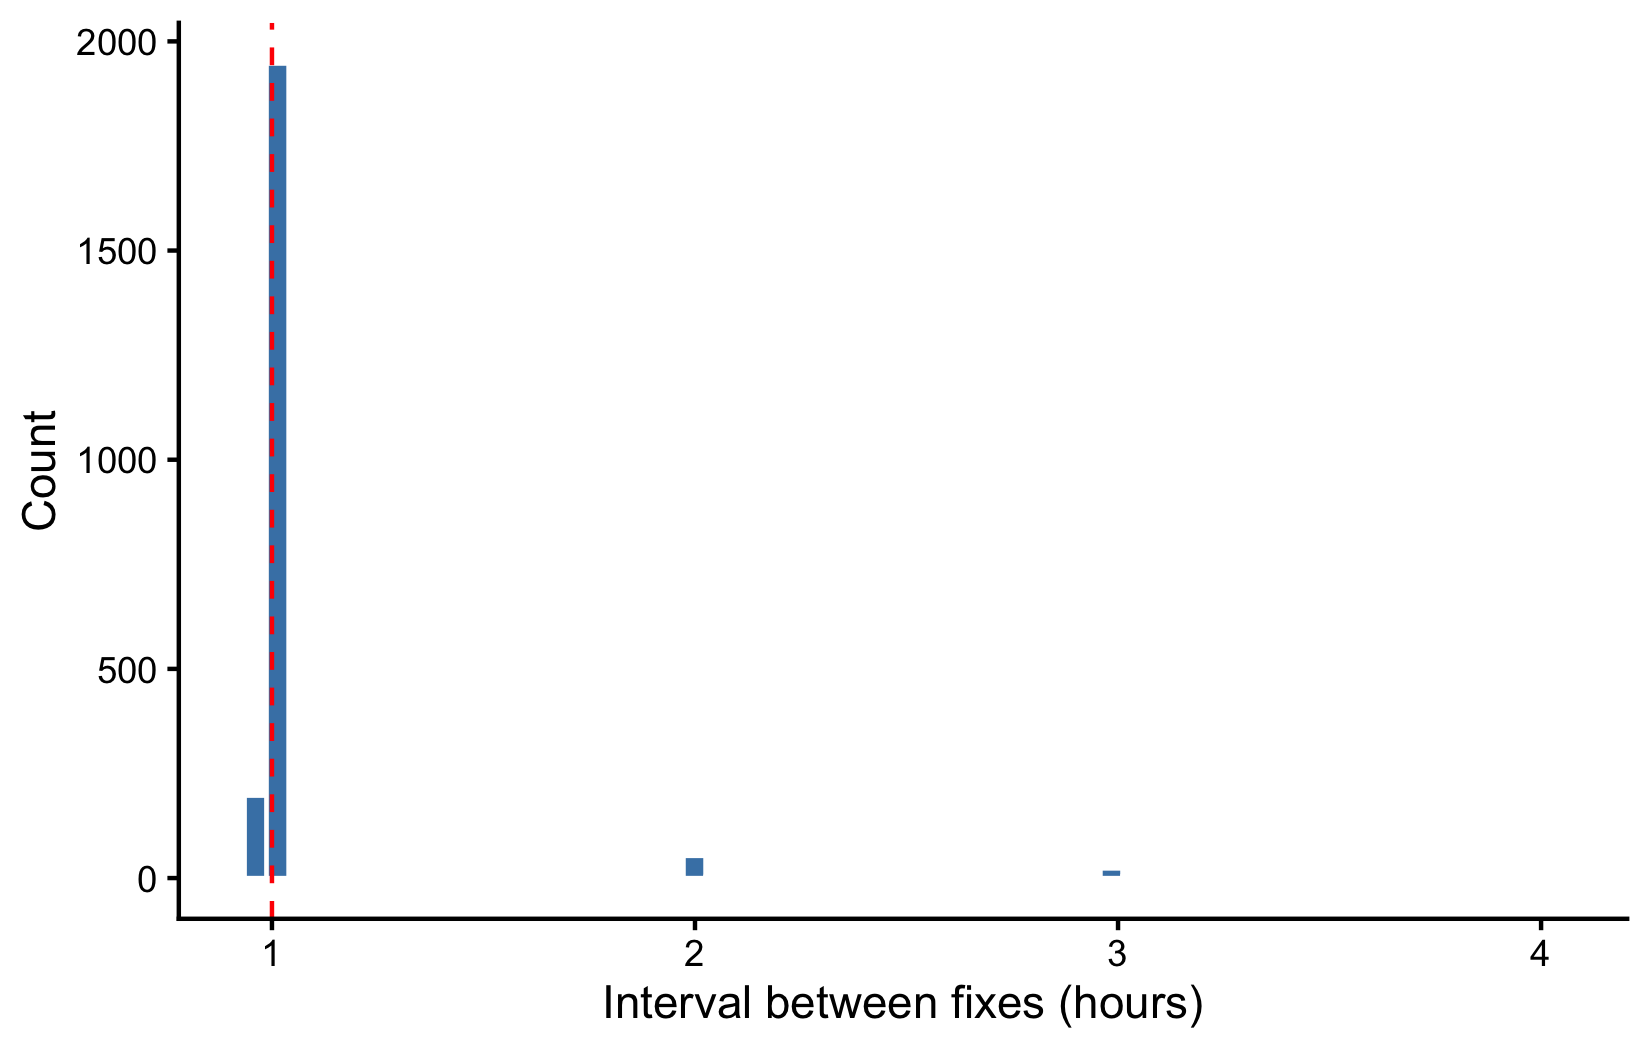
\includegraphics[keepaspectratio]{predictive_SSF_walkthrough_files/figure-pdf/plot_sampling_rate-1.png}}

}

\caption{Distribution of time intervals between consecutive fixes.}

\end{figure}%

The overwhelming majority of fixes are one hour apart, so we treat this
as an hourly trajectory.

\section{2. Environmental covariates}\label{environmental-covariates}

We use three covariates, all at 25 m resolution and on the same grid:

\begin{itemize}
\tightlist
\item
  \textbf{NDVI} --- the Normalised Difference Vegetation Index, a
  measure of vegetation greenness and productivity. Here it also
  distinguishes water bodies (strongly negative values).
\item
  \textbf{Canopy cover} --- percentage tree canopy cover, rescaled to
  0--1. Relevant for shade and thermoregulation.
\item
  \textbf{Slope} --- terrain slope in degrees.
\end{itemize}

\begin{Shaded}
\begin{Highlighting}[]
\NormalTok{ndvi }\OtherTok{\textless{}{-}} \FunctionTok{rast}\NormalTok{(}\StringTok{"mapping/ndvi\_aug\_2018.tif"}\NormalTok{)}
\FunctionTok{names}\NormalTok{(ndvi) }\OtherTok{\textless{}{-}} \StringTok{"ndvi"}

\CommentTok{\# Rescale canopy cover from a percentage (0{-}100) to a proportion (0{-}1), so that}
\CommentTok{\# its coefficient is on a scale comparable to the other covariates.}
\NormalTok{canopy }\OtherTok{\textless{}{-}} \FunctionTok{rast}\NormalTok{(}\StringTok{"mapping/canopy\_cover.tif"}\NormalTok{) }\SpecialCharTok{/} \DecValTok{100}
\FunctionTok{names}\NormalTok{(canopy) }\OtherTok{\textless{}{-}} \StringTok{"canopy"}

\NormalTok{slope }\OtherTok{\textless{}{-}} \FunctionTok{rast}\NormalTok{(}\StringTok{"mapping/slope\_raster.tif"}\NormalTok{)}
\FunctionTok{names}\NormalTok{(slope) }\OtherTok{\textless{}{-}} \StringTok{"slope"}

\CommentTok{\# All three layers share an extent and resolution, so they can be stacked directly}
\NormalTok{covariates }\OtherTok{\textless{}{-}} \FunctionTok{c}\NormalTok{(ndvi, canopy, slope)}
\NormalTok{covariates}
\end{Highlighting}
\end{Shaded}

\begin{verbatim}
class       : SpatRaster
size        : 2280, 2400, 3  (nrow, ncol, nlyr)
resolution  : 25, 25  (x, y)
extent      : 0, 60000, -1463000, -1406000  (xmin, xmax, ymin, ymax)
coord. ref. : GDA94 / Geoscience Australia Lambert (EPSG:3112)
sources     : ndvi_aug_2018.tif
              memory
              slope_raster.tif
varnames    : ndvi_aug_2018
              canopy_cover
              slope_raster
names       :      ndvi, canopy,     slope
min values  : -0.544105,      0,         0
max values  :  0.808655,  0.825, 15.833631
\end{verbatim}

\subsection{Define the simulation
extent}\label{define-the-simulation-extent}

Simulating over the full raster would be wasteful --- most of it is far
from anywhere this animal ever went, and we would need vastly more
trajectories to fill it. Instead we crop to a box around the observed
locations, with a generous buffer so that the simulated animal has
somewhere to go.

\begin{Shaded}
\begin{Highlighting}[]
\CommentTok{\# A buffered box around the observed dry{-}season locations}
\NormalTok{sim\_extent }\OtherTok{\textless{}{-}} \FunctionTok{ext}\NormalTok{(}\DecValTok{17000}\NormalTok{, }\DecValTok{31000}\NormalTok{, }\SpecialCharTok{{-}}\DecValTok{1440000}\NormalTok{, }\SpecialCharTok{{-}}\DecValTok{1426000}\NormalTok{)}

\NormalTok{covariates\_crop }\OtherTok{\textless{}{-}} \FunctionTok{crop}\NormalTok{(covariates, sim\_extent)}
\NormalTok{covariates\_crop}
\end{Highlighting}
\end{Shaded}

\begin{verbatim}
class       : SpatRaster
size        : 560, 560, 3  (nrow, ncol, nlyr)
resolution  : 25, 25  (x, y)
extent      : 17000, 31000, -1440000, -1426000  (xmin, xmax, ymin, ymax)
coord. ref. : GDA94 / Geoscience Australia Lambert (EPSG:3112)
source(s)   : memory
names       :      ndvi, canopy,    slope
min values  : -0.115635,      0, 0.000156
max values  :  0.769249,  0.825, 5.782707
\end{verbatim}

\begin{Shaded}
\begin{Highlighting}[]
\CommentTok{\# Individual layers, used throughout the rest of the script}
\NormalTok{ndvi\_crop   }\OtherTok{\textless{}{-}}\NormalTok{ covariates\_crop[[}\StringTok{"ndvi"}\NormalTok{]]}
\NormalTok{canopy\_crop }\OtherTok{\textless{}{-}}\NormalTok{ covariates\_crop[[}\StringTok{"canopy"}\NormalTok{]]}
\NormalTok{slope\_crop  }\OtherTok{\textless{}{-}}\NormalTok{ covariates\_crop[[}\StringTok{"slope"}\NormalTok{]]}
\end{Highlighting}
\end{Shaded}

\begin{Shaded}
\begin{Highlighting}[]
\FunctionTok{par}\NormalTok{(}\AttributeTok{mfrow =} \FunctionTok{c}\NormalTok{(}\DecValTok{1}\NormalTok{, }\DecValTok{3}\NormalTok{), }\AttributeTok{mar =} \FunctionTok{c}\NormalTok{(}\DecValTok{2}\NormalTok{, }\DecValTok{2}\NormalTok{, }\DecValTok{3}\NormalTok{, }\DecValTok{4}\NormalTok{))}
\ControlFlowTok{for}\NormalTok{ (lyr }\ControlFlowTok{in} \FunctionTok{c}\NormalTok{(}\StringTok{"ndvi"}\NormalTok{, }\StringTok{"canopy"}\NormalTok{, }\StringTok{"slope"}\NormalTok{)) \{}
  \FunctionTok{plot}\NormalTok{(covariates\_crop[[lyr]], }\AttributeTok{main =}\NormalTok{ lyr)}
  \FunctionTok{points}\NormalTok{(buffalo\_id}\SpecialCharTok{$}\NormalTok{x\_, buffalo\_id}\SpecialCharTok{$}\NormalTok{y\_, }\AttributeTok{col =} \FunctionTok{rgb}\NormalTok{(}\DecValTok{1}\NormalTok{, }\DecValTok{0}\NormalTok{, }\DecValTok{0}\NormalTok{, }\FloatTok{0.15}\NormalTok{), }\AttributeTok{pch =} \DecValTok{16}\NormalTok{, }\AttributeTok{cex =} \FloatTok{0.2}\NormalTok{)}
\NormalTok{\}}
\end{Highlighting}
\end{Shaded}

\begin{figure}[H]

{\centering \pandocbounded{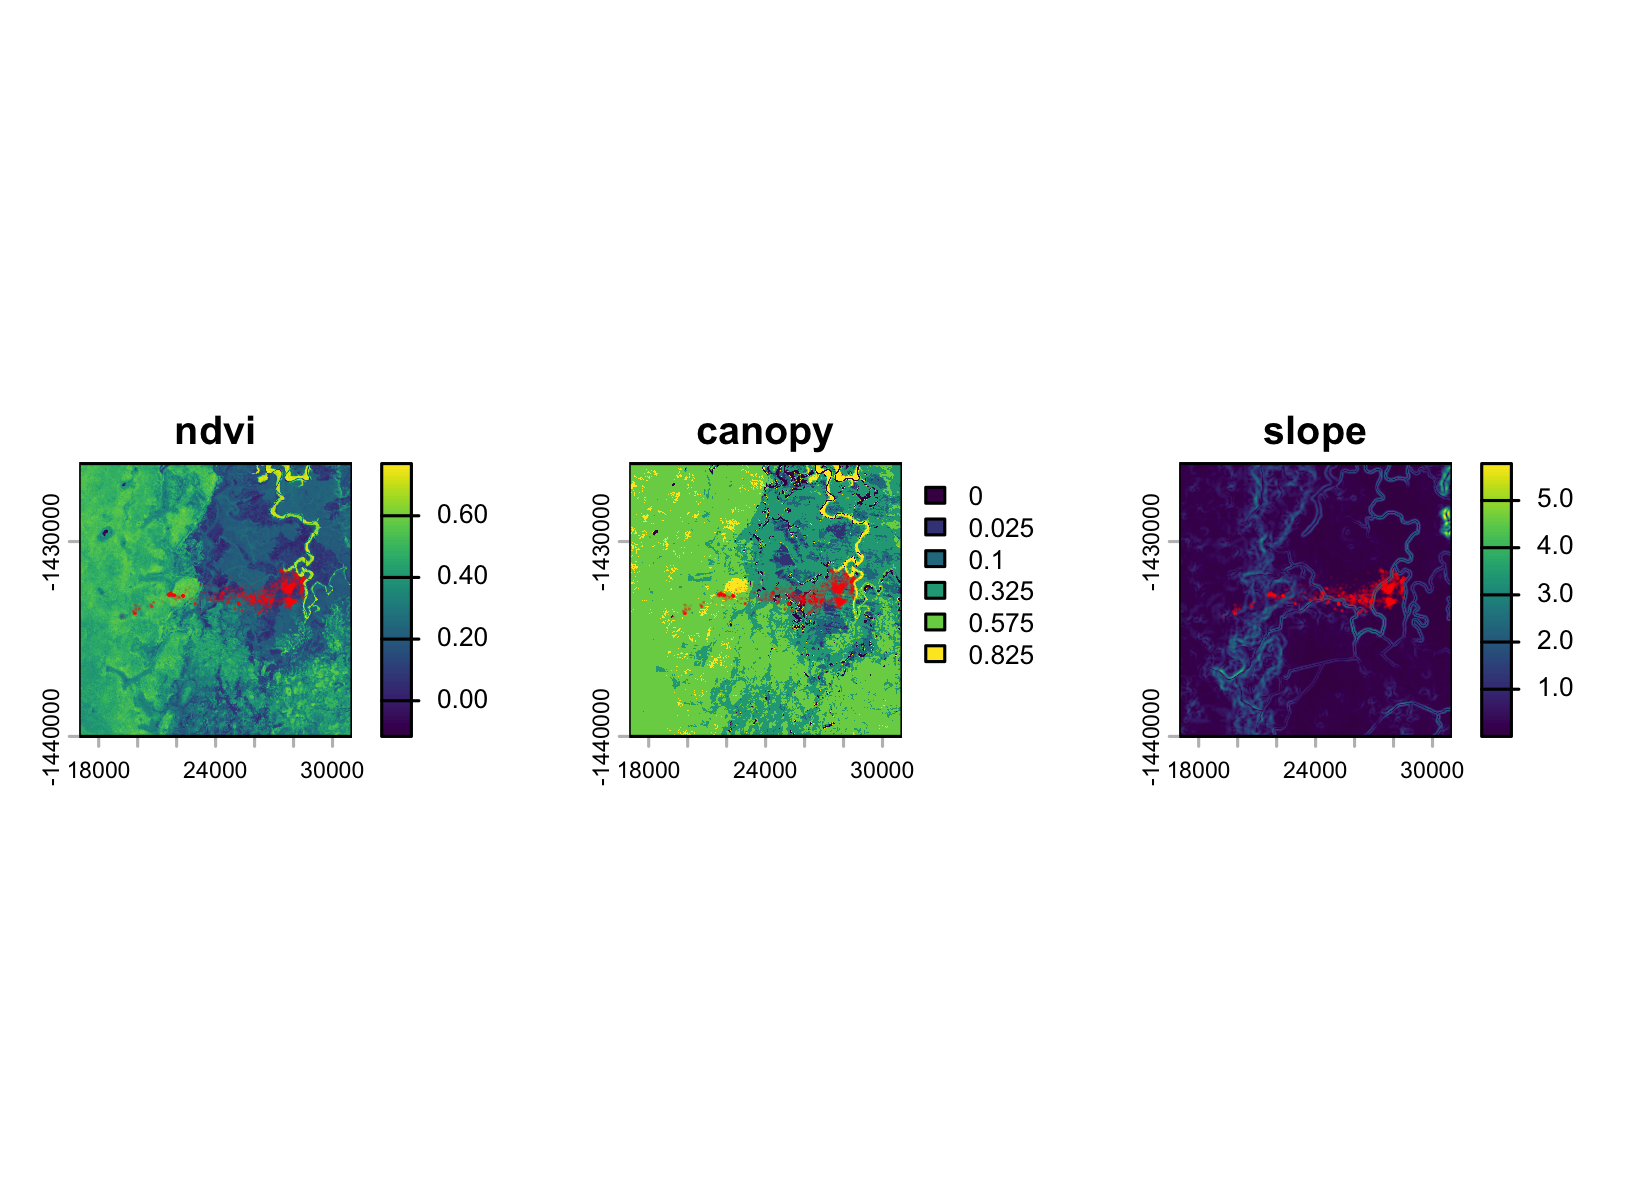
\includegraphics[keepaspectratio]{predictive_SSF_walkthrough_files/figure-pdf/plot_covariates-1.png}}

}

\caption{The three covariates across the simulation extent, with
observed locations in red.}

\end{figure}%

\begin{Shaded}
\begin{Highlighting}[]
\FunctionTok{par}\NormalTok{(}\AttributeTok{mfrow =} \FunctionTok{c}\NormalTok{(}\DecValTok{1}\NormalTok{, }\DecValTok{1}\NormalTok{))}
\end{Highlighting}
\end{Shaded}

\subsection{Used versus available: a first
look}\label{used-versus-available-a-first-look}

Before fitting anything, it is worth looking at what the animal
\emph{used} against what was \emph{available}. This is the intuition
that a habitat selection model formalises: if an animal is selecting,
the distribution of covariate values at its locations will differ from
the distribution across the landscape.

\begin{Shaded}
\begin{Highlighting}[]
\CommentTok{\# Covariate values at the observed locations}
\NormalTok{used\_vals }\OtherTok{\textless{}{-}}\NormalTok{ terra}\SpecialCharTok{::}\FunctionTok{extract}\NormalTok{(covariates\_crop,}
                            \FunctionTok{cbind}\NormalTok{(buffalo\_id}\SpecialCharTok{$}\NormalTok{x\_, buffalo\_id}\SpecialCharTok{$}\NormalTok{y\_)) }\SpecialCharTok{\%\textgreater{}\%}
  \FunctionTok{pivot\_longer}\NormalTok{(}\FunctionTok{everything}\NormalTok{(), }\AttributeTok{names\_to =} \StringTok{"covariate"}\NormalTok{, }\AttributeTok{values\_to =} \StringTok{"value"}\NormalTok{) }\SpecialCharTok{\%\textgreater{}\%}
  \FunctionTok{mutate}\NormalTok{(}\AttributeTok{source =} \StringTok{"Used"}\NormalTok{)}

\CommentTok{\# Covariate values across the whole landscape (a sample, for plotting speed)}
\NormalTok{avail\_vals }\OtherTok{\textless{}{-}}\NormalTok{ terra}\SpecialCharTok{::}\FunctionTok{spatSample}\NormalTok{(covariates\_crop, }\AttributeTok{size =} \DecValTok{20000}\NormalTok{, }\AttributeTok{na.rm =} \ConstantTok{TRUE}\NormalTok{) }\SpecialCharTok{\%\textgreater{}\%}
  \FunctionTok{pivot\_longer}\NormalTok{(}\FunctionTok{everything}\NormalTok{(), }\AttributeTok{names\_to =} \StringTok{"covariate"}\NormalTok{, }\AttributeTok{values\_to =} \StringTok{"value"}\NormalTok{) }\SpecialCharTok{\%\textgreater{}\%}
  \FunctionTok{mutate}\NormalTok{(}\AttributeTok{source =} \StringTok{"Available"}\NormalTok{)}

\FunctionTok{bind\_rows}\NormalTok{(avail\_vals, used\_vals) }\SpecialCharTok{\%\textgreater{}\%}
  \FunctionTok{filter}\NormalTok{(}\SpecialCharTok{!}\FunctionTok{is.na}\NormalTok{(value)) }\SpecialCharTok{\%\textgreater{}\%}
  \FunctionTok{ggplot}\NormalTok{(}\FunctionTok{aes}\NormalTok{(}\AttributeTok{x =}\NormalTok{ value, }\AttributeTok{fill =}\NormalTok{ source)) }\SpecialCharTok{+}
  \FunctionTok{geom\_density}\NormalTok{(}\AttributeTok{alpha =} \FloatTok{0.5}\NormalTok{, }\AttributeTok{colour =} \ConstantTok{NA}\NormalTok{) }\SpecialCharTok{+}
  \FunctionTok{facet\_wrap}\NormalTok{(}\SpecialCharTok{\textasciitilde{}}\NormalTok{ covariate, }\AttributeTok{scales =} \StringTok{"free"}\NormalTok{) }\SpecialCharTok{+}
  \FunctionTok{scale\_fill\_manual}\NormalTok{(}\AttributeTok{values =} \FunctionTok{c}\NormalTok{(}\StringTok{"Available"} \OtherTok{=} \StringTok{"grey50"}\NormalTok{, }\StringTok{"Used"} \OtherTok{=} \StringTok{"steelblue"}\NormalTok{), }\AttributeTok{name =} \ConstantTok{NULL}\NormalTok{) }\SpecialCharTok{+}
  \FunctionTok{labs}\NormalTok{(}\AttributeTok{x =} \StringTok{"Covariate value"}\NormalTok{, }\AttributeTok{y =} \StringTok{"Density"}\NormalTok{) }\SpecialCharTok{+}
  \FunctionTok{theme\_classic}\NormalTok{() }\SpecialCharTok{+}
  \FunctionTok{theme}\NormalTok{(}\AttributeTok{legend.position =} \StringTok{"bottom"}\NormalTok{)}
\end{Highlighting}
\end{Shaded}

\begin{figure}[H]

{\centering \pandocbounded{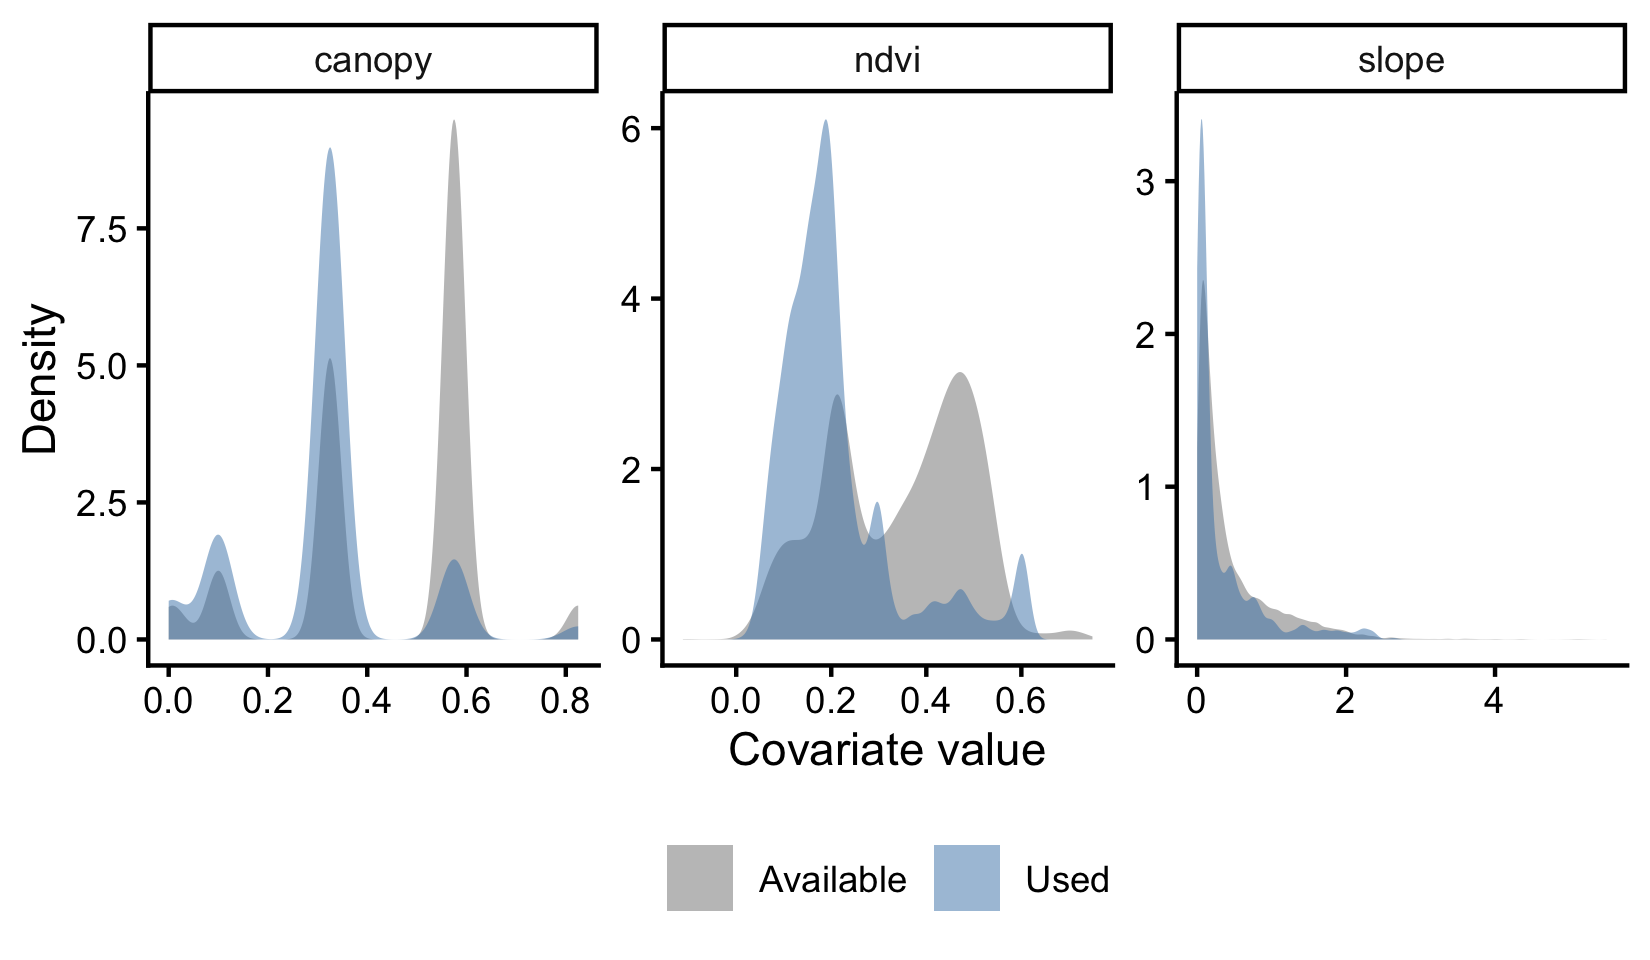
\includegraphics[keepaspectratio]{predictive_SSF_walkthrough_files/figure-pdf/used_vs_available-1.png}}

}

\caption{Distribution of covariate values across the landscape (grey)
and at observed locations (blue).}

\end{figure}%

\section{3. Generating steps and random
steps}\label{generating-steps-and-random-steps}

\subsection{From locations to steps}\label{from-locations-to-steps}

A step selection function models \emph{steps} --- the movement from one
location to the next --- rather than locations. Each step has a length
and a turning angle relative to the previous step.

\begin{Shaded}
\begin{Highlighting}[]
\NormalTok{buffalo\_steps }\OtherTok{\textless{}{-}}\NormalTok{ buffalo\_id }\SpecialCharTok{\%\textgreater{}\%} \FunctionTok{steps}\NormalTok{()}

\FunctionTok{head}\NormalTok{(buffalo\_steps)}
\end{Highlighting}
\end{Shaded}

\begin{verbatim}
# A tibble: 6 x 10
     x1_    x2_       y1_       y2_    sl_ direction_p   ta_ t1_                
*  <dbl>  <dbl>     <dbl>     <dbl>  <dbl>       <dbl> <dbl> <dttm>             
1 26818. 26607. -1432572. -1433023. 498.       -2.01   NA    2018-07-25 10:11:00
2 26607. 26610. -1433023. -1433023.   3.76     -0.0922  1.92 2018-07-25 11:10:34
3 26610. 26610. -1433023. -1433024.   1.05     -2.06   -1.97 2018-07-25 12:10:32
4 26610. 26252. -1433024. -1432758. 446.        2.50   -1.72 2018-07-25 13:10:32
5 26252. 26251. -1432758. -1432762.   3.89     -1.71    2.07 2018-07-25 16:10:44
6 26251. 26247. -1432762. -1432764.   5.33     -2.75   -1.04 2018-07-25 17:10:32
# i 2 more variables: t2_ <dttm>, dt_ <drtn>
\end{verbatim}

\subsection{Tentative movement
distributions}\label{tentative-movement-distributions}

Integrated step selection analysis (iSSA) works by first fitting
\emph{tentative} distributions to the observed step lengths and turning
angles, using those to generate available steps, and then
\textbf{correcting} them using the coefficients that the model estimates
for the movement terms (Avgar et al. 2016; Fieberg et al. 2021).

The word \emph{tentative} is important. These are not the final
estimates of the movement kernel --- they are a proposal distribution.
We recover the corrected parameters in section 6.

\begin{Shaded}
\begin{Highlighting}[]
\NormalTok{gamma\_dist    }\OtherTok{\textless{}{-}} \FunctionTok{fit\_distr}\NormalTok{(buffalo\_steps}\SpecialCharTok{$}\NormalTok{sl\_, }\StringTok{"gamma"}\NormalTok{)}
\NormalTok{vonmises\_dist }\OtherTok{\textless{}{-}} \FunctionTok{fit\_distr}\NormalTok{(buffalo\_steps}\SpecialCharTok{$}\NormalTok{ta\_, }\StringTok{"vonmises"}\NormalTok{)}

\CommentTok{\# Store the tentative parameters {-} we need them later for the update step}
\NormalTok{shape\_tentative }\OtherTok{\textless{}{-}}\NormalTok{ gamma\_dist}\SpecialCharTok{$}\NormalTok{params}\SpecialCharTok{$}\NormalTok{shape}
\NormalTok{scale\_tentative }\OtherTok{\textless{}{-}}\NormalTok{ gamma\_dist}\SpecialCharTok{$}\NormalTok{params}\SpecialCharTok{$}\NormalTok{scale}
\NormalTok{kappa\_tentative }\OtherTok{\textless{}{-}}\NormalTok{ vonmises\_dist}\SpecialCharTok{$}\NormalTok{params}\SpecialCharTok{$}\NormalTok{kappa}

\FunctionTok{cat}\NormalTok{(}\StringTok{"Tentative gamma  {-} shape:"}\NormalTok{, }\FunctionTok{round}\NormalTok{(shape\_tentative, }\DecValTok{4}\NormalTok{),}
    \StringTok{" scale:"}\NormalTok{, }\FunctionTok{round}\NormalTok{(scale\_tentative, }\DecValTok{2}\NormalTok{), }\StringTok{"}\SpecialCharTok{\textbackslash{}n}\StringTok{"}\NormalTok{)}
\end{Highlighting}
\end{Shaded}

\begin{verbatim}
Tentative gamma  - shape: 0.4266  scale: 786.79 
\end{verbatim}

\begin{Shaded}
\begin{Highlighting}[]
\FunctionTok{cat}\NormalTok{(}\StringTok{"Tentative vonMises {-} kappa:"}\NormalTok{, }\FunctionTok{round}\NormalTok{(kappa\_tentative, }\DecValTok{4}\NormalTok{), }\StringTok{"}\SpecialCharTok{\textbackslash{}n}\StringTok{"}\NormalTok{)}
\end{Highlighting}
\end{Shaded}

\begin{verbatim}
Tentative vonMises - kappa: 0.3983 
\end{verbatim}

\begin{Shaded}
\begin{Highlighting}[]
\NormalTok{p\_sl }\OtherTok{\textless{}{-}} \FunctionTok{ggplot}\NormalTok{(buffalo\_steps }\SpecialCharTok{\%\textgreater{}\%} \FunctionTok{filter}\NormalTok{(sl\_ }\SpecialCharTok{\textgreater{}} \DecValTok{0}\NormalTok{), }\FunctionTok{aes}\NormalTok{(}\AttributeTok{x =}\NormalTok{ sl\_)) }\SpecialCharTok{+}
  \FunctionTok{geom\_histogram}\NormalTok{(}\FunctionTok{aes}\NormalTok{(}\AttributeTok{y =} \FunctionTok{after\_stat}\NormalTok{(density)), }\AttributeTok{bins =} \DecValTok{80}\NormalTok{,}
                 \AttributeTok{fill =} \StringTok{"grey70"}\NormalTok{, }\AttributeTok{colour =} \StringTok{"white"}\NormalTok{) }\SpecialCharTok{+}
  \FunctionTok{stat\_function}\NormalTok{(}\AttributeTok{fun =}\NormalTok{ dgamma,}
                \AttributeTok{args =} \FunctionTok{list}\NormalTok{(}\AttributeTok{shape =}\NormalTok{ shape\_tentative, }\AttributeTok{scale =}\NormalTok{ scale\_tentative),}
                \AttributeTok{colour =} \StringTok{"red"}\NormalTok{, }\AttributeTok{linewidth =} \FloatTok{0.8}\NormalTok{) }\SpecialCharTok{+}
  \FunctionTok{scale\_x\_continuous}\NormalTok{(}\StringTok{"Step length (m)"}\NormalTok{, }\AttributeTok{limits =} \FunctionTok{c}\NormalTok{(}\DecValTok{0}\NormalTok{, }\DecValTok{2000}\NormalTok{)) }\SpecialCharTok{+}
  \FunctionTok{labs}\NormalTok{(}\AttributeTok{y =} \StringTok{"Density"}\NormalTok{) }\SpecialCharTok{+}
  \FunctionTok{theme\_classic}\NormalTok{()}

\NormalTok{p\_ta }\OtherTok{\textless{}{-}} \FunctionTok{ggplot}\NormalTok{(buffalo\_steps }\SpecialCharTok{\%\textgreater{}\%} \FunctionTok{filter}\NormalTok{(}\SpecialCharTok{!}\FunctionTok{is.na}\NormalTok{(ta\_)), }\FunctionTok{aes}\NormalTok{(}\AttributeTok{x =}\NormalTok{ ta\_)) }\SpecialCharTok{+}
  \FunctionTok{geom\_histogram}\NormalTok{(}\FunctionTok{aes}\NormalTok{(}\AttributeTok{y =} \FunctionTok{after\_stat}\NormalTok{(density)), }\AttributeTok{bins =} \DecValTok{60}\NormalTok{,}
                 \AttributeTok{fill =} \StringTok{"grey70"}\NormalTok{, }\AttributeTok{colour =} \StringTok{"white"}\NormalTok{) }\SpecialCharTok{+}
  \FunctionTok{stat\_function}\NormalTok{(}\AttributeTok{fun =} \ControlFlowTok{function}\NormalTok{(x) \{}
\NormalTok{    circular}\SpecialCharTok{::}\FunctionTok{dvonmises}\NormalTok{(circular}\SpecialCharTok{::}\FunctionTok{circular}\NormalTok{(x),}
                        \AttributeTok{mu =}\NormalTok{ circular}\SpecialCharTok{::}\FunctionTok{circular}\NormalTok{(}\DecValTok{0}\NormalTok{), }\AttributeTok{kappa =}\NormalTok{ kappa\_tentative)}
\NormalTok{  \}, }\AttributeTok{colour =} \StringTok{"red"}\NormalTok{, }\AttributeTok{linewidth =} \FloatTok{0.8}\NormalTok{) }\SpecialCharTok{+}
  \FunctionTok{scale\_x\_continuous}\NormalTok{(}\StringTok{"Turning angle (rad)"}\NormalTok{,}
                     \AttributeTok{breaks =} \FunctionTok{c}\NormalTok{(}\SpecialCharTok{{-}}\NormalTok{pi, }\SpecialCharTok{{-}}\NormalTok{pi}\SpecialCharTok{/}\DecValTok{2}\NormalTok{, }\DecValTok{0}\NormalTok{, pi}\SpecialCharTok{/}\DecValTok{2}\NormalTok{, pi),}
                     \AttributeTok{labels =} \FunctionTok{c}\NormalTok{(}\StringTok{"{-}π"}\NormalTok{, }\StringTok{"{-}π/2"}\NormalTok{, }\StringTok{"0"}\NormalTok{, }\StringTok{"π/2"}\NormalTok{, }\StringTok{"π"}\NormalTok{)) }\SpecialCharTok{+}
  \FunctionTok{labs}\NormalTok{(}\AttributeTok{y =} \StringTok{"Density"}\NormalTok{) }\SpecialCharTok{+}
  \FunctionTok{theme\_classic}\NormalTok{()}

\NormalTok{p\_sl }\SpecialCharTok{+}\NormalTok{ p\_ta}
\end{Highlighting}
\end{Shaded}

\begin{figure}[H]

{\centering \pandocbounded{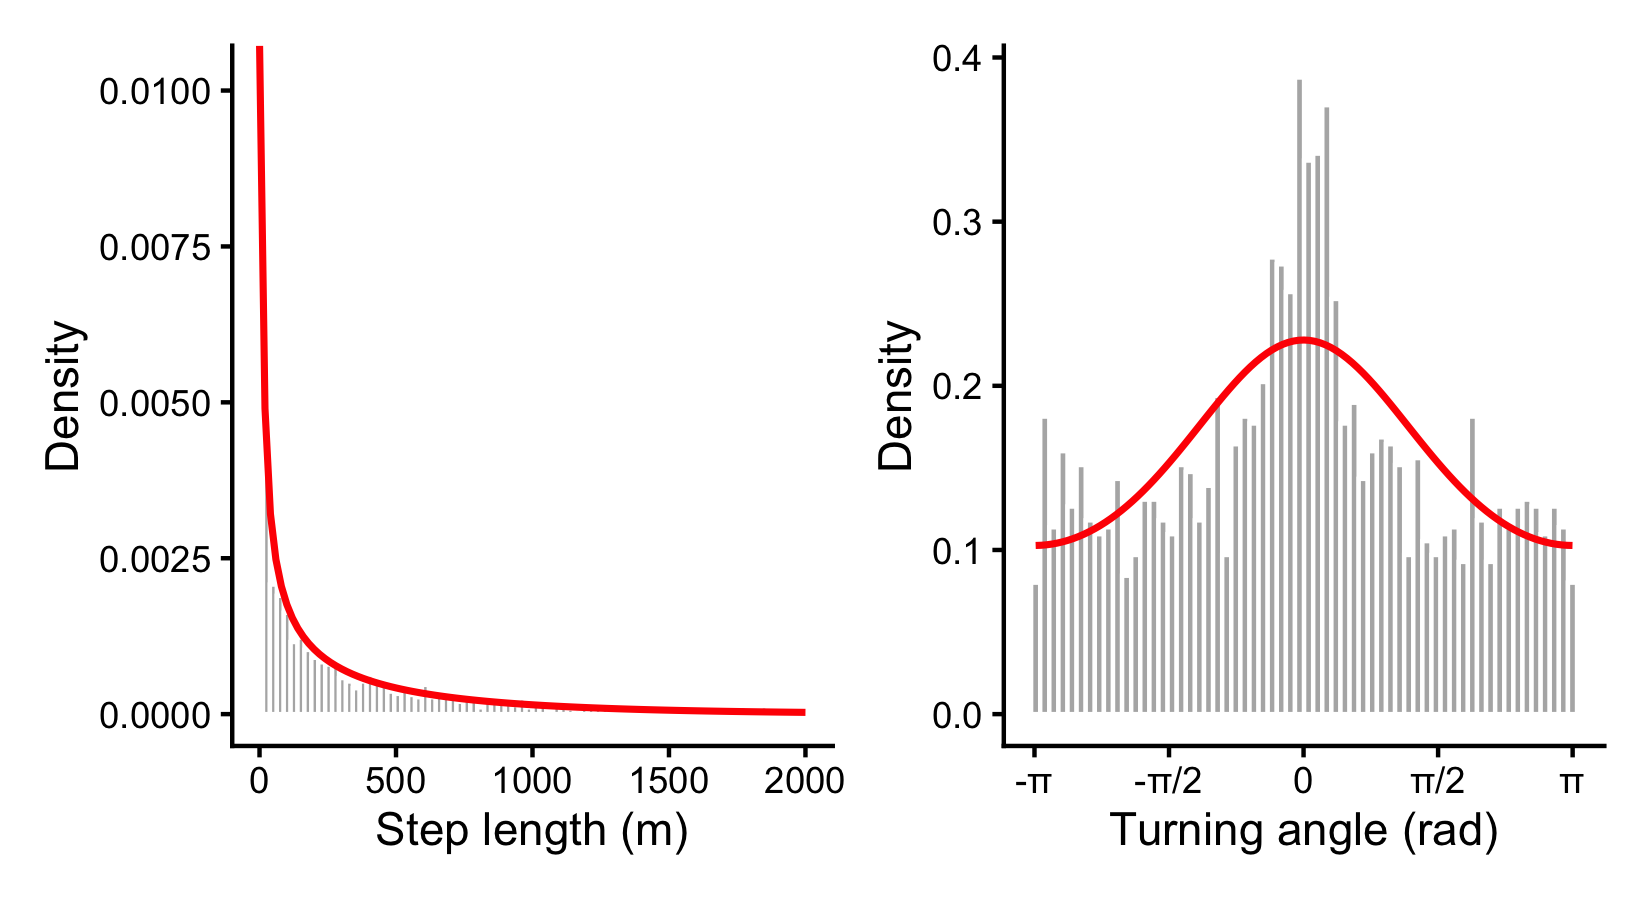
\includegraphics[keepaspectratio]{predictive_SSF_walkthrough_files/figure-pdf/plot_tentative-1.png}}

}

\caption{Observed step lengths and turning angles with the fitted
tentative distributions.}

\end{figure}%

\subsection{Sample available steps}\label{sample-available-steps}

For each observed (\emph{used}) step we generate 25 \emph{available}
steps from the tentative distributions, and extract the covariate values
at the end of every step.

Note the naming of the movement terms: \texttt{sl\_}, \texttt{log\_sl\_}
and \texttt{cos\_ta\_}, each with a \textbf{trailing underscore}. This
is \texttt{amt}'s convention, and following it means that
\texttt{amt::update\_sl\_distr()} and \texttt{amt::update\_ta\_distr()}
will work on our fitted model without any manual specification --- which
we make use of as a cross-check in section 6.

\begin{Shaded}
\begin{Highlighting}[]
\NormalTok{ssf\_data }\OtherTok{\textless{}{-}}\NormalTok{ buffalo\_steps }\SpecialCharTok{\%\textgreater{}\%}
  \FunctionTok{random\_steps}\NormalTok{(}\AttributeTok{n\_control =}\NormalTok{ n\_control,}
               \AttributeTok{sl\_distr  =}\NormalTok{ gamma\_dist,}
               \AttributeTok{ta\_distr  =}\NormalTok{ vonmises\_dist) }\SpecialCharTok{\%\textgreater{}\%}
  \FunctionTok{extract\_covariates}\NormalTok{(covariates) }\SpecialCharTok{\%\textgreater{}\%}
  \FunctionTok{mutate}\NormalTok{(}
    \AttributeTok{log\_sl\_ =} \FunctionTok{log}\NormalTok{(sl\_),}
    \AttributeTok{cos\_ta\_ =} \FunctionTok{cos}\NormalTok{(ta\_),}
    \AttributeTok{hour    =} \FunctionTok{hour}\NormalTok{(t1\_),   }\CommentTok{\# hour of day at the START of the step}
    \AttributeTok{times   =} \DecValTok{1}            \CommentTok{\# a dummy column of constant values, required by the}
                           \CommentTok{\# Cox proportional hazards family in \textasciigrave{}mgcv\textasciigrave{} (see below)}
\NormalTok{  ) }\SpecialCharTok{\%\textgreater{}\%}
  \CommentTok{\# Drop steps falling outside the covariate layers, and any zero{-}length steps}
  \CommentTok{\# (log(0) is undefined)}
  \FunctionTok{filter}\NormalTok{(}\SpecialCharTok{!}\FunctionTok{is.na}\NormalTok{(ndvi), }\SpecialCharTok{!}\FunctionTok{is.na}\NormalTok{(canopy), }\SpecialCharTok{!}\FunctionTok{is.na}\NormalTok{(slope), sl\_ }\SpecialCharTok{\textgreater{}} \DecValTok{0}\NormalTok{)}

\FunctionTok{cat}\NormalTok{(}\StringTok{"Rows:"}\NormalTok{, }\FunctionTok{nrow}\NormalTok{(ssf\_data),}
    \StringTok{" | strata (used steps):"}\NormalTok{, }\FunctionTok{length}\NormalTok{(}\FunctionTok{unique}\NormalTok{(ssf\_data}\SpecialCharTok{$}\NormalTok{step\_id\_)), }\StringTok{"}\SpecialCharTok{\textbackslash{}n}\StringTok{"}\NormalTok{)}
\end{Highlighting}
\end{Shaded}

\begin{verbatim}
Rows: 58058  | strata (used steps): 2233 
\end{verbatim}

\begin{Shaded}
\begin{Highlighting}[]
\FunctionTok{head}\NormalTok{(ssf\_data)}
\end{Highlighting}
\end{Shaded}

\begin{verbatim}
# A tibble: 6 x 18
     x1_    x2_       y1_       y2_     sl_    ta_ t1_                
*  <dbl>  <dbl>     <dbl>     <dbl>   <dbl>  <dbl> <dttm>             
1 26607. 26610. -1433023. -1433023.    3.76  1.92  2018-07-25 11:10:34
2 26607. 26729. -1433023. -1433058.  128.    1.73  2018-07-25 11:10:34
3 26607. 25301. -1433023. -1433725. 1483.   -0.639 2018-07-25 11:10:34
4 26607. 26420. -1433023. -1432609.  454.   -2.28  2018-07-25 11:10:34
5 26607. 27569. -1433023. -1433187.  976.    1.84  2018-07-25 11:10:34
6 26607. 26372. -1433023. -1433080.  242.   -0.893 2018-07-25 11:10:34
# i 11 more variables: t2_ <dttm>, dt_ <drtn>, case_ <lgl>, step_id_ <dbl>,
#   ndvi <dbl>, canopy <dbl>, slope <dbl>, log_sl_ <dbl>, cos_ta_ <dbl>,
#   hour <int>, times <dbl>
\end{verbatim}

\begin{Shaded}
\begin{Highlighting}[]
\NormalTok{ssf\_data }\SpecialCharTok{\%\textgreater{}\%}
  \FunctionTok{select}\NormalTok{(case\_, ndvi, canopy, slope) }\SpecialCharTok{\%\textgreater{}\%}
  \FunctionTok{pivot\_longer}\NormalTok{(}\FunctionTok{c}\NormalTok{(ndvi, canopy, slope), }\AttributeTok{names\_to =} \StringTok{"covariate"}\NormalTok{, }\AttributeTok{values\_to =} \StringTok{"value"}\NormalTok{) }\SpecialCharTok{\%\textgreater{}\%}
  \FunctionTok{mutate}\NormalTok{(}\AttributeTok{case\_ =} \FunctionTok{ifelse}\NormalTok{(case\_, }\StringTok{"Used"}\NormalTok{, }\StringTok{"Available"}\NormalTok{)) }\SpecialCharTok{\%\textgreater{}\%}
  \FunctionTok{ggplot}\NormalTok{(}\FunctionTok{aes}\NormalTok{(}\AttributeTok{x =}\NormalTok{ value, }\AttributeTok{fill =}\NormalTok{ case\_)) }\SpecialCharTok{+}
  \FunctionTok{geom\_density}\NormalTok{(}\AttributeTok{alpha =} \FloatTok{0.5}\NormalTok{, }\AttributeTok{colour =} \ConstantTok{NA}\NormalTok{) }\SpecialCharTok{+}
  \FunctionTok{facet\_wrap}\NormalTok{(}\SpecialCharTok{\textasciitilde{}}\NormalTok{ covariate, }\AttributeTok{scales =} \StringTok{"free"}\NormalTok{) }\SpecialCharTok{+}
  \FunctionTok{scale\_fill\_manual}\NormalTok{(}\AttributeTok{values =} \FunctionTok{c}\NormalTok{(}\StringTok{"Available"} \OtherTok{=} \StringTok{"grey50"}\NormalTok{, }\StringTok{"Used"} \OtherTok{=} \StringTok{"steelblue"}\NormalTok{), }\AttributeTok{name =} \ConstantTok{NULL}\NormalTok{) }\SpecialCharTok{+}
  \FunctionTok{labs}\NormalTok{(}\AttributeTok{x =} \StringTok{"Covariate value"}\NormalTok{, }\AttributeTok{y =} \StringTok{"Density"}\NormalTok{) }\SpecialCharTok{+}
  \FunctionTok{theme\_classic}\NormalTok{() }\SpecialCharTok{+}
  \FunctionTok{theme}\NormalTok{(}\AttributeTok{legend.position =} \StringTok{"bottom"}\NormalTok{)}
\end{Highlighting}
\end{Shaded}

\begin{figure}[H]

{\centering \pandocbounded{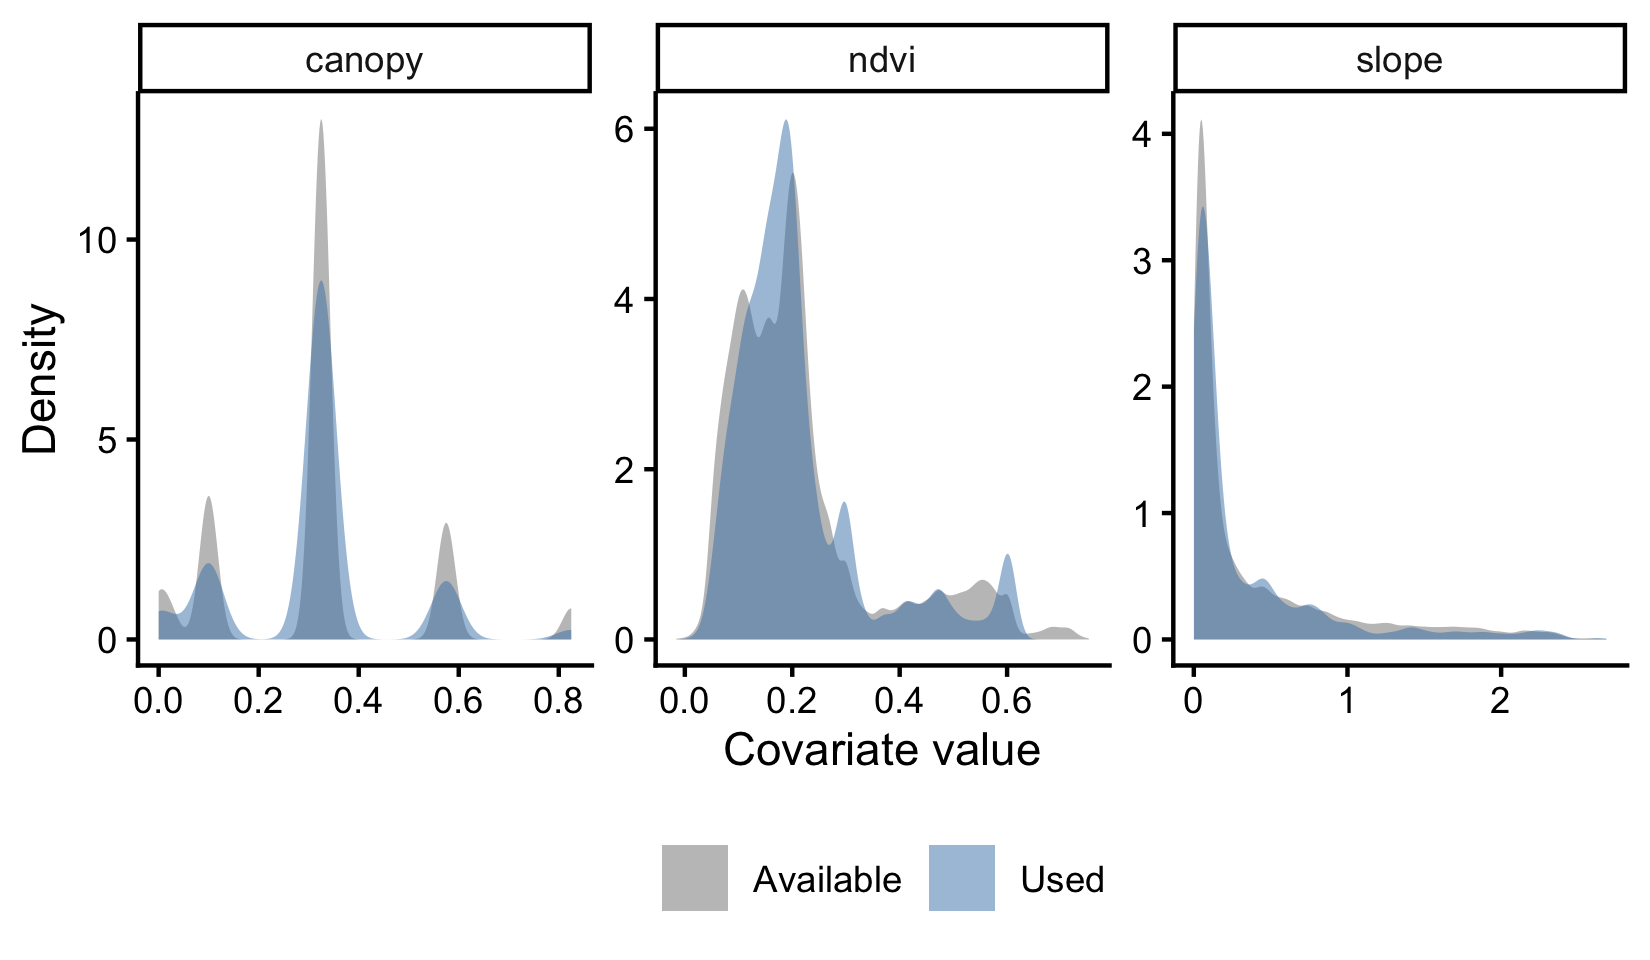
\includegraphics[keepaspectratio]{predictive_SSF_walkthrough_files/figure-pdf/plot_used_available_steps-1.png}}

}

\caption{Covariate values at the end of used steps versus available
steps.}

\end{figure}%

\section{4. Model A --- a static step selection
function}\label{model-a-a-static-step-selection-function}

\subsection{\texorpdfstring{Fitting with
\texttt{amt}}{Fitting with amt}}\label{fitting-with-amt}

The standard iSSF is fitted as a conditional logistic regression,
stratified by step.

\begin{Shaded}
\begin{Highlighting}[]
\NormalTok{ssf\_static }\OtherTok{\textless{}{-}}\NormalTok{ amt}\SpecialCharTok{::}\FunctionTok{fit\_issf}\NormalTok{(}
\NormalTok{  case\_ }\SpecialCharTok{\textasciitilde{}}\NormalTok{ ndvi }\SpecialCharTok{+}\NormalTok{ canopy }\SpecialCharTok{+}\NormalTok{ slope }\SpecialCharTok{+}      \CommentTok{\# habitat selection}
\NormalTok{    sl\_ }\SpecialCharTok{+}\NormalTok{ log\_sl\_ }\SpecialCharTok{+}\NormalTok{ cos\_ta\_ }\SpecialCharTok{+}          \CommentTok{\# movement (used to correct the tentative distributions)}
    \FunctionTok{strata}\NormalTok{(step\_id\_),                  }\CommentTok{\# each used step and its available steps form a stratum}
  \AttributeTok{data =}\NormalTok{ ssf\_data, }\AttributeTok{model =} \ConstantTok{TRUE}\NormalTok{)}

\FunctionTok{summary}\NormalTok{(ssf\_static)}
\end{Highlighting}
\end{Shaded}

\begin{verbatim}
Call:
coxph(formula = Surv(rep(1, 58058L), case_) ~ ndvi + canopy + 
    slope + sl_ + log_sl_ + cos_ta_ + strata(step_id_), data = data, 
    model = TRUE, method = "exact")

  n= 58058, number of events= 2233 

                coef    exp(coef)     se(coef)      z     Pr(>|z|)    
ndvi    -0.070265753  0.932146067  0.286238809 -0.245        0.806    
canopy  -0.156371679  0.855241256  0.175452857 -0.891        0.373    
slope   -0.300142750  0.740712477  0.052942644 -5.669 0.0000000143 ***
sl_      0.000007534  1.000007534  0.000053746  0.140        0.889    
log_sl_ -0.000947785  0.999052664  0.010774979 -0.088        0.930    
cos_ta_ -0.001306695  0.998694158  0.031398669 -0.042        0.967    
---
Signif. codes:  0 '***' 0.001 '**' 0.01 '*' 0.05 '.' 0.1 ' ' 1

        exp(coef) exp(-coef) lower .95 upper .95
ndvi       0.9321      1.073    0.5319    1.6335
canopy     0.8552      1.169    0.6064    1.2062
slope      0.7407      1.350    0.6677    0.8217
sl_        1.0000      1.000    0.9999    1.0001
log_sl_    0.9991      1.001    0.9782    1.0204
cos_ta_    0.9987      1.001    0.9391    1.0621

Concordance= 0.503  (se = 0.006 )
Likelihood ratio test= 39.31  on 6 df,   p=0.0000006
Wald test            = 36.21  on 6 df,   p=0.000003
Score (logrank) test = 36.48  on 6 df,   p=0.000002
\end{verbatim}

\subsection{The same model, fitted as a
GAM}\label{the-same-model-fitted-as-a-gam}

We also fit the identical model using \texttt{mgcv}, via a Cox
proportional hazards likelihood. A stratified Cox model with one
``event'' per stratum is mathematically equivalent to conditional
logistic regression, so this gives the same answer --- the trick is
described in Klappstein et al. (2024).

Why bother? Because Model B in the next section \emph{must} be fitted
this way (we need smooth terms), and having Model A in the same
framework means a single interface for prediction, and a like-for-like
AIC comparison.

\begin{Shaded}
\begin{Highlighting}[]
\NormalTok{ssf\_static\_gam }\OtherTok{\textless{}{-}}\NormalTok{ mgcv}\SpecialCharTok{::}\FunctionTok{gam}\NormalTok{(}
  \FunctionTok{cbind}\NormalTok{(times, step\_id\_) }\SpecialCharTok{\textasciitilde{}}\NormalTok{ ndvi }\SpecialCharTok{+}\NormalTok{ canopy }\SpecialCharTok{+}\NormalTok{ slope }\SpecialCharTok{+}\NormalTok{ sl\_ }\SpecialCharTok{+}\NormalTok{ log\_sl\_ }\SpecialCharTok{+}\NormalTok{ cos\_ta\_,}
  \AttributeTok{data =}\NormalTok{ ssf\_data, }\AttributeTok{family =}\NormalTok{ cox.ph, }\AttributeTok{weight =}\NormalTok{ case\_)}

\FunctionTok{summary}\NormalTok{(ssf\_static\_gam)}
\end{Highlighting}
\end{Shaded}

\begin{verbatim}

Family: Cox PH 
Link function: identity 

Formula:
cbind(times, step_id_) ~ ndvi + canopy + slope + sl_ + log_sl_ + 
    cos_ta_

Parametric coefficients:
            Estimate   Std. Error z value     Pr(>|z|)    
ndvi    -0.070265753  0.286238809  -0.245        0.806    
canopy  -0.156371679  0.175452857  -0.891        0.373    
slope   -0.300142749  0.052942644  -5.669 0.0000000143 ***
sl_      0.000007534  0.000053746   0.140        0.889    
log_sl_ -0.000947785  0.010774979  -0.088        0.930    
cos_ta_ -0.001306695  0.031398669  -0.042        0.967    
---
Signif. codes:  0 '***' 0.001 '**' 0.01 '*' 0.05 '.' 0.1 ' ' 1


Deviance explained = 0.117%
-REML = 7274.3  Scale est. = 1         n = 58058
\end{verbatim}

\begin{Shaded}
\begin{Highlighting}[]
\CommentTok{\# The two parameterisations should give the same coefficients}
\FunctionTok{tibble}\NormalTok{(}
  \AttributeTok{term       =} \FunctionTok{names}\NormalTok{(}\FunctionTok{coef}\NormalTok{(ssf\_static)),}
  \AttributeTok{fit\_issf   =} \FunctionTok{as.numeric}\NormalTok{(}\FunctionTok{coef}\NormalTok{(ssf\_static)),}
  \AttributeTok{cox\_ph\_gam =} \FunctionTok{as.numeric}\NormalTok{(}\FunctionTok{coef}\NormalTok{(ssf\_static\_gam)[}\FunctionTok{names}\NormalTok{(}\FunctionTok{coef}\NormalTok{(ssf\_static))])}
\NormalTok{) }\SpecialCharTok{\%\textgreater{}\%}
  \FunctionTok{mutate}\NormalTok{(}\AttributeTok{difference =}\NormalTok{ fit\_issf }\SpecialCharTok{{-}}\NormalTok{ cox\_ph\_gam)}
\end{Highlighting}
\end{Shaded}

\begin{verbatim}
# A tibble: 6 x 4
  term       fit_issf  cox_ph_gam difference
  <chr>         <dbl>       <dbl>      <dbl>
1 ndvi    -0.0703     -0.0703      -1.69e-11
2 canopy  -0.156      -0.156        2.43e-13
3 slope   -0.300      -0.300       -7.06e-11
4 sl_      0.00000753  0.00000753  -7.47e-15
5 log_sl_ -0.000948   -0.000948    -8.29e-13
6 cos_ta_ -0.00131    -0.00131      5.12e-13
\end{verbatim}

Identical to numerical precision, as expected.

\subsection{Response curves}\label{response-curves}

We express habitat selection as \textbf{relative selection strength}
(RSS): how much more likely the animal is to select a location with a
given covariate value, relative to a reference value, all else equal
(Fieberg et al. 2021). On the log scale this is just the coefficient
multiplied by the covariate value.

\begin{Shaded}
\begin{Highlighting}[]
\CommentTok{\# A sensible range of values to plot over for each covariate: the central 99\%}
\CommentTok{\# of the values that actually occur in the landscape.}
\NormalTok{cov\_ranges }\OtherTok{\textless{}{-}} \FunctionTok{map}\NormalTok{(}\FunctionTok{c}\NormalTok{(}\StringTok{"ndvi"}\NormalTok{, }\StringTok{"canopy"}\NormalTok{, }\StringTok{"slope"}\NormalTok{), }\ControlFlowTok{function}\NormalTok{(v) \{}
\NormalTok{  q }\OtherTok{\textless{}{-}} \FunctionTok{quantile}\NormalTok{(}\FunctionTok{values}\NormalTok{(covariates\_crop[[v]]), }\AttributeTok{probs =} \FunctionTok{c}\NormalTok{(}\FloatTok{0.005}\NormalTok{, }\FloatTok{0.995}\NormalTok{), }\AttributeTok{na.rm =} \ConstantTok{TRUE}\NormalTok{)}
  \FunctionTok{seq}\NormalTok{(q[}\DecValTok{1}\NormalTok{], q[}\DecValTok{2}\NormalTok{], }\AttributeTok{length.out =} \DecValTok{100}\NormalTok{)}
\NormalTok{\})}
\FunctionTok{names}\NormalTok{(cov\_ranges) }\OtherTok{\textless{}{-}} \FunctionTok{c}\NormalTok{(}\StringTok{"ndvi"}\NormalTok{, }\StringTok{"canopy"}\NormalTok{, }\StringTok{"slope"}\NormalTok{)}

\CommentTok{\# For each covariate, predict log{-}RSS across its range while holding the others}
\CommentTok{\# at zero. Because the model is linear and has no intercept, the prediction is}
\CommentTok{\# simply value * coefficient {-} but using predict() gives us standard errors,}
\CommentTok{\# and generalises to the GAM in the next section.}
\NormalTok{static\_curves }\OtherTok{\textless{}{-}} \FunctionTok{map\_dfr}\NormalTok{(}\FunctionTok{names}\NormalTok{(cov\_ranges), }\ControlFlowTok{function}\NormalTok{(v) \{}
\NormalTok{  nd }\OtherTok{\textless{}{-}} \FunctionTok{data.frame}\NormalTok{(}\AttributeTok{ndvi =} \DecValTok{0}\NormalTok{, }\AttributeTok{canopy =} \DecValTok{0}\NormalTok{, }\AttributeTok{slope =} \DecValTok{0}\NormalTok{,}
                   \AttributeTok{sl\_ =} \DecValTok{0}\NormalTok{, }\AttributeTok{log\_sl\_ =} \DecValTok{0}\NormalTok{, }\AttributeTok{cos\_ta\_ =} \DecValTok{0}\NormalTok{)}
\NormalTok{  nd }\OtherTok{\textless{}{-}}\NormalTok{ nd[}\FunctionTok{rep}\NormalTok{(}\DecValTok{1}\NormalTok{, }\FunctionTok{length}\NormalTok{(cov\_ranges[[v]])), ]}
\NormalTok{  nd[[v]] }\OtherTok{\textless{}{-}}\NormalTok{ cov\_ranges[[v]]}

\NormalTok{  p }\OtherTok{\textless{}{-}} \FunctionTok{predict}\NormalTok{(ssf\_static\_gam, }\AttributeTok{newdata =}\NormalTok{ nd, }\AttributeTok{type =} \StringTok{"link"}\NormalTok{, }\AttributeTok{se.fit =} \ConstantTok{TRUE}\NormalTok{)}

  \CommentTok{\# Centre on the mean covariate value, so the curve reads as "relative to average"}
\NormalTok{  ref }\OtherTok{\textless{}{-}} \FunctionTok{mean}\NormalTok{(}\FunctionTok{values}\NormalTok{(covariates\_crop[[v]]), }\AttributeTok{na.rm =} \ConstantTok{TRUE}\NormalTok{) }\SpecialCharTok{*} \FunctionTok{coef}\NormalTok{(ssf\_static\_gam)[[v]]}

  \FunctionTok{data.frame}\NormalTok{(}\AttributeTok{covariate =}\NormalTok{ v,}
             \AttributeTok{value     =}\NormalTok{ cov\_ranges[[v]],}
             \AttributeTok{log\_rss   =}\NormalTok{ p}\SpecialCharTok{$}\NormalTok{fit }\SpecialCharTok{{-}}\NormalTok{ ref,}
             \AttributeTok{lower     =}\NormalTok{ p}\SpecialCharTok{$}\NormalTok{fit }\SpecialCharTok{{-}}\NormalTok{ ref }\SpecialCharTok{{-}} \FloatTok{1.96} \SpecialCharTok{*}\NormalTok{ p}\SpecialCharTok{$}\NormalTok{se.fit,}
             \AttributeTok{upper     =}\NormalTok{ p}\SpecialCharTok{$}\NormalTok{fit }\SpecialCharTok{{-}}\NormalTok{ ref }\SpecialCharTok{+} \FloatTok{1.96} \SpecialCharTok{*}\NormalTok{ p}\SpecialCharTok{$}\NormalTok{se.fit)}
\NormalTok{\})}

\CommentTok{\# Observed values, for the rug}
\NormalTok{used\_long }\OtherTok{\textless{}{-}}\NormalTok{ ssf\_data }\SpecialCharTok{\%\textgreater{}\%}
  \FunctionTok{filter}\NormalTok{(case\_) }\SpecialCharTok{\%\textgreater{}\%}
  \FunctionTok{select}\NormalTok{(ndvi, canopy, slope) }\SpecialCharTok{\%\textgreater{}\%}
  \FunctionTok{pivot\_longer}\NormalTok{(}\FunctionTok{everything}\NormalTok{(), }\AttributeTok{names\_to =} \StringTok{"covariate"}\NormalTok{, }\AttributeTok{values\_to =} \StringTok{"value"}\NormalTok{)}

\FunctionTok{ggplot}\NormalTok{(static\_curves, }\FunctionTok{aes}\NormalTok{(}\AttributeTok{x =}\NormalTok{ value)) }\SpecialCharTok{+}
  \FunctionTok{geom\_hline}\NormalTok{(}\AttributeTok{yintercept =} \DecValTok{0}\NormalTok{, }\AttributeTok{linetype =} \StringTok{"dashed"}\NormalTok{, }\AttributeTok{colour =} \StringTok{"grey50"}\NormalTok{) }\SpecialCharTok{+}
  \FunctionTok{geom\_ribbon}\NormalTok{(}\FunctionTok{aes}\NormalTok{(}\AttributeTok{ymin =}\NormalTok{ lower, }\AttributeTok{ymax =}\NormalTok{ upper), }\AttributeTok{fill =} \StringTok{"grey70"}\NormalTok{, }\AttributeTok{alpha =} \FloatTok{0.5}\NormalTok{) }\SpecialCharTok{+}
  \FunctionTok{geom\_line}\NormalTok{(}\FunctionTok{aes}\NormalTok{(}\AttributeTok{y =}\NormalTok{ log\_rss), }\AttributeTok{linewidth =} \FloatTok{0.9}\NormalTok{) }\SpecialCharTok{+}
  \FunctionTok{geom\_rug}\NormalTok{(}\AttributeTok{data =}\NormalTok{ used\_long, }\FunctionTok{aes}\NormalTok{(}\AttributeTok{x =}\NormalTok{ value), }\AttributeTok{inherit.aes =} \ConstantTok{FALSE}\NormalTok{,}
           \AttributeTok{alpha =} \FloatTok{0.05}\NormalTok{, }\AttributeTok{sides =} \StringTok{"b"}\NormalTok{) }\SpecialCharTok{+}
  \FunctionTok{facet\_wrap}\NormalTok{(}\SpecialCharTok{\textasciitilde{}}\NormalTok{ covariate, }\AttributeTok{scales =} \StringTok{"free\_x"}\NormalTok{) }\SpecialCharTok{+}
  \FunctionTok{labs}\NormalTok{(}\AttributeTok{x =} \StringTok{"Covariate value"}\NormalTok{, }\AttributeTok{y =} \StringTok{"log{-}RSS"}\NormalTok{) }\SpecialCharTok{+}
  \FunctionTok{theme\_classic}\NormalTok{()}
\end{Highlighting}
\end{Shaded}

\begin{figure}[H]

{\centering \pandocbounded{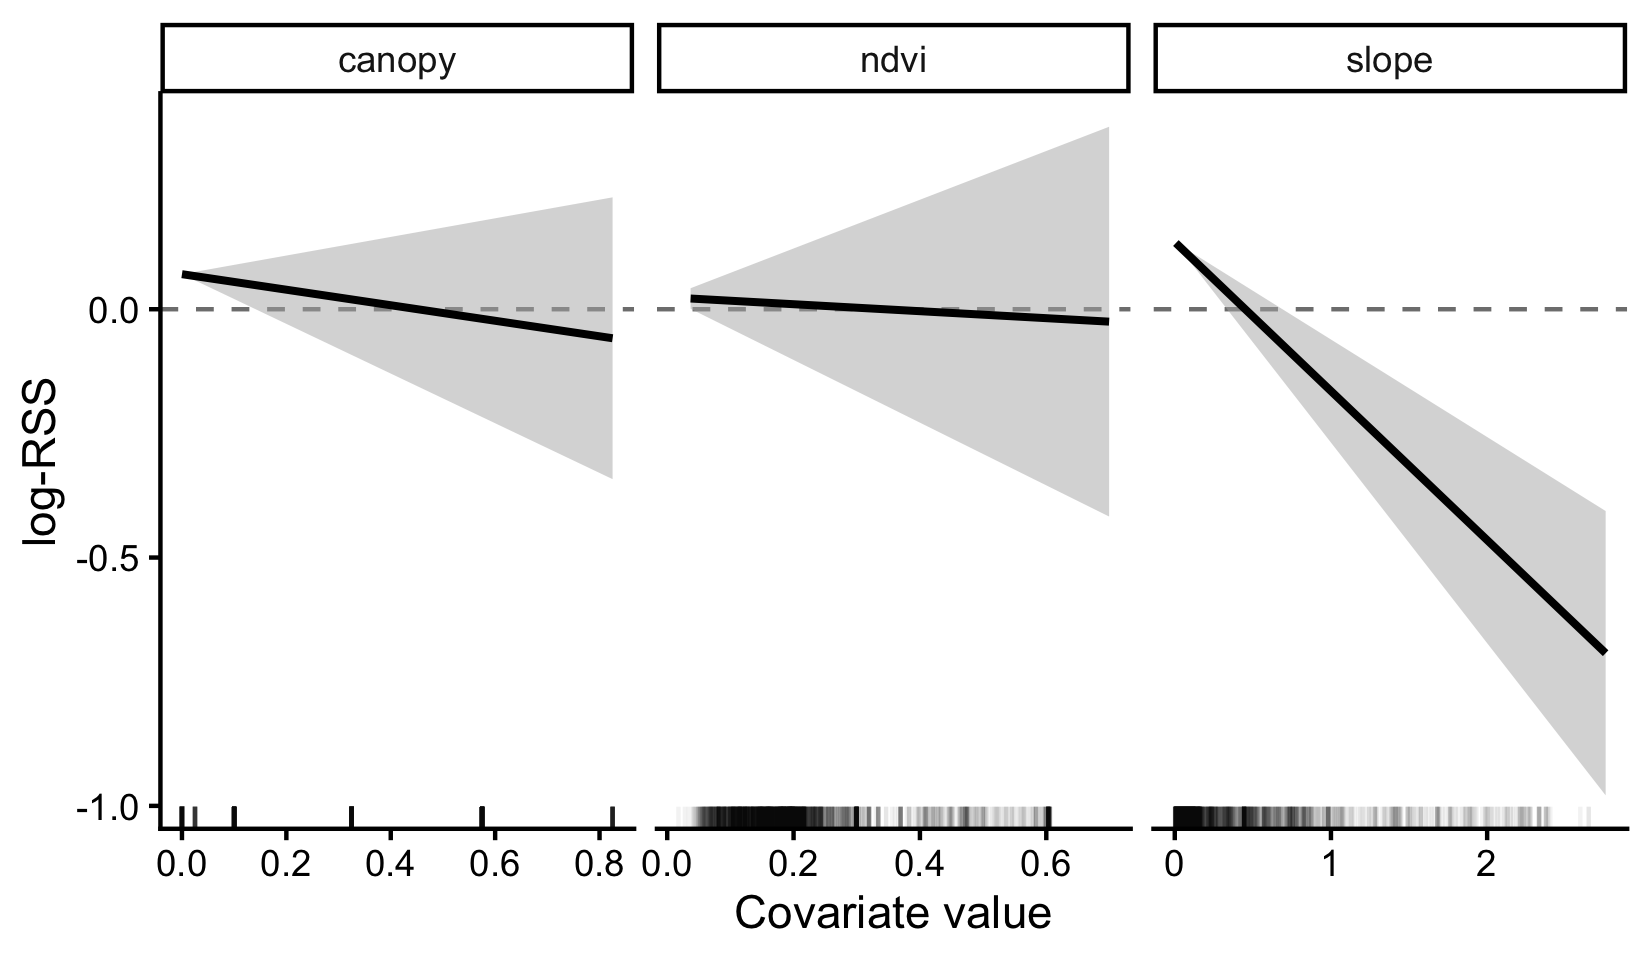
\includegraphics[keepaspectratio]{predictive_SSF_walkthrough_files/figure-pdf/static_response_curves-1.png}}

}

\caption{Log-RSS for each covariate under the static model, with 95\%
confidence intervals. Values are relative to the mean covariate value
(dashed line at zero).}

\end{figure}%

All three coefficients are negative, so on average across the whole day
this animal avoided greener, more wooded and steeper locations. Hold on
to the phrase \emph{on average across the whole day} --- it is exactly
what the next model relaxes.

\section{5. Model B --- a temporally dynamic step selection
function}\label{model-b-a-temporally-dynamic-step-selection-function}

\subsection{The idea}\label{the-idea}

Animals do not behave the same way at 3 am as at 3 pm. A buffalo may
seek shade in the heat of the day and forage in open grassland in the
evening. A static model averages over all of that, producing a
coefficient that may describe no hour of the day particularly well.

The fix is to let each coefficient be a \emph{function of time of day}:

\[
\omega(\mathbf{X}(s); \boldsymbol{\beta}(\tau)) = \exp\big(\beta_{1}(\tau) X_1(s) + \cdots + \beta_{n}(\tau) X_n(s)\big)
\]

where \(\tau\) is the hour of day. Forrest et al. (2025) expressed each
\(\beta_i(\tau)\) as a sum of harmonic (sine and cosine) terms. Here we
use a \textbf{cyclic penalised spline} instead, following Klappstein et
al. (2024) --- the idea is identical, but the smoothness is chosen
automatically by the model rather than by us picking a number of
harmonics.

In \texttt{mgcv}, \texttt{s(hour,\ by\ =\ ndvi)} fits exactly this: a
\emph{varying-coefficient} term, in which the coefficient on
\texttt{ndvi} is a smooth function of \texttt{hour}. Using
\texttt{bs\ =\ "cc"} makes that function cyclic, so it joins up smoothly
at midnight.

\subsection{Fitting the model}\label{fitting-the-model}

\begin{Shaded}
\begin{Highlighting}[]
\FunctionTok{tic}\NormalTok{(}\StringTok{"Fitting the temporally dynamic model"}\NormalTok{)}

\NormalTok{ssf\_dynamic }\OtherTok{\textless{}{-}}\NormalTok{ mgcv}\SpecialCharTok{::}\FunctionTok{gam}\NormalTok{(}
  \FunctionTok{cbind}\NormalTok{(times, step\_id\_) }\SpecialCharTok{\textasciitilde{}}
    \CommentTok{\# Habitat selection, each varying smoothly across the day}
    \FunctionTok{s}\NormalTok{(hour, }\AttributeTok{by =}\NormalTok{ ndvi,    }\AttributeTok{bs =} \StringTok{"cc"}\NormalTok{) }\SpecialCharTok{+}
    \FunctionTok{s}\NormalTok{(hour, }\AttributeTok{by =}\NormalTok{ canopy,  }\AttributeTok{bs =} \StringTok{"cc"}\NormalTok{) }\SpecialCharTok{+}
    \FunctionTok{s}\NormalTok{(hour, }\AttributeTok{by =}\NormalTok{ slope,   }\AttributeTok{bs =} \StringTok{"cc"}\NormalTok{) }\SpecialCharTok{+}
    \CommentTok{\# Movement, also varying across the day {-} this is what allows the simulated}
    \CommentTok{\# animal to travel further and more directionally at some hours than others}
    \FunctionTok{s}\NormalTok{(hour, }\AttributeTok{by =}\NormalTok{ sl\_,     }\AttributeTok{bs =} \StringTok{"cc"}\NormalTok{) }\SpecialCharTok{+}
    \FunctionTok{s}\NormalTok{(hour, }\AttributeTok{by =}\NormalTok{ log\_sl\_, }\AttributeTok{bs =} \StringTok{"cc"}\NormalTok{) }\SpecialCharTok{+}
    \FunctionTok{s}\NormalTok{(hour, }\AttributeTok{by =}\NormalTok{ cos\_ta\_, }\AttributeTok{bs =} \StringTok{"cc"}\NormalTok{),}
  \CommentTok{\# Place the cyclic knots at 0 and 24 (see the note below)}
  \AttributeTok{knots  =} \FunctionTok{list}\NormalTok{(}\AttributeTok{hour =} \FunctionTok{c}\NormalTok{(}\DecValTok{0}\NormalTok{, }\DecValTok{24}\NormalTok{)),}
  \AttributeTok{data   =}\NormalTok{ ssf\_data,}
  \AttributeTok{family =}\NormalTok{ cox.ph,}
  \AttributeTok{weight =}\NormalTok{ case\_)}

\FunctionTok{toc}\NormalTok{()}
\end{Highlighting}
\end{Shaded}

\begin{verbatim}
Fitting the temporally dynamic model: 129.425 sec elapsed
\end{verbatim}

\begin{Shaded}
\begin{Highlighting}[]
\FunctionTok{summary}\NormalTok{(ssf\_dynamic)}
\end{Highlighting}
\end{Shaded}

\begin{verbatim}

Family: Cox PH 
Link function: identity 

Formula:
cbind(times, step_id_) ~ s(hour, by = ndvi, bs = "cc") + s(hour, 
    by = canopy, bs = "cc") + s(hour, by = slope, bs = "cc") + 
    s(hour, by = sl_, bs = "cc") + s(hour, by = log_sl_, bs = "cc") + 
    s(hour, by = cos_ta_, bs = "cc")

Approximate significance of smooth terms:
                  edf Ref.df  Chi.sq             p-value    
s(hour):ndvi    7.775  8.595 113.212 <0.0000000000000002 ***
s(hour):canopy  3.038  3.772   8.325              0.0682 .  
s(hour):slope   6.979  8.016  56.125 <0.0000000000000002 ***
s(hour):sl_     8.134  8.763 219.895 <0.0000000000000002 ***
s(hour):log_sl_ 8.612  8.942 141.778 <0.0000000000000002 ***
s(hour):cos_ta_ 8.583  8.949 218.635 <0.0000000000000002 ***
---
Signif. codes:  0 '***' 0.001 '**' 0.01 '*' 0.05 '.' 0.1 ' ' 1

Deviance explained = -94.7%
-REML = 6712.6  Scale est. = 1         n = 58058
\end{verbatim}

\subsection{Two details worth knowing}\label{two-details-worth-knowing}

\subsubsection{\texorpdfstring{Why
\texttt{knots\ =\ list(hour\ =\ c(0,\ 24))}?}{Why knots = list(hour = c(0, 24))?}}\label{why-knots-listhour-c0-24}

Without this argument, \texttt{mgcv} places the endpoints of the cyclic
basis at the \emph{range of the data}. Our \texttt{hour} variable takes
integer values 0 to 23, so the endpoints would be placed at 0 and 23 ---
wrapping hour 23 onto hour 0, and squeezing an hour out of the daily
cycle. We can see this directly in the knot locations:

\begin{Shaded}
\begin{Highlighting}[]
\NormalTok{demo }\OtherTok{\textless{}{-}} \FunctionTok{data.frame}\NormalTok{(}\AttributeTok{hour =} \DecValTok{0}\SpecialCharTok{:}\DecValTok{23}\NormalTok{, }\AttributeTok{z =} \DecValTok{1}\NormalTok{)}

\CommentTok{\# Cyclic basis with the knots left to their default}
\FunctionTok{smoothCon}\NormalTok{(}\FunctionTok{s}\NormalTok{(hour, }\AttributeTok{bs =} \StringTok{"cc"}\NormalTok{, }\AttributeTok{k =} \DecValTok{6}\NormalTok{), }\AttributeTok{data =}\NormalTok{ demo, }\AttributeTok{absorb.cons =} \ConstantTok{TRUE}\NormalTok{)[[}\DecValTok{1}\NormalTok{]]}\SpecialCharTok{$}\NormalTok{xp}
\end{Highlighting}
\end{Shaded}

\begin{verbatim}
[1]  0.0  4.6  9.2 13.8 18.4 23.0
\end{verbatim}

\begin{Shaded}
\begin{Highlighting}[]
\CommentTok{\# Cyclic basis with the knots set explicitly}
\FunctionTok{smoothCon}\NormalTok{(}\FunctionTok{s}\NormalTok{(hour, }\AttributeTok{bs =} \StringTok{"cc"}\NormalTok{, }\AttributeTok{k =} \DecValTok{6}\NormalTok{), }\AttributeTok{data =}\NormalTok{ demo,}
          \AttributeTok{knots =} \FunctionTok{list}\NormalTok{(}\AttributeTok{hour =} \FunctionTok{c}\NormalTok{(}\DecValTok{0}\NormalTok{, }\DecValTok{24}\NormalTok{)), }\AttributeTok{absorb.cons =} \ConstantTok{TRUE}\NormalTok{)[[}\DecValTok{1}\NormalTok{]]}\SpecialCharTok{$}\NormalTok{xp}
\end{Highlighting}
\end{Shaded}

\begin{verbatim}
[1]  0.0  4.8  9.6 14.4 19.2 24.0
\end{verbatim}

The second is what we want: the cycle spans a full 24 hours.

\subsubsection{Do we need a parametric main effect alongside each
smooth?}\label{do-we-need-a-parametric-main-effect-alongside-each-smooth}

A reasonable worry: \texttt{mgcv} applies a sum-to-zero identifiability
constraint to smooth terms, so would \texttt{s(hour,\ by\ =\ ndvi)} be
forced to \emph{average} to zero across the day --- throwing away the
overall strength of selection, and leaving only its shape?

It would, if the \texttt{by} variable were a factor. But for a
\textbf{numeric} \texttt{by} variable \texttt{mgcv} does not apply the
centring constraint, because the smooth is already identifiable. We can
confirm this by counting the basis columns that survive the constraint:

\begin{Shaded}
\begin{Highlighting}[]
\NormalTok{demo }\OtherTok{\textless{}{-}} \FunctionTok{data.frame}\NormalTok{(}\AttributeTok{hour =} \DecValTok{0}\SpecialCharTok{:}\DecValTok{23}\NormalTok{, }\AttributeTok{z =} \FunctionTok{rnorm}\NormalTok{(}\DecValTok{24}\NormalTok{))}

\CommentTok{\# A plain smooth: one column is removed by the centring constraint (k {-} 2)}
\FunctionTok{ncol}\NormalTok{(}\FunctionTok{smoothCon}\NormalTok{(}\FunctionTok{s}\NormalTok{(hour, }\AttributeTok{bs =} \StringTok{"cc"}\NormalTok{, }\AttributeTok{k =} \DecValTok{6}\NormalTok{), }\AttributeTok{data =}\NormalTok{ demo,}
               \AttributeTok{knots =} \FunctionTok{list}\NormalTok{(}\AttributeTok{hour =} \FunctionTok{c}\NormalTok{(}\DecValTok{0}\NormalTok{, }\DecValTok{24}\NormalTok{)), }\AttributeTok{absorb.cons =} \ConstantTok{TRUE}\NormalTok{)[[}\DecValTok{1}\NormalTok{]]}\SpecialCharTok{$}\NormalTok{X)}
\end{Highlighting}
\end{Shaded}

\begin{verbatim}
[1] 4
\end{verbatim}

\begin{Shaded}
\begin{Highlighting}[]
\CommentTok{\# A smooth with a numeric \textasciigrave{}by\textasciigrave{} variable: no centring constraint applied (k {-} 1)}
\FunctionTok{ncol}\NormalTok{(}\FunctionTok{smoothCon}\NormalTok{(}\FunctionTok{s}\NormalTok{(hour, }\AttributeTok{by =}\NormalTok{ z, }\AttributeTok{bs =} \StringTok{"cc"}\NormalTok{, }\AttributeTok{k =} \DecValTok{6}\NormalTok{), }\AttributeTok{data =}\NormalTok{ demo,}
               \AttributeTok{knots =} \FunctionTok{list}\NormalTok{(}\AttributeTok{hour =} \FunctionTok{c}\NormalTok{(}\DecValTok{0}\NormalTok{, }\DecValTok{24}\NormalTok{)), }\AttributeTok{absorb.cons =} \ConstantTok{TRUE}\NormalTok{)[[}\DecValTok{1}\NormalTok{]]}\SpecialCharTok{$}\NormalTok{X)}
\end{Highlighting}
\end{Shaded}

\begin{verbatim}
[1] 5
\end{verbatim}

Five columns rather than four: the constraint is not applied. So
\texttt{s(hour,\ by\ =\ ndvi)} gives us \(\beta_{\text{NDVI}}(\tau)\)
complete, including its overall level, and there is no need to add a
parametric \texttt{ndvi} term alongside it. (Doing so would simply add a
redundant parameter.)

\subsection{Model comparison}\label{model-comparison}

\begin{Shaded}
\begin{Highlighting}[]
\FunctionTok{tibble}\NormalTok{(}
  \AttributeTok{model =} \FunctionTok{c}\NormalTok{(}\StringTok{"A: static"}\NormalTok{, }\StringTok{"B: temporally dynamic"}\NormalTok{),}
  \AttributeTok{AIC   =} \FunctionTok{c}\NormalTok{(}\FunctionTok{AIC}\NormalTok{(ssf\_static\_gam), }\FunctionTok{AIC}\NormalTok{(ssf\_dynamic)),}
  \AttributeTok{edf   =} \FunctionTok{c}\NormalTok{(}\FunctionTok{sum}\NormalTok{(ssf\_static\_gam}\SpecialCharTok{$}\NormalTok{edf), }\FunctionTok{sum}\NormalTok{(ssf\_dynamic}\SpecialCharTok{$}\NormalTok{edf))}
\NormalTok{) }\SpecialCharTok{\%\textgreater{}\%}
  \FunctionTok{mutate}\NormalTok{(}\AttributeTok{delta\_AIC =}\NormalTok{ AIC }\SpecialCharTok{{-}} \FunctionTok{min}\NormalTok{(AIC))}
\end{Highlighting}
\end{Shaded}

\begin{verbatim}
# A tibble: 2 x 4
  model                    AIC   edf delta_AIC
  <chr>                  <dbl> <dbl>     <dbl>
1 A: static             14523.   6       1212.
2 B: temporally dynamic 13311.  43.1        0 
\end{verbatim}

The dynamic model is overwhelmingly preferred. That is a statement about
\emph{fit}, though --- whether it also predicts better is the question
we take up in section 11.

\subsection{Model diagnostics}\label{model-diagnostics}

\begin{Shaded}
\begin{Highlighting}[]
\NormalTok{gratia}\SpecialCharTok{::}\FunctionTok{draw}\NormalTok{(ssf\_dynamic, }\AttributeTok{rug =} \ConstantTok{FALSE}\NormalTok{) }\SpecialCharTok{\&}
  \FunctionTok{theme\_classic}\NormalTok{()}
\end{Highlighting}
\end{Shaded}

\begin{figure}[H]

{\centering \pandocbounded{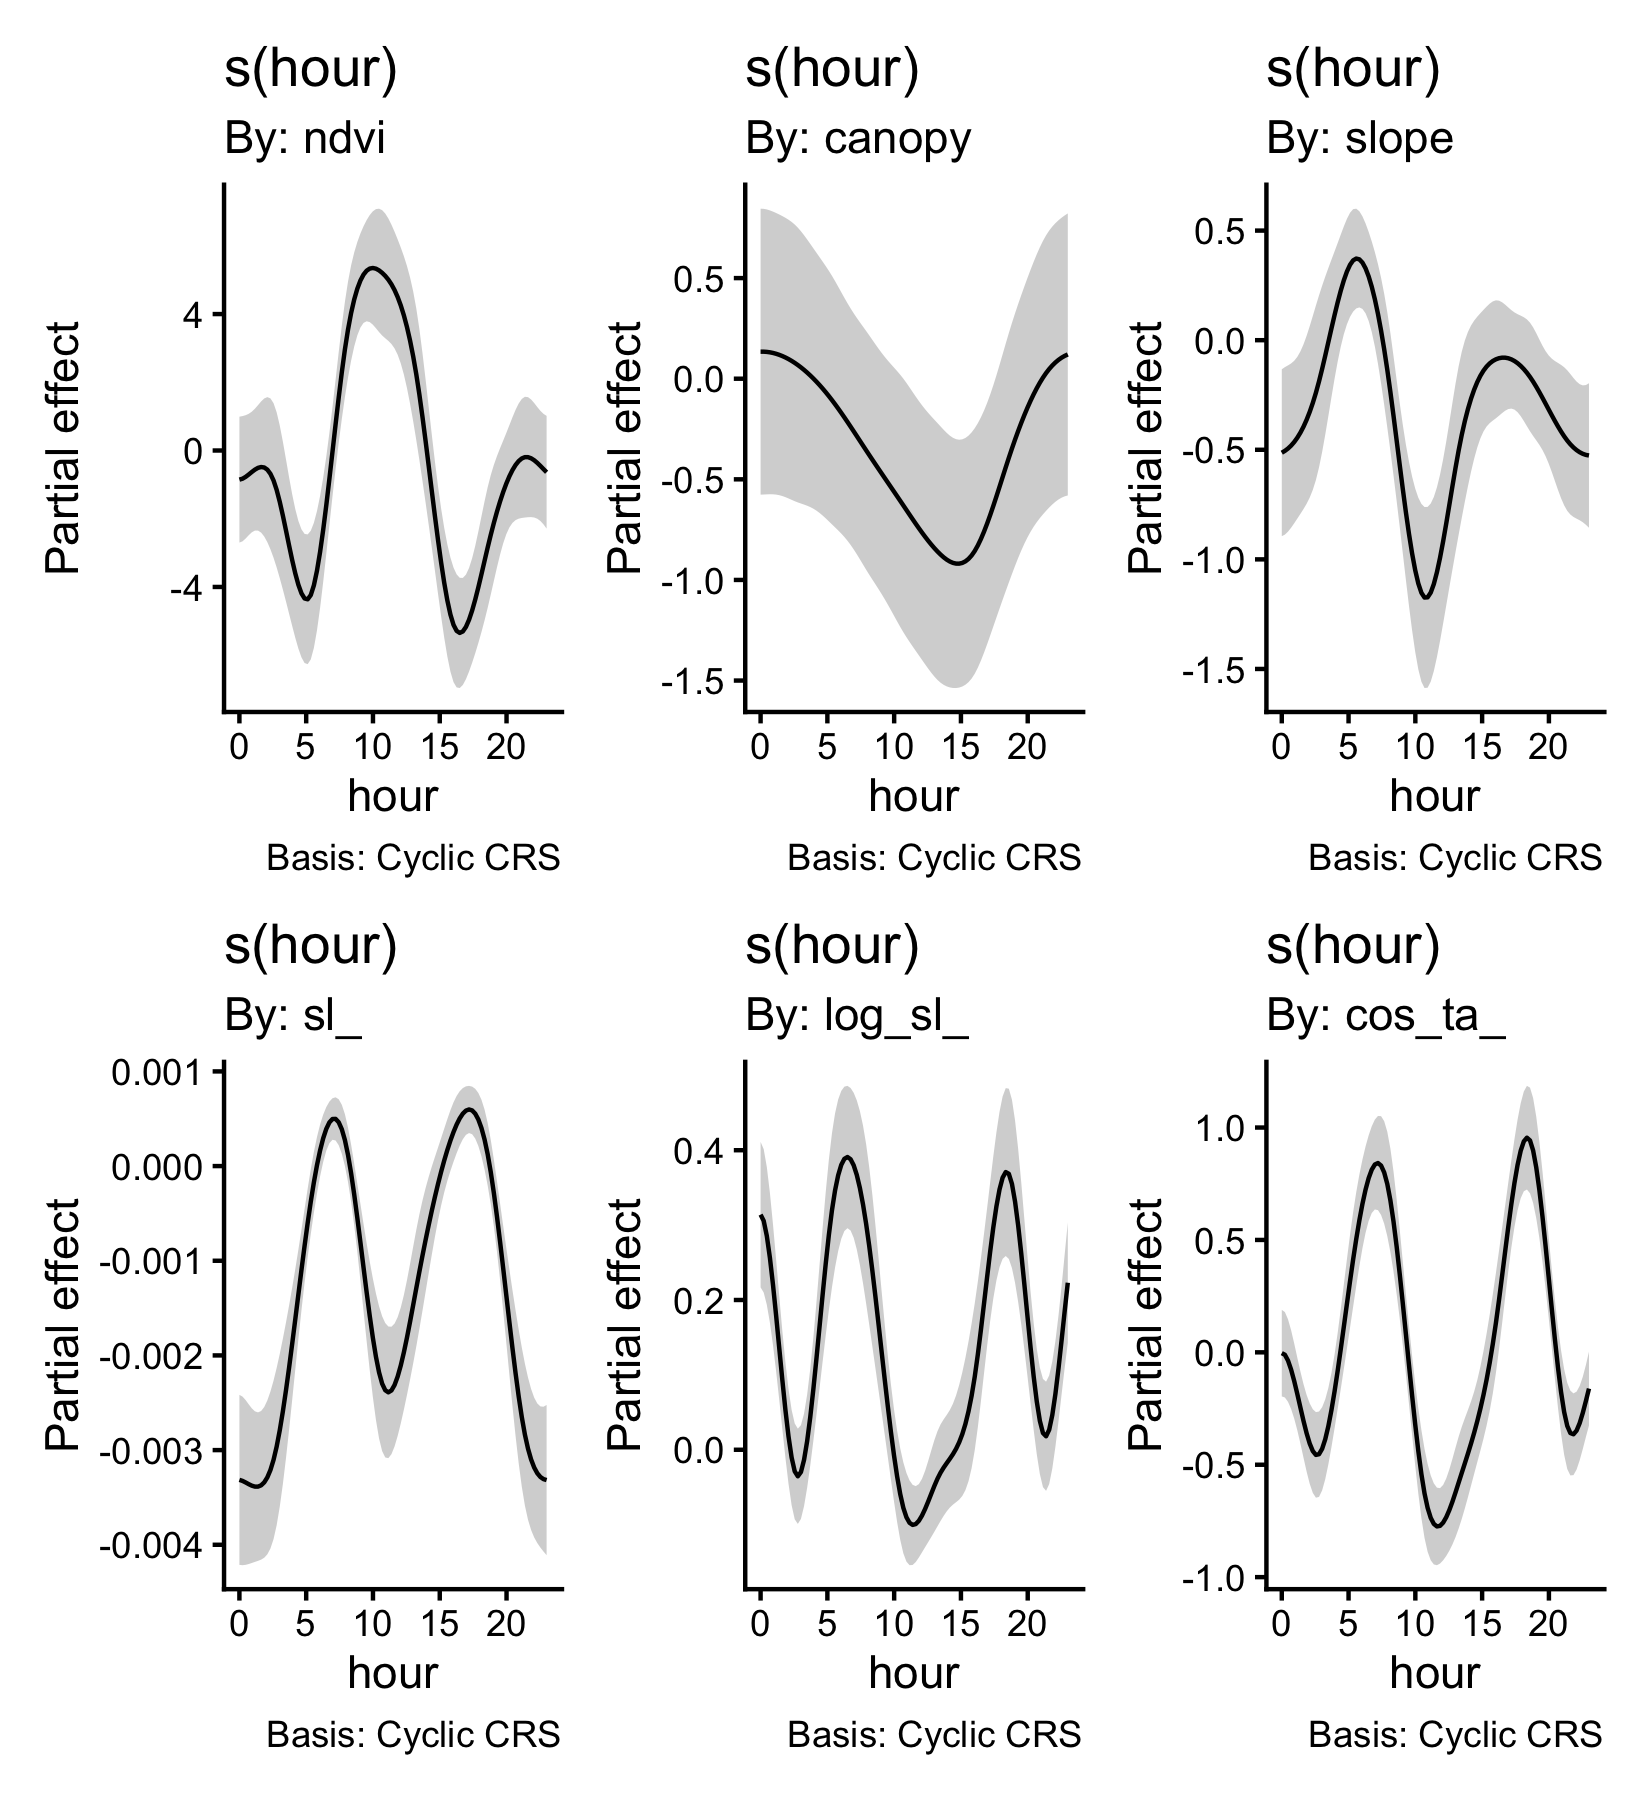
\includegraphics[keepaspectratio]{predictive_SSF_walkthrough_files/figure-pdf/gam_draw-1.png}}

}

\caption{The six estimated smooth functions. Each panel shows how the
coefficient on that term varies across the day.}

\end{figure}%

\section{6. From fitted models to hourly
coefficients}\label{from-fitted-models-to-hourly-coefficients}

This section is the bridge between model fitting and simulation, and it
is where the two models converge onto a common representation.

We reduce \textbf{each} model to the same object: a 24-row table with
one row per hour of the day, and columns for the three habitat
coefficients plus the three movement parameters. Model A's table has
identical values in every row; Model B's cycles. Everything downstream
then works for either model without modification.

\subsection{Extracting habitat
coefficients}\label{extracting-habitat-coefficients}

A neat trick makes this uniform across both models. Because neither
model has an intercept, if we predict the linear predictor at a point
where \texttt{ndvi\ =\ 1} and every other covariate is zero, the
prediction \emph{is} \(\beta_{\text{NDVI}}(\tau)\). The same call works
for the static model (giving a constant) and the dynamic one (giving the
smooth), and \texttt{se.fit\ =\ TRUE} gives us confidence intervals for
free.

\begin{Shaded}
\begin{Highlighting}[]
\CommentTok{\#\textquotesingle{} Extract the coefficient on one covariate, for each hour of the day}
\CommentTok{\#\textquotesingle{}}
\CommentTok{\#\textquotesingle{} @param model  a fitted \textasciigrave{}mgcv\textasciigrave{} model with no intercept}
\CommentTok{\#\textquotesingle{} @param var    name of the covariate whose coefficient we want}
\CommentTok{\#\textquotesingle{} @param hours  hours at which to evaluate}
\CommentTok{\#\textquotesingle{} @return a data frame of hour, estimate, standard error and 95\% CI}
\NormalTok{beta\_by\_hour }\OtherTok{\textless{}{-}} \ControlFlowTok{function}\NormalTok{(model, var, }\AttributeTok{hours =} \DecValTok{0}\SpecialCharTok{:}\DecValTok{23}\NormalTok{) \{}

  \CommentTok{\# A design where every covariate is zero except the one of interest, which is 1.}
  \CommentTok{\# The linear predictor then equals the coefficient on that covariate.}
\NormalTok{  nd }\OtherTok{\textless{}{-}} \FunctionTok{data.frame}\NormalTok{(}\AttributeTok{hour =}\NormalTok{ hours, }\AttributeTok{ndvi =} \DecValTok{0}\NormalTok{, }\AttributeTok{canopy =} \DecValTok{0}\NormalTok{, }\AttributeTok{slope =} \DecValTok{0}\NormalTok{,}
                   \AttributeTok{sl\_ =} \DecValTok{0}\NormalTok{, }\AttributeTok{log\_sl\_ =} \DecValTok{0}\NormalTok{, }\AttributeTok{cos\_ta\_ =} \DecValTok{0}\NormalTok{)}
\NormalTok{  nd[[var]] }\OtherTok{\textless{}{-}} \DecValTok{1}

\NormalTok{  p }\OtherTok{\textless{}{-}} \FunctionTok{predict}\NormalTok{(model, }\AttributeTok{newdata =}\NormalTok{ nd, }\AttributeTok{type =} \StringTok{"link"}\NormalTok{, }\AttributeTok{se.fit =} \ConstantTok{TRUE}\NormalTok{)}

  \FunctionTok{data.frame}\NormalTok{(}\AttributeTok{hour     =}\NormalTok{ hours,}
             \AttributeTok{variable =}\NormalTok{ var,}
             \AttributeTok{estimate =} \FunctionTok{as.numeric}\NormalTok{(p}\SpecialCharTok{$}\NormalTok{fit),}
             \AttributeTok{se       =} \FunctionTok{as.numeric}\NormalTok{(p}\SpecialCharTok{$}\NormalTok{se.fit)) }\SpecialCharTok{\%\textgreater{}\%}
    \FunctionTok{mutate}\NormalTok{(}\AttributeTok{lower =}\NormalTok{ estimate }\SpecialCharTok{{-}} \FloatTok{1.96} \SpecialCharTok{*}\NormalTok{ se,}
           \AttributeTok{upper =}\NormalTok{ estimate }\SpecialCharTok{+} \FloatTok{1.96} \SpecialCharTok{*}\NormalTok{ se)}
\NormalTok{\}}
\end{Highlighting}
\end{Shaded}

\begin{Shaded}
\begin{Highlighting}[]
\NormalTok{model\_terms }\OtherTok{\textless{}{-}} \FunctionTok{c}\NormalTok{(}\StringTok{"ndvi"}\NormalTok{, }\StringTok{"canopy"}\NormalTok{, }\StringTok{"slope"}\NormalTok{, }\StringTok{"sl\_"}\NormalTok{, }\StringTok{"log\_sl\_"}\NormalTok{, }\StringTok{"cos\_ta\_"}\NormalTok{)}

\NormalTok{betas\_static  }\OtherTok{\textless{}{-}} \FunctionTok{map\_dfr}\NormalTok{(model\_terms, }\SpecialCharTok{\textasciitilde{}} \FunctionTok{beta\_by\_hour}\NormalTok{(ssf\_static\_gam, .x)) }\SpecialCharTok{\%\textgreater{}\%}
  \FunctionTok{mutate}\NormalTok{(}\AttributeTok{model =} \StringTok{"A: static"}\NormalTok{)}
\NormalTok{betas\_dynamic }\OtherTok{\textless{}{-}} \FunctionTok{map\_dfr}\NormalTok{(model\_terms, }\SpecialCharTok{\textasciitilde{}} \FunctionTok{beta\_by\_hour}\NormalTok{(ssf\_dynamic, .x)) }\SpecialCharTok{\%\textgreater{}\%}
  \FunctionTok{mutate}\NormalTok{(}\AttributeTok{model =} \StringTok{"B: temporally dynamic"}\NormalTok{)}

\NormalTok{betas\_all }\OtherTok{\textless{}{-}} \FunctionTok{bind\_rows}\NormalTok{(betas\_static, betas\_dynamic)}

\FunctionTok{head}\NormalTok{(betas\_all)}
\end{Highlighting}
\end{Shaded}

\begin{verbatim}
  hour variable    estimate        se      lower     upper     model
1    0     ndvi -0.07026575 0.2862388 -0.6312938 0.4907623 A: static
2    1     ndvi -0.07026575 0.2862388 -0.6312938 0.4907623 A: static
3    2     ndvi -0.07026575 0.2862388 -0.6312938 0.4907623 A: static
4    3     ndvi -0.07026575 0.2862388 -0.6312938 0.4907623 A: static
5    4     ndvi -0.07026575 0.2862388 -0.6312938 0.4907623 A: static
6    5     ndvi -0.07026575 0.2862388 -0.6312938 0.4907623 A: static
\end{verbatim}

\begin{Shaded}
\begin{Highlighting}[]
\FunctionTok{ggplot}\NormalTok{(betas\_all, }\FunctionTok{aes}\NormalTok{(}\AttributeTok{x =}\NormalTok{ hour, }\AttributeTok{y =}\NormalTok{ estimate, }\AttributeTok{colour =}\NormalTok{ model, }\AttributeTok{fill =}\NormalTok{ model)) }\SpecialCharTok{+}
  \FunctionTok{geom\_hline}\NormalTok{(}\AttributeTok{yintercept =} \DecValTok{0}\NormalTok{, }\AttributeTok{linetype =} \StringTok{"dashed"}\NormalTok{, }\AttributeTok{colour =} \StringTok{"grey40"}\NormalTok{) }\SpecialCharTok{+}
  \FunctionTok{geom\_ribbon}\NormalTok{(}\FunctionTok{aes}\NormalTok{(}\AttributeTok{ymin =}\NormalTok{ lower, }\AttributeTok{ymax =}\NormalTok{ upper), }\AttributeTok{alpha =} \FloatTok{0.2}\NormalTok{, }\AttributeTok{colour =} \ConstantTok{NA}\NormalTok{) }\SpecialCharTok{+}
  \FunctionTok{geom\_line}\NormalTok{(}\AttributeTok{linewidth =} \FloatTok{0.8}\NormalTok{) }\SpecialCharTok{+}
  \FunctionTok{facet\_wrap}\NormalTok{(}\SpecialCharTok{\textasciitilde{}}\NormalTok{ variable, }\AttributeTok{scales =} \StringTok{"free\_y"}\NormalTok{) }\SpecialCharTok{+}
  \FunctionTok{scale\_colour\_manual}\NormalTok{(}\AttributeTok{values =} \FunctionTok{c}\NormalTok{(}\StringTok{"A: static"} \OtherTok{=} \StringTok{"grey40"}\NormalTok{,}
                                 \StringTok{"B: temporally dynamic"} \OtherTok{=} \StringTok{"steelblue"}\NormalTok{), }\AttributeTok{name =} \ConstantTok{NULL}\NormalTok{) }\SpecialCharTok{+}
  \FunctionTok{scale\_fill\_manual}\NormalTok{(}\AttributeTok{values =} \FunctionTok{c}\NormalTok{(}\StringTok{"A: static"} \OtherTok{=} \StringTok{"grey40"}\NormalTok{,}
                               \StringTok{"B: temporally dynamic"} \OtherTok{=} \StringTok{"steelblue"}\NormalTok{), }\AttributeTok{name =} \ConstantTok{NULL}\NormalTok{) }\SpecialCharTok{+}
  \FunctionTok{scale\_x\_continuous}\NormalTok{(}\StringTok{"Hour of day"}\NormalTok{, }\AttributeTok{breaks =} \FunctionTok{seq}\NormalTok{(}\DecValTok{0}\NormalTok{, }\DecValTok{24}\NormalTok{, }\DecValTok{6}\NormalTok{)) }\SpecialCharTok{+}
  \FunctionTok{labs}\NormalTok{(}\AttributeTok{y =} \StringTok{"Coefficient"}\NormalTok{) }\SpecialCharTok{+}
  \FunctionTok{theme\_classic}\NormalTok{() }\SpecialCharTok{+}
  \FunctionTok{theme}\NormalTok{(}\AttributeTok{legend.position =} \StringTok{"bottom"}\NormalTok{)}
\end{Highlighting}
\end{Shaded}

\begin{figure}[H]

{\centering \pandocbounded{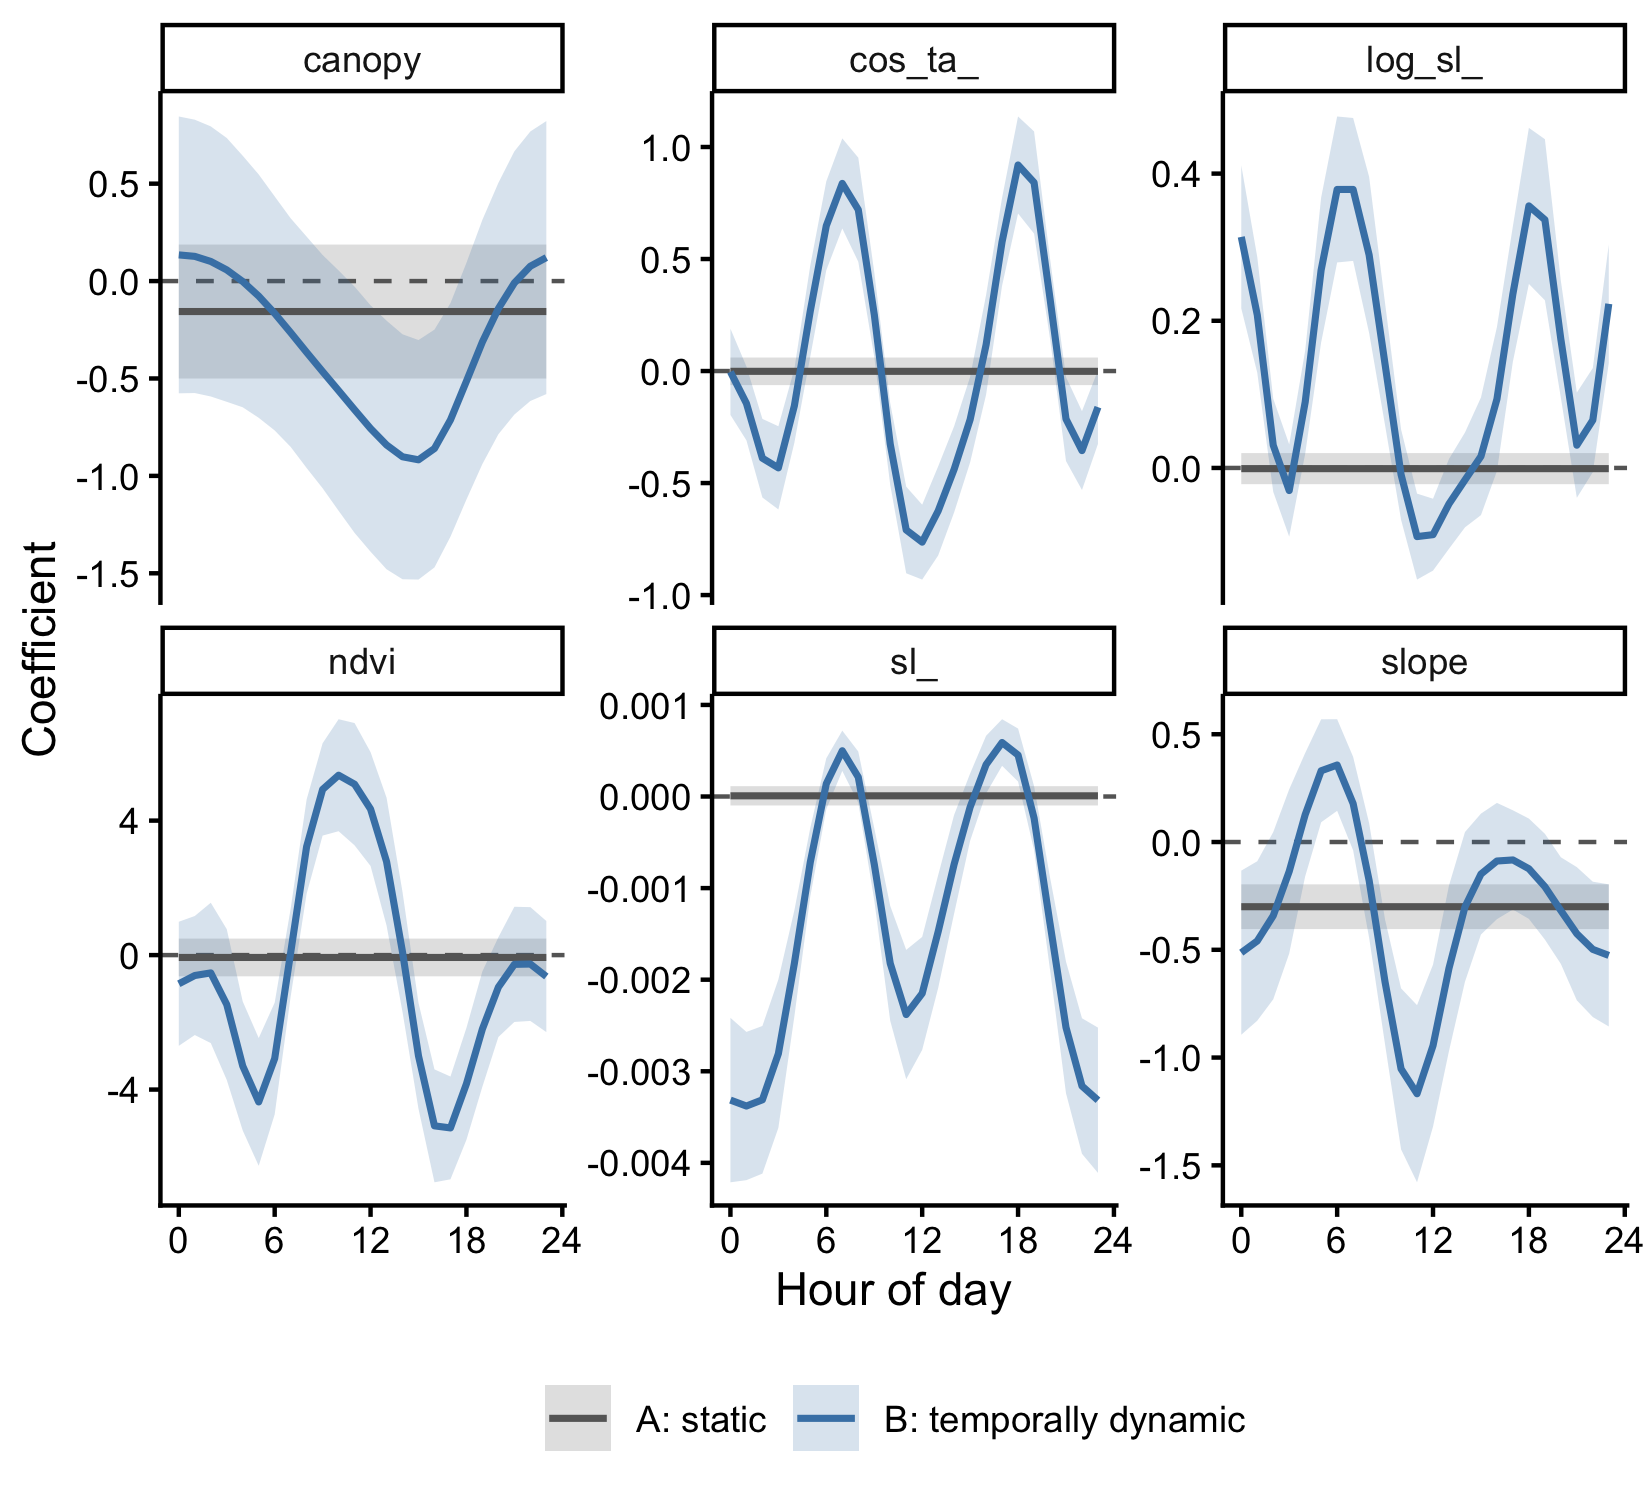
\includegraphics[keepaspectratio]{predictive_SSF_walkthrough_files/figure-pdf/plot_betas-1.png}}

}

\caption{Estimated coefficients across the day. The static model (grey)
is constant by construction; the dynamic model (blue) varies.}

\end{figure}%

This is the figure that motivates the whole exercise. The static model's
NDVI coefficient is a slightly negative constant. The dynamic model
shows that this average conceals a strong daily cycle: the animal
\emph{selects} for high NDVI around the middle of the day and
\emph{avoids} it in the late afternoon and evening. Averaging those two
opposite behaviours together produces a number that describes neither.

\subsection{Correcting the movement
parameters}\label{correcting-the-movement-parameters}

The movement coefficients are not selection coefficients --- they are
\emph{corrections} to the tentative distributions we fitted in section
3. The update rules for a gamma step-length distribution and a von Mises
turning-angle distribution are (Avgar et al. 2016; Fieberg et al. 2021):

\[
\text{shape}(\tau) = \text{shape}_{\text{tentative}} + \beta_{\log(\text{sl})}(\tau)
\] \[
\text{scale}(\tau) = \frac{1}{\ \dfrac{1}{\text{scale}_{\text{tentative}}} - \beta_{\text{sl}}(\tau)\ }
\] \[
\kappa(\tau) = \kappa_{\text{tentative}} + \beta_{\cos(\text{ta})}(\tau)
\]

\begin{Shaded}
\begin{Highlighting}[]
\CommentTok{\#\textquotesingle{} Build a 24{-}row table of hourly coefficients and movement parameters}
\NormalTok{build\_hourly\_coefs }\OtherTok{\textless{}{-}} \ControlFlowTok{function}\NormalTok{(model) \{}

\NormalTok{  betas }\OtherTok{\textless{}{-}} \FunctionTok{map\_dfr}\NormalTok{(model\_terms, }\SpecialCharTok{\textasciitilde{}} \FunctionTok{beta\_by\_hour}\NormalTok{(model, .x)) }\SpecialCharTok{\%\textgreater{}\%}
    \FunctionTok{select}\NormalTok{(hour, variable, estimate) }\SpecialCharTok{\%\textgreater{}\%}
    \FunctionTok{pivot\_wider}\NormalTok{(}\AttributeTok{names\_from =}\NormalTok{ variable, }\AttributeTok{values\_from =}\NormalTok{ estimate)}

\NormalTok{  betas }\SpecialCharTok{\%\textgreater{}\%}
    \FunctionTok{mutate}\NormalTok{(}
      \CommentTok{\# Apply the iSSA update rules to recover the corrected movement kernel}
      \AttributeTok{shape =}\NormalTok{ shape\_tentative }\SpecialCharTok{+}\NormalTok{ log\_sl\_,}
      \AttributeTok{scale =} \DecValTok{1} \SpecialCharTok{/}\NormalTok{ ((}\DecValTok{1} \SpecialCharTok{/}\NormalTok{ scale\_tentative) }\SpecialCharTok{{-}}\NormalTok{ sl\_),}
      \AttributeTok{kappa =}\NormalTok{ kappa\_tentative }\SpecialCharTok{+}\NormalTok{ cos\_ta\_}
\NormalTok{    ) }\SpecialCharTok{\%\textgreater{}\%}
    \FunctionTok{select}\NormalTok{(hour, ndvi, canopy, slope, shape, scale, kappa)}
\NormalTok{\}}

\NormalTok{hourly\_coefs\_static  }\OtherTok{\textless{}{-}} \FunctionTok{build\_hourly\_coefs}\NormalTok{(ssf\_static\_gam)}
\NormalTok{hourly\_coefs\_dynamic }\OtherTok{\textless{}{-}} \FunctionTok{build\_hourly\_coefs}\NormalTok{(ssf\_dynamic)}

\NormalTok{hourly\_coefs\_dynamic}
\end{Highlighting}
\end{Shaded}

\begin{verbatim}
# A tibble: 24 x 7
    hour    ndvi   canopy  slope shape scale    kappa
   <int>   <dbl>    <dbl>  <dbl> <dbl> <dbl>    <dbl>
 1     0 -0.854   0.134   -0.513 0.741  218.  0.395  
 2     1 -0.607   0.127   -0.459 0.635  215.  0.254  
 3     2 -0.530   0.101   -0.342 0.457  218.  0.00934
 4     3 -1.47    0.0574  -0.136 0.396  245. -0.0338 
 5     4 -3.30   -0.00228  0.127 0.516  323.  0.243  
 6     5 -4.37   -0.0772   0.331 0.696  504.  0.667  
 7     6 -3.08   -0.166    0.357 0.805  884.  1.05   
 8     7  0.0726 -0.265    0.178 0.805 1296.  1.24   
 9     8  3.23   -0.366   -0.178 0.716  944.  1.12   
10     9  4.93   -0.465   -0.650 0.567  498.  0.651  
# i 14 more rows
\end{verbatim}

\subsection{\texorpdfstring{Checking the update rules against
\texttt{amt}}{Checking the update rules against amt}}\label{checking-the-update-rules-against-amt}

These update rules are the single most important piece of arithmetic in
the script: if they are wrong, every simulated step length is wrong and
nothing downstream means anything. \texttt{amt} implements them
directly, so for the static model we can check our hand-computed values
against the package.

\begin{Shaded}
\begin{Highlighting}[]
\NormalTok{amt\_sl }\OtherTok{\textless{}{-}}\NormalTok{ amt}\SpecialCharTok{::}\FunctionTok{update\_sl\_distr}\NormalTok{(ssf\_static)}
\NormalTok{amt\_ta }\OtherTok{\textless{}{-}}\NormalTok{ amt}\SpecialCharTok{::}\FunctionTok{update\_ta\_distr}\NormalTok{(ssf\_static)}

\FunctionTok{tibble}\NormalTok{(}
  \AttributeTok{parameter =} \FunctionTok{c}\NormalTok{(}\StringTok{"shape"}\NormalTok{, }\StringTok{"scale"}\NormalTok{, }\StringTok{"kappa"}\NormalTok{),}
  \AttributeTok{manual    =} \FunctionTok{c}\NormalTok{(hourly\_coefs\_static}\SpecialCharTok{$}\NormalTok{shape[}\DecValTok{1}\NormalTok{],}
\NormalTok{                hourly\_coefs\_static}\SpecialCharTok{$}\NormalTok{scale[}\DecValTok{1}\NormalTok{],}
\NormalTok{                hourly\_coefs\_static}\SpecialCharTok{$}\NormalTok{kappa[}\DecValTok{1}\NormalTok{]),}
  \AttributeTok{amt       =} \FunctionTok{c}\NormalTok{(amt\_sl}\SpecialCharTok{$}\NormalTok{params}\SpecialCharTok{$}\NormalTok{shape, amt\_sl}\SpecialCharTok{$}\NormalTok{params}\SpecialCharTok{$}\NormalTok{scale, amt\_ta}\SpecialCharTok{$}\NormalTok{params}\SpecialCharTok{$}\NormalTok{kappa)}
\NormalTok{) }\SpecialCharTok{\%\textgreater{}\%}
  \FunctionTok{mutate}\NormalTok{(}\AttributeTok{difference =}\NormalTok{ manual }\SpecialCharTok{{-}}\NormalTok{ amt)}
\end{Highlighting}
\end{Shaded}

\begin{verbatim}
# A tibble: 3 x 4
  parameter  manual     amt difference
  <chr>       <dbl>   <dbl>      <dbl>
1 shape       0.426   0.426   8.29e-13
2 scale     791.    791.      4.68e- 9
3 kappa       0.397   0.397  -5.11e-13
\end{verbatim}

Identical. We can trust the hourly tables.

\begin{Shaded}
\begin{Highlighting}[]
\FunctionTok{bind\_rows}\NormalTok{(}
\NormalTok{  hourly\_coefs\_static  }\SpecialCharTok{\%\textgreater{}\%} \FunctionTok{mutate}\NormalTok{(}\AttributeTok{model =} \StringTok{"A: static"}\NormalTok{),}
\NormalTok{  hourly\_coefs\_dynamic }\SpecialCharTok{\%\textgreater{}\%} \FunctionTok{mutate}\NormalTok{(}\AttributeTok{model =} \StringTok{"B: temporally dynamic"}\NormalTok{)}
\NormalTok{) }\SpecialCharTok{\%\textgreater{}\%}
  \FunctionTok{mutate}\NormalTok{(}\StringTok{\textasciigrave{}}\AttributeTok{mean step length (m)}\StringTok{\textasciigrave{}} \OtherTok{=}\NormalTok{ shape }\SpecialCharTok{*}\NormalTok{ scale) }\SpecialCharTok{\%\textgreater{}\%}
  \FunctionTok{select}\NormalTok{(hour, model, shape, scale, kappa, }\StringTok{\textasciigrave{}}\AttributeTok{mean step length (m)}\StringTok{\textasciigrave{}}\NormalTok{) }\SpecialCharTok{\%\textgreater{}\%}
  \FunctionTok{pivot\_longer}\NormalTok{(}\FunctionTok{c}\NormalTok{(shape, scale, kappa, }\StringTok{\textasciigrave{}}\AttributeTok{mean step length (m)}\StringTok{\textasciigrave{}}\NormalTok{),}
               \AttributeTok{names\_to =} \StringTok{"parameter"}\NormalTok{, }\AttributeTok{values\_to =} \StringTok{"value"}\NormalTok{) }\SpecialCharTok{\%\textgreater{}\%}
  \FunctionTok{ggplot}\NormalTok{(}\FunctionTok{aes}\NormalTok{(}\AttributeTok{x =}\NormalTok{ hour, }\AttributeTok{y =}\NormalTok{ value, }\AttributeTok{colour =}\NormalTok{ model)) }\SpecialCharTok{+}
  \FunctionTok{geom\_line}\NormalTok{(}\AttributeTok{linewidth =} \FloatTok{0.8}\NormalTok{) }\SpecialCharTok{+}
  \FunctionTok{facet\_wrap}\NormalTok{(}\SpecialCharTok{\textasciitilde{}}\NormalTok{ parameter, }\AttributeTok{scales =} \StringTok{"free\_y"}\NormalTok{, }\AttributeTok{nrow =} \DecValTok{1}\NormalTok{) }\SpecialCharTok{+}
  \FunctionTok{scale\_colour\_manual}\NormalTok{(}\AttributeTok{values =} \FunctionTok{c}\NormalTok{(}\StringTok{"A: static"} \OtherTok{=} \StringTok{"grey40"}\NormalTok{,}
                                 \StringTok{"B: temporally dynamic"} \OtherTok{=} \StringTok{"steelblue"}\NormalTok{), }\AttributeTok{name =} \ConstantTok{NULL}\NormalTok{) }\SpecialCharTok{+}
  \FunctionTok{scale\_x\_continuous}\NormalTok{(}\StringTok{"Hour of day"}\NormalTok{, }\AttributeTok{breaks =} \FunctionTok{seq}\NormalTok{(}\DecValTok{0}\NormalTok{, }\DecValTok{24}\NormalTok{, }\DecValTok{6}\NormalTok{)) }\SpecialCharTok{+}
  \FunctionTok{labs}\NormalTok{(}\AttributeTok{y =} \ConstantTok{NULL}\NormalTok{) }\SpecialCharTok{+}
  \FunctionTok{theme\_classic}\NormalTok{() }\SpecialCharTok{+}
  \FunctionTok{theme}\NormalTok{(}\AttributeTok{legend.position =} \StringTok{"bottom"}\NormalTok{)}
\end{Highlighting}
\end{Shaded}

\begin{figure}[H]

{\centering \pandocbounded{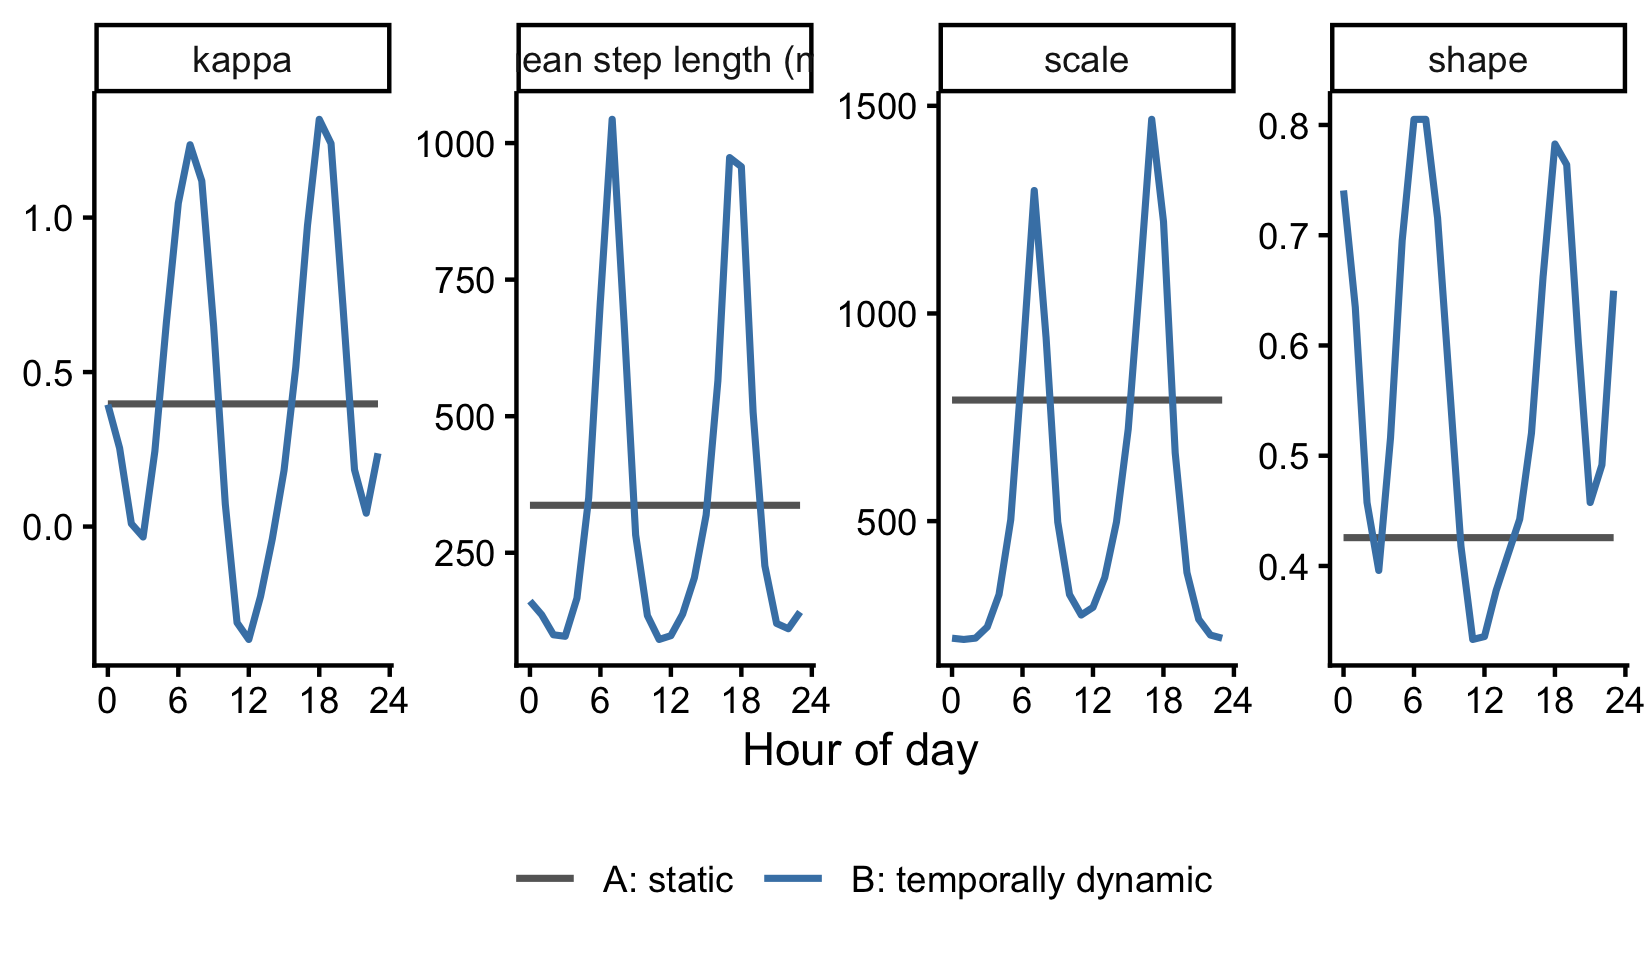
\includegraphics[keepaspectratio]{predictive_SSF_walkthrough_files/figure-pdf/plot_movement_params-1.png}}

}

\caption{Corrected movement parameters across the day. Mean step length
is the product of shape and scale.}

\end{figure}%

The dynamic model recovers a clear daily activity cycle: short steps
through the middle of the day (resting) and long, directed steps in the
early evening. The static model, by construction, has the animal moving
the same way at every hour.

\begin{tcolorbox}[enhanced jigsaw, arc=.35mm, bottomrule=.15mm, bottomtitle=1mm, breakable, colback=white, colbacktitle=quarto-callout-note-color!10!white, colframe=quarto-callout-note-color-frame, coltitle=black, left=2mm, leftrule=.75mm, opacityback=0, opacitybacktitle=0.6, rightrule=.15mm, title=\textcolor{quarto-callout-note-color}{\faInfo}\hspace{0.5em}{Check that the corrected parameters are valid}, titlerule=0mm, toprule=.15mm, toptitle=1mm]

The update rules involve a subtraction, so it is possible in principle
for them to produce an invalid distribution --- a negative shape, or a
negative scale if
\(\beta_{\text{sl}}(\tau) > 1/\text{scale}_{\text{tentative}}\). It is
worth checking explicitly before simulating, rather than discovering it
as an obscure error inside the simulation loop.

\end{tcolorbox}

\begin{Shaded}
\begin{Highlighting}[]
\NormalTok{hourly\_coefs\_dynamic }\SpecialCharTok{\%\textgreater{}\%}
  \FunctionTok{summarise}\NormalTok{(}
    \AttributeTok{min\_shape       =} \FunctionTok{min}\NormalTok{(shape),}
    \AttributeTok{min\_scale       =} \FunctionTok{min}\NormalTok{(scale),}
    \AttributeTok{shape\_all\_valid =} \FunctionTok{all}\NormalTok{(shape }\SpecialCharTok{\textgreater{}} \DecValTok{0}\NormalTok{),}
    \AttributeTok{scale\_all\_valid =} \FunctionTok{all}\NormalTok{(scale }\SpecialCharTok{\textgreater{}} \DecValTok{0}\NormalTok{),}
    \AttributeTok{kappa\_range     =} \FunctionTok{paste}\NormalTok{(}\FunctionTok{round}\NormalTok{(}\FunctionTok{range}\NormalTok{(kappa), }\DecValTok{3}\NormalTok{), }\AttributeTok{collapse =} \StringTok{" to "}\NormalTok{)}
\NormalTok{  )}
\end{Highlighting}
\end{Shaded}

\begin{verbatim}
# A tibble: 1 x 5
  min_shape min_scale shape_all_valid scale_all_valid kappa_range    
      <dbl>     <dbl> <lgl>           <lgl>           <chr>          
1     0.333      215. TRUE            TRUE            -0.365 to 1.318
\end{verbatim}

\section{7. Pre-computing hourly habitat selection
surfaces}\label{pre-computing-hourly-habitat-selection-surfaces}

For the simulation we need, at every candidate step, the value of the
habitat selection function

\[
\log \omega(\mathbf{X}(s); \boldsymbol{\beta}(\tau)) = \beta_{\text{NDVI}}(\tau)\,\text{NDVI}(s) + \beta_{\text{canopy}}(\tau)\,\text{canopy}(s) + \beta_{\text{slope}}(\tau)\,\text{slope}(s)
\]

Rather than evaluating this at each of the millions of candidate steps
we will generate, we compute it \textbf{once per hour} across the whole
landscape, producing a 24-layer raster stack. The simulation then just
looks up a value. We keep everything on the log scale and exponentiate
only when sampling, which is both faster and numerically safer.

\begin{Shaded}
\begin{Highlighting}[]
\CommentTok{\#\textquotesingle{} Build a 24{-}layer raster stack of log habitat selection values, one per hour}
\NormalTok{build\_hourly\_surfaces }\OtherTok{\textless{}{-}} \ControlFlowTok{function}\NormalTok{(hourly\_coefs) \{}

\NormalTok{  layers }\OtherTok{\textless{}{-}} \FunctionTok{map}\NormalTok{(}\DecValTok{1}\SpecialCharTok{:}\DecValTok{24}\NormalTok{, }\ControlFlowTok{function}\NormalTok{(i) \{}
\NormalTok{    cf }\OtherTok{\textless{}{-}}\NormalTok{ hourly\_coefs[i, ]}
    \CommentTok{\# Linear predictor for this hour, across the whole landscape}
\NormalTok{    ndvi\_crop }\SpecialCharTok{*}\NormalTok{ cf}\SpecialCharTok{$}\NormalTok{ndvi }\SpecialCharTok{+}\NormalTok{ canopy\_crop }\SpecialCharTok{*}\NormalTok{ cf}\SpecialCharTok{$}\NormalTok{canopy }\SpecialCharTok{+}\NormalTok{ slope\_crop }\SpecialCharTok{*}\NormalTok{ cf}\SpecialCharTok{$}\NormalTok{slope}
\NormalTok{  \})}

\NormalTok{  stk }\OtherTok{\textless{}{-}} \FunctionTok{rast}\NormalTok{(layers)}
  \FunctionTok{names}\NormalTok{(stk) }\OtherTok{\textless{}{-}} \FunctionTok{paste0}\NormalTok{(}\StringTok{"hour\_"}\NormalTok{, hourly\_coefs}\SpecialCharTok{$}\NormalTok{hour)}
\NormalTok{  stk}
\NormalTok{\}}

\FunctionTok{tic}\NormalTok{(}\StringTok{"Building hourly selection surfaces"}\NormalTok{)}
\NormalTok{surfaces\_static  }\OtherTok{\textless{}{-}} \FunctionTok{build\_hourly\_surfaces}\NormalTok{(hourly\_coefs\_static)}
\NormalTok{surfaces\_dynamic }\OtherTok{\textless{}{-}} \FunctionTok{build\_hourly\_surfaces}\NormalTok{(hourly\_coefs\_dynamic)}
\FunctionTok{toc}\NormalTok{()}
\end{Highlighting}
\end{Shaded}

\begin{verbatim}
Building hourly selection surfaces: 0.588 sec elapsed
\end{verbatim}

\begin{Shaded}
\begin{Highlighting}[]
\NormalTok{surfaces\_dynamic}
\end{Highlighting}
\end{Shaded}

\begin{verbatim}
class       : SpatRaster
size        : 560, 560, 24  (nrow, ncol, nlyr)
resolution  : 25, 25  (x, y)
extent      : 17000, 31000, -1440000, -1426000  (xmin, xmax, ymin, ymax)
coord. ref. : GDA94 / Geoscience Australia Lambert (EPSG:3112)
source(s)   : memory
names       :    hour_0,    hour_1,    hour_2,    hour_3,    hour_4,    hour_5, ...
min values  : -3.170461, -2.788128, -2.096492, -1.352342, -2.509994, -3.366588, ...
max values  :  0.073107,  0.056587,  0.044605,   0.15044,  0.504934,  0.994433, ...
\end{verbatim}

\begin{Shaded}
\begin{Highlighting}[]
\CommentTok{\# A shared, symmetric colour scale so the panels are comparable}
\NormalTok{sel\_range }\OtherTok{\textless{}{-}} \FunctionTok{range}\NormalTok{(}\FunctionTok{c}\NormalTok{(}\FunctionTok{values}\NormalTok{(surfaces\_dynamic), }\FunctionTok{values}\NormalTok{(surfaces\_static)), }\AttributeTok{na.rm =} \ConstantTok{TRUE}\NormalTok{)}
\NormalTok{sel\_max   }\OtherTok{\textless{}{-}} \FunctionTok{max}\NormalTok{(}\FunctionTok{abs}\NormalTok{(sel\_range))}

\NormalTok{plot\_hours }\OtherTok{\textless{}{-}} \FunctionTok{c}\NormalTok{(}\DecValTok{3}\NormalTok{, }\DecValTok{9}\NormalTok{, }\DecValTok{15}\NormalTok{, }\DecValTok{21}\NormalTok{)}

\FunctionTok{par}\NormalTok{(}\AttributeTok{mfrow =} \FunctionTok{c}\NormalTok{(}\DecValTok{2}\NormalTok{, }\DecValTok{4}\NormalTok{), }\AttributeTok{mar =} \FunctionTok{c}\NormalTok{(}\DecValTok{2}\NormalTok{, }\DecValTok{2}\NormalTok{, }\DecValTok{3}\NormalTok{, }\DecValTok{4}\NormalTok{))}
\ControlFlowTok{for}\NormalTok{ (h }\ControlFlowTok{in}\NormalTok{ plot\_hours) \{}
  \FunctionTok{plot}\NormalTok{(surfaces\_static[[h }\SpecialCharTok{+} \DecValTok{1}\NormalTok{]], }\AttributeTok{main =} \FunctionTok{paste0}\NormalTok{(}\StringTok{"Static, "}\NormalTok{, h, }\StringTok{":00"}\NormalTok{),}
       \AttributeTok{range =} \FunctionTok{c}\NormalTok{(}\SpecialCharTok{{-}}\NormalTok{sel\_max, sel\_max), }\AttributeTok{col =} \FunctionTok{brewer.pal}\NormalTok{(}\DecValTok{11}\NormalTok{, }\StringTok{"RdBu"}\NormalTok{))}
\NormalTok{\}}
\ControlFlowTok{for}\NormalTok{ (h }\ControlFlowTok{in}\NormalTok{ plot\_hours) \{}
  \FunctionTok{plot}\NormalTok{(surfaces\_dynamic[[h }\SpecialCharTok{+} \DecValTok{1}\NormalTok{]], }\AttributeTok{main =} \FunctionTok{paste0}\NormalTok{(}\StringTok{"Dynamic, "}\NormalTok{, h, }\StringTok{":00"}\NormalTok{),}
       \AttributeTok{range =} \FunctionTok{c}\NormalTok{(}\SpecialCharTok{{-}}\NormalTok{sel\_max, sel\_max), }\AttributeTok{col =} \FunctionTok{brewer.pal}\NormalTok{(}\DecValTok{11}\NormalTok{, }\StringTok{"RdBu"}\NormalTok{))}
\NormalTok{\}}
\end{Highlighting}
\end{Shaded}

\begin{figure}[H]

{\centering \pandocbounded{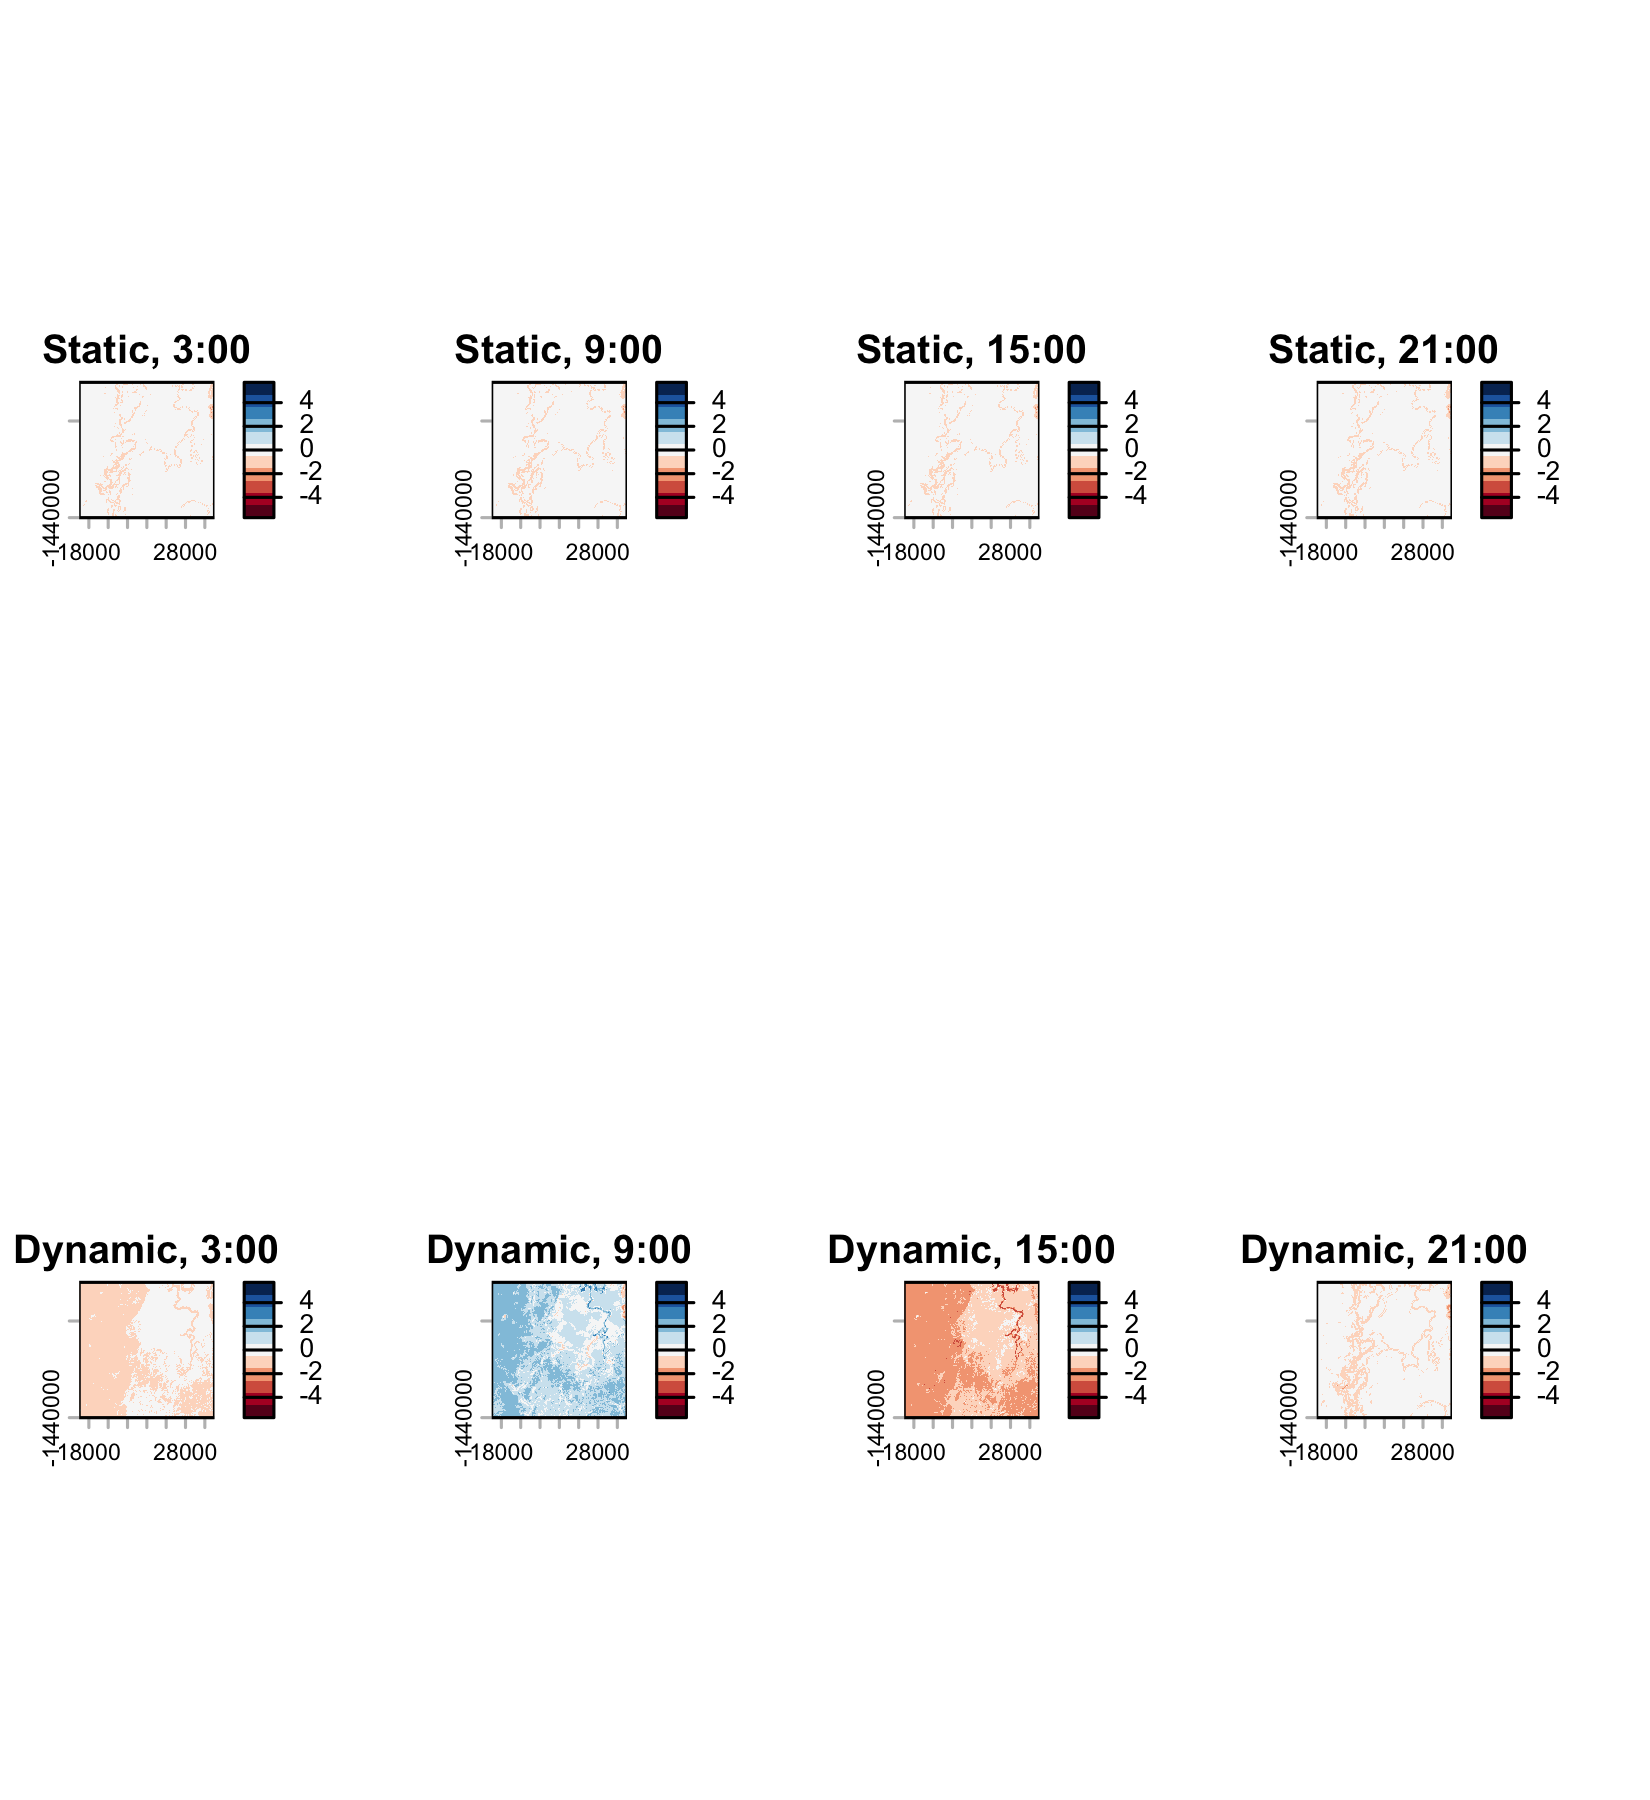
\includegraphics[keepaspectratio]{predictive_SSF_walkthrough_files/figure-pdf/plot_surfaces-1.png}}

}

\caption{Log habitat selection surfaces at four times of day. The static
model is identical at every hour; the dynamic model changes markedly.}

\end{figure}%

\begin{Shaded}
\begin{Highlighting}[]
\FunctionTok{par}\NormalTok{(}\AttributeTok{mfrow =} \FunctionTok{c}\NormalTok{(}\DecValTok{1}\NormalTok{, }\DecValTok{1}\NormalTok{))}
\end{Highlighting}
\end{Shaded}

\subsection{An animation of the daily
cycle}\label{an-animation-of-the-daily-cycle}

The daily cycle is much easier to appreciate as an animation than as
four static panels.

\begin{Shaded}
\begin{Highlighting}[]
\NormalTok{surface\_gif\_path }\OtherTok{\textless{}{-}} \FunctionTok{file.path}\NormalTok{(plot\_save\_path, }\StringTok{"hourly\_selection\_surfaces.gif"}\NormalTok{)}

\CommentTok{\# Render one frame per hour, all on the same colour scale so that the animation}
\CommentTok{\# shows genuine change rather than rescaling}
\NormalTok{frame\_files }\OtherTok{\textless{}{-}} \FunctionTok{map\_chr}\NormalTok{(}\DecValTok{0}\SpecialCharTok{:}\DecValTok{23}\NormalTok{, }\ControlFlowTok{function}\NormalTok{(h) \{}
\NormalTok{  f }\OtherTok{\textless{}{-}} \FunctionTok{file.path}\NormalTok{(plot\_save\_path, }\FunctionTok{sprintf}\NormalTok{(}\StringTok{"surface\_frame\_\%02d.png"}\NormalTok{, h))}
  \FunctionTok{png}\NormalTok{(f, }\AttributeTok{width =} \DecValTok{110}\NormalTok{, }\AttributeTok{height =} \DecValTok{110}\NormalTok{, }\AttributeTok{units =} \StringTok{"mm"}\NormalTok{, }\AttributeTok{res =} \DecValTok{150}\NormalTok{)}
  \FunctionTok{plot}\NormalTok{(surfaces\_dynamic[[h }\SpecialCharTok{+} \DecValTok{1}\NormalTok{]],}
       \AttributeTok{main =} \FunctionTok{sprintf}\NormalTok{(}\StringTok{"Habitat selection, \%02d:00"}\NormalTok{, h),}
       \AttributeTok{range =} \FunctionTok{c}\NormalTok{(}\SpecialCharTok{{-}}\NormalTok{sel\_max, sel\_max), }\AttributeTok{col =} \FunctionTok{brewer.pal}\NormalTok{(}\DecValTok{11}\NormalTok{, }\StringTok{"RdBu"}\NormalTok{))}
  \FunctionTok{dev.off}\NormalTok{()}
\NormalTok{  f}
\NormalTok{\})}

\FunctionTok{image\_read}\NormalTok{(frame\_files) }\SpecialCharTok{\%\textgreater{}\%}
  \FunctionTok{image\_animate}\NormalTok{(}\AttributeTok{fps =} \DecValTok{4}\NormalTok{) }\SpecialCharTok{\%\textgreater{}\%}
  \FunctionTok{image\_write}\NormalTok{(surface\_gif\_path)}

\CommentTok{\# Tidy up the individual frames}
\FunctionTok{unlink}\NormalTok{(frame\_files)}
\end{Highlighting}
\end{Shaded}

\begin{figure}[H]

{\centering \pandocbounded{\includegraphics[keepaspectratio]{outputs/walkthrough/hourly_selection_surfaces.gif}}

}

\caption{Hourly habitat selection surfaces under the temporally dynamic
model.}

\end{figure}%

\section{8. Simulating trajectories}\label{simulating-trajectories}

\subsection{The redistribution kernel}\label{the-redistribution-kernel}

Simulating from a fitted SSF means repeatedly sampling the next location
from a \textbf{redistribution kernel}, which is the product of two
parts:

\[
\underbrace{\phi(s' \mid s, \tau)}_{\text{movement kernel}} \times \underbrace{\omega(\mathbf{X}(s'); \boldsymbol{\beta}(\tau))}_{\text{habitat kernel}}
\]

In practice we approximate this by sampling: propose 25 candidate steps
from the movement kernel, weight each by its habitat value, and choose
one with probability proportional to that weight. This is exactly the
structure of the model we fitted --- the same conditional-logistic
machinery, run forwards instead of backwards.

\subsection{A fast raster lookup}\label{a-fast-raster-lookup}

The simulation needs tens of millions of raster lookups.
\texttt{terra::extract()} is convenient but carries a per-call overhead
that dominates when it is called hundreds of thousands of times, so we
extract the raster values into a plain matrix once, and index into it
with arithmetic.

\begin{Shaded}
\begin{Highlighting}[]
\CommentTok{\#\textquotesingle{} Pre{-}digest a raster stack into a plain matrix plus its geometry}
\CommentTok{\#\textquotesingle{}}
\CommentTok{\#\textquotesingle{} \textasciigrave{}terra::values()\textasciigrave{} returns a matrix with one row per cell (in row{-}major order)}
\CommentTok{\#\textquotesingle{} and one column per layer, which is exactly what we need for fast indexing.}
\NormalTok{prepare\_lookup }\OtherTok{\textless{}{-}} \ControlFlowTok{function}\NormalTok{(stk) \{}
  \FunctionTok{list}\NormalTok{(}\AttributeTok{vals =}\NormalTok{ terra}\SpecialCharTok{::}\FunctionTok{values}\NormalTok{(stk),}
       \AttributeTok{xmin =} \FunctionTok{xmin}\NormalTok{(stk), }\AttributeTok{ymax =} \FunctionTok{ymax}\NormalTok{(stk),}
       \AttributeTok{nrow =} \FunctionTok{nrow}\NormalTok{(stk), }\AttributeTok{ncol =} \FunctionTok{ncol}\NormalTok{(stk),}
       \AttributeTok{resx =} \FunctionTok{res}\NormalTok{(stk)[}\DecValTok{1}\NormalTok{], }\AttributeTok{resy =} \FunctionTok{res}\NormalTok{(stk)[}\DecValTok{2}\NormalTok{])}
\NormalTok{\}}

\CommentTok{\#\textquotesingle{} Look up values at coordinates in a given layer}
\CommentTok{\#\textquotesingle{}}
\CommentTok{\#\textquotesingle{} Equivalent to \textasciigrave{}terra::extract(stk[[layer]], cbind(x, y))[, 1]\textasciigrave{}, but without the}
\CommentTok{\#\textquotesingle{} per{-}call overhead. Coordinates outside the raster return NA.}
\NormalTok{lookup }\OtherTok{\textless{}{-}} \ControlFlowTok{function}\NormalTok{(lk, x, y, layer) \{}
\NormalTok{  col }\OtherTok{\textless{}{-}} \FunctionTok{floor}\NormalTok{((x }\SpecialCharTok{{-}}\NormalTok{ lk}\SpecialCharTok{$}\NormalTok{xmin) }\SpecialCharTok{/}\NormalTok{ lk}\SpecialCharTok{$}\NormalTok{resx) }\SpecialCharTok{+} \DecValTok{1}
\NormalTok{  row }\OtherTok{\textless{}{-}} \FunctionTok{floor}\NormalTok{((lk}\SpecialCharTok{$}\NormalTok{ymax }\SpecialCharTok{{-}}\NormalTok{ y) }\SpecialCharTok{/}\NormalTok{ lk}\SpecialCharTok{$}\NormalTok{resy) }\SpecialCharTok{+} \DecValTok{1}

  \CommentTok{\# \textasciigrave{}\%in\%\textasciigrave{}{-}style guard: a non{-}finite coordinate is not inside the raster. Without}
  \CommentTok{\# \textasciigrave{}isTRUE\textasciigrave{}{-}style handling, a NaN coordinate would make \textasciigrave{}inside\textasciigrave{} NA rather than}
  \CommentTok{\# FALSE, and NA is not permitted as a subscript in the assignment below.}
\NormalTok{  inside }\OtherTok{\textless{}{-}} \SpecialCharTok{!}\FunctionTok{is.na}\NormalTok{(col) }\SpecialCharTok{\&} \SpecialCharTok{!}\FunctionTok{is.na}\NormalTok{(row) }\SpecialCharTok{\&}
\NormalTok{    col }\SpecialCharTok{\textgreater{}=} \DecValTok{1} \SpecialCharTok{\&}\NormalTok{ col }\SpecialCharTok{\textless{}=}\NormalTok{ lk}\SpecialCharTok{$}\NormalTok{ncol }\SpecialCharTok{\&}\NormalTok{ row }\SpecialCharTok{\textgreater{}=} \DecValTok{1} \SpecialCharTok{\&}\NormalTok{ row }\SpecialCharTok{\textless{}=}\NormalTok{ lk}\SpecialCharTok{$}\NormalTok{nrow}

\NormalTok{  out }\OtherTok{\textless{}{-}} \FunctionTok{rep}\NormalTok{(}\ConstantTok{NA\_real\_}\NormalTok{, }\FunctionTok{length}\NormalTok{(x))}
\NormalTok{  cell }\OtherTok{\textless{}{-}}\NormalTok{ (row[inside] }\SpecialCharTok{{-}} \DecValTok{1}\NormalTok{) }\SpecialCharTok{*}\NormalTok{ lk}\SpecialCharTok{$}\NormalTok{ncol }\SpecialCharTok{+}\NormalTok{ col[inside]}
\NormalTok{  out[inside] }\OtherTok{\textless{}{-}}\NormalTok{ lk}\SpecialCharTok{$}\NormalTok{vals[cell, layer]}
\NormalTok{  out}
\NormalTok{\}}
\end{Highlighting}
\end{Shaded}

\begin{Shaded}
\begin{Highlighting}[]
\CommentTok{\# Confirm the fast lookup agrees with terra on a sample of points}
\NormalTok{check\_x }\OtherTok{\textless{}{-}} \FunctionTok{runif}\NormalTok{(}\DecValTok{1000}\NormalTok{, }\FunctionTok{xmin}\NormalTok{(surfaces\_dynamic), }\FunctionTok{xmax}\NormalTok{(surfaces\_dynamic))}
\NormalTok{check\_y }\OtherTok{\textless{}{-}} \FunctionTok{runif}\NormalTok{(}\DecValTok{1000}\NormalTok{, }\FunctionTok{ymin}\NormalTok{(surfaces\_dynamic), }\FunctionTok{ymax}\NormalTok{(surfaces\_dynamic))}

\NormalTok{lk\_check   }\OtherTok{\textless{}{-}} \FunctionTok{prepare\_lookup}\NormalTok{(surfaces\_dynamic)}
\NormalTok{fast\_vals  }\OtherTok{\textless{}{-}} \FunctionTok{lookup}\NormalTok{(lk\_check, check\_x, check\_y, }\DecValTok{12}\NormalTok{)}
\NormalTok{terra\_vals }\OtherTok{\textless{}{-}}\NormalTok{ terra}\SpecialCharTok{::}\FunctionTok{extract}\NormalTok{(surfaces\_dynamic[[}\DecValTok{12}\NormalTok{]], }\FunctionTok{cbind}\NormalTok{(check\_x, check\_y))[, }\DecValTok{1}\NormalTok{]}

\FunctionTok{cat}\NormalTok{(}\StringTok{"Maximum absolute difference:"}\NormalTok{,}
    \FunctionTok{max}\NormalTok{(}\FunctionTok{abs}\NormalTok{(fast\_vals }\SpecialCharTok{{-}}\NormalTok{ terra\_vals), }\AttributeTok{na.rm =} \ConstantTok{TRUE}\NormalTok{), }\StringTok{"}\SpecialCharTok{\textbackslash{}n}\StringTok{"}\NormalTok{)}
\end{Highlighting}
\end{Shaded}

\begin{verbatim}
Maximum absolute difference: 0 
\end{verbatim}

\begin{Shaded}
\begin{Highlighting}[]
\FunctionTok{cat}\NormalTok{(}\StringTok{"NA agreement:"}\NormalTok{, }\FunctionTok{all}\NormalTok{(}\FunctionTok{is.na}\NormalTok{(fast\_vals) }\SpecialCharTok{==} \FunctionTok{is.na}\NormalTok{(terra\_vals)), }\StringTok{"}\SpecialCharTok{\textbackslash{}n}\StringTok{"}\NormalTok{)}
\end{Highlighting}
\end{Shaded}

\begin{verbatim}
NA agreement: TRUE 
\end{verbatim}

\subsection{The simulation function}\label{the-simulation-function}

\begin{Shaded}
\begin{Highlighting}[]
\CommentTok{\#\textquotesingle{} Simulate a single trajectory from a fitted step selection function}
\CommentTok{\#\textquotesingle{}}
\CommentTok{\#\textquotesingle{} @param n\_steps  number of steps to simulate}
\CommentTok{\#\textquotesingle{} @param n\_ch     number of candidate steps proposed at each step}
\CommentTok{\#\textquotesingle{} @param coefs    24{-}row table of hourly coefficients and movement parameters}
\CommentTok{\#\textquotesingle{} @param xy0      starting location, as c(x, y), on the shifted (origin at 0,0) grid}
\CommentTok{\#\textquotesingle{} @param lk       lookup object from \textasciigrave{}prepare\_lookup()\textasciigrave{}}
\CommentTok{\#\textquotesingle{} @param boundary "wrapped" (toroidal) or "reflective"}
\CommentTok{\#\textquotesingle{} @param start\_hour hour of day at which the trajectory begins}
\CommentTok{\#\textquotesingle{}}
\CommentTok{\#\textquotesingle{} @return a data frame with one row per step}
\NormalTok{simulate\_ssf }\OtherTok{\textless{}{-}} \ControlFlowTok{function}\NormalTok{(n\_steps, n\_ch, coefs, xy0, lk,}
                         \AttributeTok{boundary =} \StringTok{"wrapped"}\NormalTok{, }\AttributeTok{start\_hour =} \DecValTok{0}\NormalTok{) \{}

  \CommentTok{\# Landscape dimensions, used for the wrapped boundary}
\NormalTok{  x\_extent }\OtherTok{\textless{}{-}}\NormalTok{ lk}\SpecialCharTok{$}\NormalTok{ncol }\SpecialCharTok{*}\NormalTok{ lk}\SpecialCharTok{$}\NormalTok{resx}
\NormalTok{  y\_extent }\OtherTok{\textless{}{-}}\NormalTok{ lk}\SpecialCharTok{$}\NormalTok{nrow }\SpecialCharTok{*}\NormalTok{ lk}\SpecialCharTok{$}\NormalTok{resy}

  \CommentTok{\# {-}{-}{-} Pre{-}draw all the random numbers {-}{-}{-}{-}{-}{-}{-}{-}{-}{-}{-}{-}{-}{-}{-}{-}{-}{-}{-}{-}{-}{-}{-}{-}{-}{-}{-}{-}{-}{-}{-}{-}{-}{-}{-}}
  \CommentTok{\# Drawing all step lengths and turning angles up front is far faster than}
  \CommentTok{\# drawing them one step at a time inside the loop.}

  \CommentTok{\# Which hour each step occurs in (1{-}24, indexing into \textasciigrave{}coefs\textasciigrave{})}
\NormalTok{  step\_hours }\OtherTok{\textless{}{-}}\NormalTok{ ((start\_hour }\SpecialCharTok{+} \FunctionTok{seq\_len}\NormalTok{(n\_steps) }\SpecialCharTok{{-}} \DecValTok{1}\NormalTok{) }\SpecialCharTok{\%\%} \DecValTok{24}\NormalTok{) }\SpecialCharTok{+} \DecValTok{1}

  \CommentTok{\# Step lengths: gamma, with hour{-}specific shape and scale}
\NormalTok{  sl }\OtherTok{\textless{}{-}} \FunctionTok{rgamma}\NormalTok{(n\_steps }\SpecialCharTok{*}\NormalTok{ n\_ch,}
               \AttributeTok{shape =} \FunctionTok{rep}\NormalTok{(coefs}\SpecialCharTok{$}\NormalTok{shape[step\_hours], }\AttributeTok{each =}\NormalTok{ n\_ch),}
               \AttributeTok{scale =} \FunctionTok{rep}\NormalTok{(coefs}\SpecialCharTok{$}\NormalTok{scale[step\_hours], }\AttributeTok{each =}\NormalTok{ n\_ch))}

  \CommentTok{\# Turning angles: von Mises, with hour{-}specific concentration.}
  \CommentTok{\# A positive kappa means directional persistence (angles concentrated around 0),}
  \CommentTok{\# a negative kappa means a tendency to reverse (angles concentrated around pi).}
  \CommentTok{\# \textasciigrave{}rvonmises\textasciigrave{} returns angles on [0, 2*pi), so we draw around \textasciigrave{}mu\textasciigrave{} and subtract}
  \CommentTok{\# pi to get angles on [{-}pi, pi).}
  \CommentTok{\#}
  \CommentTok{\# Only 24 distinct concentrations occur, so rather than drawing step by step we}
  \CommentTok{\# draw all the angles for each hour in one call and scatter them into position.}
  \CommentTok{\# \textasciigrave{}outer()\textasciigrave{} builds the destination indices: for step i the candidates occupy}
  \CommentTok{\# positions ((i {-} 1) * n\_ch + 1) to (i * n\_ch).}
\NormalTok{  ta }\OtherTok{\textless{}{-}} \FunctionTok{numeric}\NormalTok{(n\_steps }\SpecialCharTok{*}\NormalTok{ n\_ch)}
  \ControlFlowTok{for}\NormalTok{ (h }\ControlFlowTok{in} \FunctionTok{unique}\NormalTok{(step\_hours)) \{}
\NormalTok{    steps\_h }\OtherTok{\textless{}{-}} \FunctionTok{which}\NormalTok{(step\_hours }\SpecialCharTok{==}\NormalTok{ h)}
\NormalTok{    kappa\_h }\OtherTok{\textless{}{-}}\NormalTok{ coefs}\SpecialCharTok{$}\NormalTok{kappa[h]}
\NormalTok{    mu\_h    }\OtherTok{\textless{}{-}} \ControlFlowTok{if}\NormalTok{ (kappa\_h }\SpecialCharTok{\textgreater{}} \DecValTok{0}\NormalTok{) pi }\ControlFlowTok{else} \DecValTok{0}

\NormalTok{    ta[}\FunctionTok{as.vector}\NormalTok{(}\FunctionTok{outer}\NormalTok{(}\FunctionTok{seq\_len}\NormalTok{(n\_ch), (steps\_h }\SpecialCharTok{{-}} \DecValTok{1}\NormalTok{) }\SpecialCharTok{*}\NormalTok{ n\_ch, }\StringTok{"+"}\NormalTok{))] }\OtherTok{\textless{}{-}}
      \FunctionTok{as.numeric}\NormalTok{(circular}\SpecialCharTok{::}\FunctionTok{rvonmises}\NormalTok{(}\AttributeTok{n     =} \FunctionTok{length}\NormalTok{(steps\_h) }\SpecialCharTok{*}\NormalTok{ n\_ch,}
                                     \AttributeTok{mu    =}\NormalTok{ circular}\SpecialCharTok{::}\FunctionTok{circular}\NormalTok{(mu\_h),}
                                     \AttributeTok{kappa =} \FunctionTok{abs}\NormalTok{(kappa\_h))) }\SpecialCharTok{{-}}\NormalTok{ pi}
\NormalTok{  \}}

  \CommentTok{\# {-}{-}{-} Storage {-}{-}{-}{-}{-}{-}{-}{-}{-}{-}{-}{-}{-}{-}{-}{-}{-}{-}{-}{-}{-}{-}{-}{-}{-}{-}{-}{-}{-}{-}{-}{-}{-}{-}{-}{-}{-}{-}{-}{-}{-}{-}{-}{-}{-}{-}{-}{-}{-}{-}{-}{-}{-}{-}{-}{-}{-}{-}{-}{-}}
\NormalTok{  x }\OtherTok{\textless{}{-}}\NormalTok{ y }\OtherTok{\textless{}{-}}\NormalTok{ step\_length }\OtherTok{\textless{}{-}}\NormalTok{ angle }\OtherTok{\textless{}{-}}\NormalTok{ bearing }\OtherTok{\textless{}{-}}\NormalTok{ hab\_p }\OtherTok{\textless{}{-}} \FunctionTok{rep}\NormalTok{(}\ConstantTok{NA\_real\_}\NormalTok{, n\_steps)}

\NormalTok{  x[}\DecValTok{1}\NormalTok{] }\OtherTok{\textless{}{-}}\NormalTok{ xy0[}\DecValTok{1}\NormalTok{]}
\NormalTok{  y[}\DecValTok{1}\NormalTok{] }\OtherTok{\textless{}{-}}\NormalTok{ xy0[}\DecValTok{2}\NormalTok{]}
\NormalTok{  step\_length[}\DecValTok{1}\NormalTok{] }\OtherTok{\textless{}{-}} \DecValTok{0}
\NormalTok{  angle[}\DecValTok{1}\NormalTok{]   }\OtherTok{\textless{}{-}} \DecValTok{0}
\NormalTok{  bearing[}\DecValTok{1}\NormalTok{] }\OtherTok{\textless{}{-}} \FunctionTok{runif}\NormalTok{(}\DecValTok{1}\NormalTok{, }\SpecialCharTok{{-}}\NormalTok{pi, pi)   }\CommentTok{\# arbitrary initial heading}
\NormalTok{  hab\_p[}\DecValTok{1}\NormalTok{]   }\OtherTok{\textless{}{-}} \DecValTok{0}

  \CommentTok{\# {-}{-}{-} The main loop {-}{-}{-}{-}{-}{-}{-}{-}{-}{-}{-}{-}{-}{-}{-}{-}{-}{-}{-}{-}{-}{-}{-}{-}{-}{-}{-}{-}{-}{-}{-}{-}{-}{-}{-}{-}{-}{-}{-}{-}{-}{-}{-}{-}{-}{-}{-}{-}{-}{-}{-}{-}{-}{-}}
  \ControlFlowTok{for}\NormalTok{ (i }\ControlFlowTok{in} \DecValTok{2}\SpecialCharTok{:}\NormalTok{n\_steps) \{}

\NormalTok{    idx }\OtherTok{\textless{}{-}}\NormalTok{ ((i }\SpecialCharTok{{-}} \DecValTok{1}\NormalTok{) }\SpecialCharTok{*}\NormalTok{ n\_ch }\SpecialCharTok{+} \DecValTok{1}\NormalTok{)}\SpecialCharTok{:}\NormalTok{(i }\SpecialCharTok{*}\NormalTok{ n\_ch)   }\CommentTok{\# this step\textquotesingle{}s candidate draws}

\NormalTok{    sl\_prop }\OtherTok{\textless{}{-}}\NormalTok{ sl[idx]}
\NormalTok{    ta\_prop }\OtherTok{\textless{}{-}}\NormalTok{ ta[idx]}

    \CommentTok{\# Project the candidate endpoints from the current location. The new bearing}
    \CommentTok{\# is the previous bearing plus the turning angle.}
\NormalTok{    bearing\_prop }\OtherTok{\textless{}{-}}\NormalTok{ bearing[i }\SpecialCharTok{{-}} \DecValTok{1}\NormalTok{] }\SpecialCharTok{+}\NormalTok{ ta\_prop}
\NormalTok{    x\_prop }\OtherTok{\textless{}{-}}\NormalTok{ x[i }\SpecialCharTok{{-}} \DecValTok{1}\NormalTok{] }\SpecialCharTok{+}\NormalTok{ sl\_prop }\SpecialCharTok{*} \FunctionTok{cos}\NormalTok{(bearing\_prop)}
\NormalTok{    y\_prop }\OtherTok{\textless{}{-}}\NormalTok{ y[i }\SpecialCharTok{{-}} \DecValTok{1}\NormalTok{] }\SpecialCharTok{+}\NormalTok{ sl\_prop }\SpecialCharTok{*} \FunctionTok{sin}\NormalTok{(bearing\_prop)}

    \ControlFlowTok{if}\NormalTok{ (boundary }\SpecialCharTok{==} \StringTok{"wrapped"}\NormalTok{) \{}
      \CommentTok{\# A toroidal landscape: an animal leaving one edge re{-}enters at the}
      \CommentTok{\# opposite one. This removes edge effects, so the simulated process has a}
      \CommentTok{\# well{-}defined stationary distribution. Requires the origin at (0, 0),}
      \CommentTok{\# which is why we shift the rasters before simulating.}
\NormalTok{      x\_prop }\OtherTok{\textless{}{-}}\NormalTok{ x\_prop }\SpecialCharTok{\%\%}\NormalTok{ x\_extent}
\NormalTok{      y\_prop }\OtherTok{\textless{}{-}}\NormalTok{ y\_prop }\SpecialCharTok{\%\%}\NormalTok{ y\_extent}
\NormalTok{    \}}
    \CommentTok{\# For a reflective boundary we do nothing here: candidates outside the}
    \CommentTok{\# landscape return NA from the lookup and are given negligible weight below.}

    \CommentTok{\# Habitat selection value at each candidate endpoint, for this hour}
\NormalTok{    hour\_layer }\OtherTok{\textless{}{-}}\NormalTok{ step\_hours[i]}
\NormalTok{    p }\OtherTok{\textless{}{-}} \FunctionTok{lookup}\NormalTok{(lk, x\_prop, y\_prop, hour\_layer)}

    \CommentTok{\# Candidates outside the landscape (or on missing data) get a very low}
    \CommentTok{\# weight rather than being dropped, so that the sample size stays constant}
\NormalTok{    p[}\FunctionTok{is.na}\NormalTok{(p)] }\OtherTok{\textless{}{-}} \SpecialCharTok{{-}}\DecValTok{50}

    \CommentTok{\# Choose one candidate, with probability proportional to its habitat value.}
    \CommentTok{\# This is the sampling approximation to the redistribution kernel.}
\NormalTok{    w }\OtherTok{\textless{}{-}} \FunctionTok{sample.int}\NormalTok{(n\_ch, }\AttributeTok{size =} \DecValTok{1}\NormalTok{, }\AttributeTok{prob =} \FunctionTok{exp}\NormalTok{(p))}

\NormalTok{    x[i] }\OtherTok{\textless{}{-}}\NormalTok{ x\_prop[w]}
\NormalTok{    y[i] }\OtherTok{\textless{}{-}}\NormalTok{ y\_prop[w]}
\NormalTok{    step\_length[i] }\OtherTok{\textless{}{-}}\NormalTok{ sl\_prop[w]}
\NormalTok{    angle[i]   }\OtherTok{\textless{}{-}}\NormalTok{ ta\_prop[w]}
\NormalTok{    bearing[i] }\OtherTok{\textless{}{-}}\NormalTok{ bearing\_prop[w]}
\NormalTok{    hab\_p[i]   }\OtherTok{\textless{}{-}}\NormalTok{ p[w]}
\NormalTok{  \}}

  \FunctionTok{data.frame}\NormalTok{(}\AttributeTok{step =} \FunctionTok{seq\_len}\NormalTok{(n\_steps),}
             \AttributeTok{hour =}\NormalTok{ (step\_hours }\SpecialCharTok{{-}} \DecValTok{1}\NormalTok{),}
             \AttributeTok{x =}\NormalTok{ x, }\AttributeTok{y =}\NormalTok{ y,}
             \AttributeTok{sl =}\NormalTok{ step\_length, }\AttributeTok{ta =}\NormalTok{ angle, }\AttributeTok{bearing =}\NormalTok{ bearing,}
             \AttributeTok{hab\_p =}\NormalTok{ hab\_p)}
\NormalTok{\}}
\end{Highlighting}
\end{Shaded}

\begin{tcolorbox}[enhanced jigsaw, arc=.35mm, bottomrule=.15mm, bottomtitle=1mm, breakable, colback=white, colbacktitle=quarto-callout-warning-color!10!white, colframe=quarto-callout-warning-color-frame, coltitle=black, left=2mm, leftrule=.75mm, opacityback=0, opacitybacktitle=0.6, rightrule=.15mm, title=\textcolor{quarto-callout-warning-color}{\faExclamationTriangle}\hspace{0.5em}{A note on \texttt{Rfast::rvonmises}}, titlerule=0mm, toprule=.15mm, toptitle=1mm]

The code in \texttt{dynamic\_SSF\_sims} draws turning angles with
\texttt{Rfast::rvonmises()}, and the obvious port of it to this script
is what we started with. Two problems showed up once the simulation was
run at scale, both worth knowing about if you are adapting that code:

\begin{itemize}
\tightlist
\item
  \textbf{It does not respect \texttt{set.seed()}.} \texttt{Rfast} uses
  its own random number generator, so the simulations are not
  reproducible no matter what seed you set. For a teaching script --- or
  any analysis you intend someone to be able to re-run --- that is
  disqualifying on its own.
\item
  \textbf{It very occasionally returns \texttt{NaN}}: about 1 draw in 8
  million, at small positive concentrations. That sounds negligible
  until you count the draws. At 1000 × 1440 × 25 we make around 9
  million per model, so roughly one \texttt{NaN} per run --- enough that
  it appeared, killed a render, and then refused to reproduce.
\end{itemize}

\texttt{circular::rvonmises()} is reproducible, produced no non-finite
values in 4.8 × 10⁷ draws with these parameters, and is slightly faster,
so that is what we use. The \texttt{lookup()} function above also guards
against non-finite coordinates regardless, since a candidate step that
cannot be evaluated should simply never be selected rather than halting
the simulation.

\end{tcolorbox}

\subsection{Shifting the origin}\label{shifting-the-origin}

The wrapped boundary uses the modulo operator, which requires the
landscape origin to be at \((0,0)\). We shift the rasters accordingly,
and remember the offset so we can shift the simulated coordinates back
afterwards.

\begin{Shaded}
\begin{Highlighting}[]
\CommentTok{\# Remember the true extent}
\NormalTok{x\_offset }\OtherTok{\textless{}{-}} \FunctionTok{xmin}\NormalTok{(surfaces\_dynamic)}
\NormalTok{y\_offset }\OtherTok{\textless{}{-}} \FunctionTok{ymin}\NormalTok{(surfaces\_dynamic)}

\NormalTok{shift\_to\_origin }\OtherTok{\textless{}{-}} \ControlFlowTok{function}\NormalTok{(stk) \{}
\NormalTok{  shifted }\OtherTok{\textless{}{-}}\NormalTok{ stk}
  \FunctionTok{ext}\NormalTok{(shifted) }\OtherTok{\textless{}{-}} \FunctionTok{c}\NormalTok{(}\DecValTok{0}\NormalTok{, }\FunctionTok{xmax}\NormalTok{(stk) }\SpecialCharTok{{-}} \FunctionTok{xmin}\NormalTok{(stk), }\DecValTok{0}\NormalTok{, }\FunctionTok{ymax}\NormalTok{(stk) }\SpecialCharTok{{-}} \FunctionTok{ymin}\NormalTok{(stk))}
\NormalTok{  shifted}
\NormalTok{\}}

\NormalTok{surfaces\_static\_shifted  }\OtherTok{\textless{}{-}} \FunctionTok{shift\_to\_origin}\NormalTok{(surfaces\_static)}
\NormalTok{surfaces\_dynamic\_shifted }\OtherTok{\textless{}{-}} \FunctionTok{shift\_to\_origin}\NormalTok{(surfaces\_dynamic)}

\NormalTok{lookup\_static  }\OtherTok{\textless{}{-}} \FunctionTok{prepare\_lookup}\NormalTok{(surfaces\_static\_shifted)}
\NormalTok{lookup\_dynamic }\OtherTok{\textless{}{-}} \FunctionTok{prepare\_lookup}\NormalTok{(surfaces\_dynamic\_shifted)}
\end{Highlighting}
\end{Shaded}

\subsection{Choosing starting
locations}\label{choosing-starting-locations}

Where the simulated animals start is not a technical detail --- it
determines what question the simulation answers.

\begin{Shaded}
\begin{Highlighting}[]
\CommentTok{\#\textquotesingle{} Generate starting locations for simulated trajectories}
\CommentTok{\#\textquotesingle{}}
\CommentTok{\#\textquotesingle{} @param mode one of "observed", "observed\_sample" or "random"}
\CommentTok{\#\textquotesingle{} @param n    number of starting locations required}
\CommentTok{\#\textquotesingle{} @return an n x 2 matrix of coordinates on the shifted grid}
\NormalTok{make\_start\_locations }\OtherTok{\textless{}{-}} \ControlFlowTok{function}\NormalTok{(mode, n) \{}

  \ControlFlowTok{if}\NormalTok{ (mode }\SpecialCharTok{==} \StringTok{"observed"}\NormalTok{) \{}
    \CommentTok{\# Every trajectory starts where the animal actually was at the beginning of}
    \CommentTok{\# the period. Asks: "where would this animal have gone from where it was?"}
    \CommentTok{\# The emergent pattern is home{-}range{-}like. Appropriate for short simulations}
    \CommentTok{\# and for questions about individual space use.}
\NormalTok{    first\_loc }\OtherTok{\textless{}{-}}\NormalTok{ buffalo\_id[}\DecValTok{1}\NormalTok{, ]}
    \FunctionTok{matrix}\NormalTok{(}\FunctionTok{rep}\NormalTok{(}\FunctionTok{c}\NormalTok{(first\_loc}\SpecialCharTok{$}\NormalTok{x\_ }\SpecialCharTok{{-}}\NormalTok{ x\_offset, first\_loc}\SpecialCharTok{$}\NormalTok{y\_ }\SpecialCharTok{{-}}\NormalTok{ y\_offset), }\AttributeTok{each =}\NormalTok{ n),}
           \AttributeTok{ncol =} \DecValTok{2}\NormalTok{)}

\NormalTok{  \} }\ControlFlowTok{else} \ControlFlowTok{if}\NormalTok{ (mode }\SpecialCharTok{==} \StringTok{"observed\_sample"}\NormalTok{) \{}
    \CommentTok{\# Starts drawn from the observed locations: seeded in habitat the animal}
    \CommentTok{\# genuinely used, but not all from a single point, so the resulting}
    \CommentTok{\# distribution is not dominated by one origin.}
\NormalTok{    idx }\OtherTok{\textless{}{-}} \FunctionTok{sample}\NormalTok{(}\FunctionTok{nrow}\NormalTok{(buffalo\_id), n, }\AttributeTok{replace =} \ConstantTok{TRUE}\NormalTok{)}
    \FunctionTok{cbind}\NormalTok{(buffalo\_id}\SpecialCharTok{$}\NormalTok{x\_[idx] }\SpecialCharTok{{-}}\NormalTok{ x\_offset,}
\NormalTok{          buffalo\_id}\SpecialCharTok{$}\NormalTok{y\_[idx] }\SpecialCharTok{{-}}\NormalTok{ y\_offset)}

\NormalTok{  \} }\ControlFlowTok{else} \ControlFlowTok{if}\NormalTok{ (mode }\SpecialCharTok{==} \StringTok{"random"}\NormalTok{) \{}
    \CommentTok{\# Uniform across the landscape. Asks: "what is the stationary distribution of}
    \CommentTok{\# this movement process over this landscape?" This is what a long{-}term}
    \CommentTok{\# utilisation distribution and its validation require, and it is what was}
    \CommentTok{\# used in the paper.}
    \FunctionTok{cbind}\NormalTok{(}\FunctionTok{runif}\NormalTok{(n, }\DecValTok{0}\NormalTok{, lookup\_dynamic}\SpecialCharTok{$}\NormalTok{ncol }\SpecialCharTok{*}\NormalTok{ lookup\_dynamic}\SpecialCharTok{$}\NormalTok{resx),}
          \FunctionTok{runif}\NormalTok{(n, }\DecValTok{0}\NormalTok{, lookup\_dynamic}\SpecialCharTok{$}\NormalTok{nrow }\SpecialCharTok{*}\NormalTok{ lookup\_dynamic}\SpecialCharTok{$}\NormalTok{resy))}

\NormalTok{  \} }\ControlFlowTok{else}\NormalTok{ \{}
    \FunctionTok{stop}\NormalTok{(}\StringTok{"\textasciigrave{}mode\textasciigrave{} must be one of \textquotesingle{}observed\textquotesingle{}, \textquotesingle{}observed\_sample\textquotesingle{} or \textquotesingle{}random\textquotesingle{}"}\NormalTok{)}
\NormalTok{  \}}
\NormalTok{\}}
\end{Highlighting}
\end{Shaded}

\begin{tcolorbox}[enhanced jigsaw, arc=.35mm, bottomrule=.15mm, bottomtitle=1mm, breakable, colback=white, colbacktitle=quarto-callout-tip-color!10!white, colframe=quarto-callout-tip-color-frame, coltitle=black, left=2mm, leftrule=.75mm, opacityback=0, opacitybacktitle=0.6, rightrule=.15mm, title=\textcolor{quarto-callout-tip-color}{\faLightbulb}\hspace{0.5em}{How starting location, boundary and burn-in interact}, titlerule=0mm, toprule=.15mm, toptitle=1mm]

\begin{itemize}
\tightlist
\item
  \texttt{"random"} + \texttt{"wrapped"} + a short burn-in converges to
  the \textbf{stationary distribution} of the movement process. This is
  what sections 9 and 11 need.
\item
  \texttt{"observed"} + \texttt{"reflective"} keeps the trajectory
  anchored where the animal really was, which is what you want for a
  \textbf{home-range} question or for plotting an illustrative path.
\item
  Burn-in matters a great deal when every trajectory starts at the same
  point --- the early steps all carry the memory of that shared origin.
  It matters much less when starts are drawn uniformly, because the
  trajectories are already spread across the landscape.
\end{itemize}

\end{tcolorbox}

\subsection{Running the simulations}\label{running-the-simulations}

\begin{Shaded}
\begin{Highlighting}[]
\CommentTok{\#\textquotesingle{} Run a set of trajectories and return them as a single data frame}
\NormalTok{run\_simulation\_set }\OtherTok{\textless{}{-}} \ControlFlowTok{function}\NormalTok{(lk, coefs, mode, n\_traj, n\_steps, boundary, label) \{}

\NormalTok{  starts }\OtherTok{\textless{}{-}} \FunctionTok{make\_start\_locations}\NormalTok{(mode, n\_traj)}

  \FunctionTok{tic}\NormalTok{(}\FunctionTok{paste0}\NormalTok{(}\StringTok{"Simulating: "}\NormalTok{, label))}
\NormalTok{  trajectories }\OtherTok{\textless{}{-}} \FunctionTok{map}\NormalTok{(}\FunctionTok{seq\_len}\NormalTok{(n\_traj), }\ControlFlowTok{function}\NormalTok{(i) \{}
    \FunctionTok{simulate\_ssf}\NormalTok{(}\AttributeTok{n\_steps  =}\NormalTok{ n\_steps,}
                 \AttributeTok{n\_ch     =}\NormalTok{ n\_ch,}
                 \AttributeTok{coefs    =}\NormalTok{ coefs,}
                 \AttributeTok{xy0      =}\NormalTok{ starts[i, ],}
                 \AttributeTok{lk       =}\NormalTok{ lk,}
                 \AttributeTok{boundary =}\NormalTok{ boundary,}
                 \AttributeTok{start\_hour =} \DecValTok{0}\NormalTok{) }\SpecialCharTok{\%\textgreater{}\%}
      \FunctionTok{mutate}\NormalTok{(}\AttributeTok{traj\_id =}\NormalTok{ i)}
\NormalTok{  \})}
  \FunctionTok{toc}\NormalTok{()}

  \FunctionTok{bind\_rows}\NormalTok{(trajectories) }\SpecialCharTok{\%\textgreater{}\%}
    \CommentTok{\# Discard the burn{-}in period}
    \FunctionTok{filter}\NormalTok{(step }\SpecialCharTok{\textgreater{}}\NormalTok{ burn\_in) }\SpecialCharTok{\%\textgreater{}\%}
    \CommentTok{\# Shift back to the true coordinate system}
    \FunctionTok{mutate}\NormalTok{(}\AttributeTok{x =}\NormalTok{ x }\SpecialCharTok{+}\NormalTok{ x\_offset,}
           \AttributeTok{y =}\NormalTok{ y }\SpecialCharTok{+}\NormalTok{ y\_offset,}
           \AttributeTok{model =}\NormalTok{ label)}
\NormalTok{\}}
\end{Highlighting}
\end{Shaded}

\begin{Shaded}
\begin{Highlighting}[]
\CommentTok{\# The two main simulation sets: both models, seeded at random across the}
\CommentTok{\# landscape, with a wrapped boundary. These are what we aggregate and validate.}
\NormalTok{sims\_static }\OtherTok{\textless{}{-}} \FunctionTok{run\_simulation\_set}\NormalTok{(}
  \AttributeTok{lk =}\NormalTok{ lookup\_static, }\AttributeTok{coefs =}\NormalTok{ hourly\_coefs\_static, }\AttributeTok{mode =} \StringTok{"random"}\NormalTok{,}
  \AttributeTok{n\_traj =}\NormalTok{ n\_traj, }\AttributeTok{n\_steps =}\NormalTok{ n\_steps, }\AttributeTok{boundary =} \StringTok{"wrapped"}\NormalTok{,}
  \AttributeTok{label =} \StringTok{"A: static"}\NormalTok{)}
\end{Highlighting}
\end{Shaded}

\begin{verbatim}
Simulating: A: static: 22.552 sec elapsed
\end{verbatim}

\begin{Shaded}
\begin{Highlighting}[]
\NormalTok{sims\_dynamic }\OtherTok{\textless{}{-}} \FunctionTok{run\_simulation\_set}\NormalTok{(}
  \AttributeTok{lk =}\NormalTok{ lookup\_dynamic, }\AttributeTok{coefs =}\NormalTok{ hourly\_coefs\_dynamic, }\AttributeTok{mode =} \StringTok{"random"}\NormalTok{,}
  \AttributeTok{n\_traj =}\NormalTok{ n\_traj, }\AttributeTok{n\_steps =}\NormalTok{ n\_steps, }\AttributeTok{boundary =} \StringTok{"wrapped"}\NormalTok{,}
  \AttributeTok{label =} \StringTok{"B: temporally dynamic"}\NormalTok{)}
\end{Highlighting}
\end{Shaded}

\begin{verbatim}
Simulating: B: temporally dynamic: 22.725 sec elapsed
\end{verbatim}

\begin{Shaded}
\begin{Highlighting}[]
\FunctionTok{cat}\NormalTok{(}\StringTok{"Simulated locations {-} static:"}\NormalTok{, }\FunctionTok{nrow}\NormalTok{(sims\_static),}
    \StringTok{" dynamic:"}\NormalTok{, }\FunctionTok{nrow}\NormalTok{(sims\_dynamic), }\StringTok{"}\SpecialCharTok{\textbackslash{}n}\StringTok{"}\NormalTok{)}
\end{Highlighting}
\end{Shaded}

\begin{verbatim}
Simulated locations - static: 1416000  dynamic: 1416000 
\end{verbatim}

\begin{Shaded}
\begin{Highlighting}[]
\CommentTok{\# A third set, seeded from the animal\textquotesingle{}s actual starting location, to illustrate}
\CommentTok{\# how the choice of starting location changes what the simulation represents.}
\NormalTok{sims\_dynamic\_obs }\OtherTok{\textless{}{-}} \FunctionTok{run\_simulation\_set}\NormalTok{(}
  \AttributeTok{lk =}\NormalTok{ lookup\_dynamic, }\AttributeTok{coefs =}\NormalTok{ hourly\_coefs\_dynamic, }\AttributeTok{mode =} \StringTok{"observed"}\NormalTok{,}
  \AttributeTok{n\_traj =}\NormalTok{ n\_traj, }\AttributeTok{n\_steps =}\NormalTok{ n\_steps, }\AttributeTok{boundary =} \StringTok{"wrapped"}\NormalTok{,}
  \AttributeTok{label =} \StringTok{"B: dynamic, observed start"}\NormalTok{)}
\end{Highlighting}
\end{Shaded}

\begin{verbatim}
Simulating: B: dynamic, observed start: 23.23 sec elapsed
\end{verbatim}

\subsection{Example trajectories}\label{example-trajectories}

For plotting we use a reflective boundary, purely so that paths do not
jump across the frame.

\begin{Shaded}
\begin{Highlighting}[]
\NormalTok{example\_trajs }\OtherTok{\textless{}{-}} \FunctionTok{run\_simulation\_set}\NormalTok{(}
  \AttributeTok{lk =}\NormalTok{ lookup\_dynamic, }\AttributeTok{coefs =}\NormalTok{ hourly\_coefs\_dynamic, }\AttributeTok{mode =} \StringTok{"observed"}\NormalTok{,}
  \AttributeTok{n\_traj =} \DecValTok{5}\NormalTok{, }\AttributeTok{n\_steps =} \DecValTok{500}\NormalTok{, }\AttributeTok{boundary =} \StringTok{"reflective"}\NormalTok{,}
  \AttributeTok{label =} \StringTok{"example"}\NormalTok{)}
\end{Highlighting}
\end{Shaded}

\begin{verbatim}
Simulating: example: 0.052 sec elapsed
\end{verbatim}

\begin{Shaded}
\begin{Highlighting}[]
\NormalTok{ndvi\_df }\OtherTok{\textless{}{-}} \FunctionTok{as.data.frame}\NormalTok{(ndvi\_crop, }\AttributeTok{xy =} \ConstantTok{TRUE}\NormalTok{)}

\FunctionTok{ggplot}\NormalTok{() }\SpecialCharTok{+}
  \FunctionTok{geom\_raster}\NormalTok{(}\AttributeTok{data =}\NormalTok{ ndvi\_df, }\FunctionTok{aes}\NormalTok{(}\AttributeTok{x =}\NormalTok{ x, }\AttributeTok{y =}\NormalTok{ y, }\AttributeTok{fill =}\NormalTok{ ndvi)) }\SpecialCharTok{+}
  \FunctionTok{geom\_path}\NormalTok{(}\AttributeTok{data =}\NormalTok{ example\_trajs,}
            \FunctionTok{aes}\NormalTok{(}\AttributeTok{x =}\NormalTok{ x, }\AttributeTok{y =}\NormalTok{ y, }\AttributeTok{colour =} \FunctionTok{factor}\NormalTok{(traj\_id)),}
            \AttributeTok{alpha =} \FloatTok{0.8}\NormalTok{, }\AttributeTok{linewidth =} \FloatTok{0.3}\NormalTok{) }\SpecialCharTok{+}
  \FunctionTok{scale\_fill\_gradientn}\NormalTok{(}\AttributeTok{colours =} \FunctionTok{brewer.pal}\NormalTok{(}\DecValTok{9}\NormalTok{, }\StringTok{"Greens"}\NormalTok{), }\AttributeTok{name =} \StringTok{"NDVI"}\NormalTok{) }\SpecialCharTok{+}
  \FunctionTok{scale\_colour\_viridis\_d}\NormalTok{(}\StringTok{"Trajectory"}\NormalTok{, }\AttributeTok{guide =} \StringTok{"none"}\NormalTok{) }\SpecialCharTok{+}
  \FunctionTok{coord\_equal}\NormalTok{() }\SpecialCharTok{+}
  \FunctionTok{labs}\NormalTok{(}\AttributeTok{x =} \StringTok{"Easting (m)"}\NormalTok{, }\AttributeTok{y =} \StringTok{"Northing (m)"}\NormalTok{) }\SpecialCharTok{+}
  \FunctionTok{theme\_classic}\NormalTok{()}
\end{Highlighting}
\end{Shaded}

\begin{figure}[H]

{\centering \pandocbounded{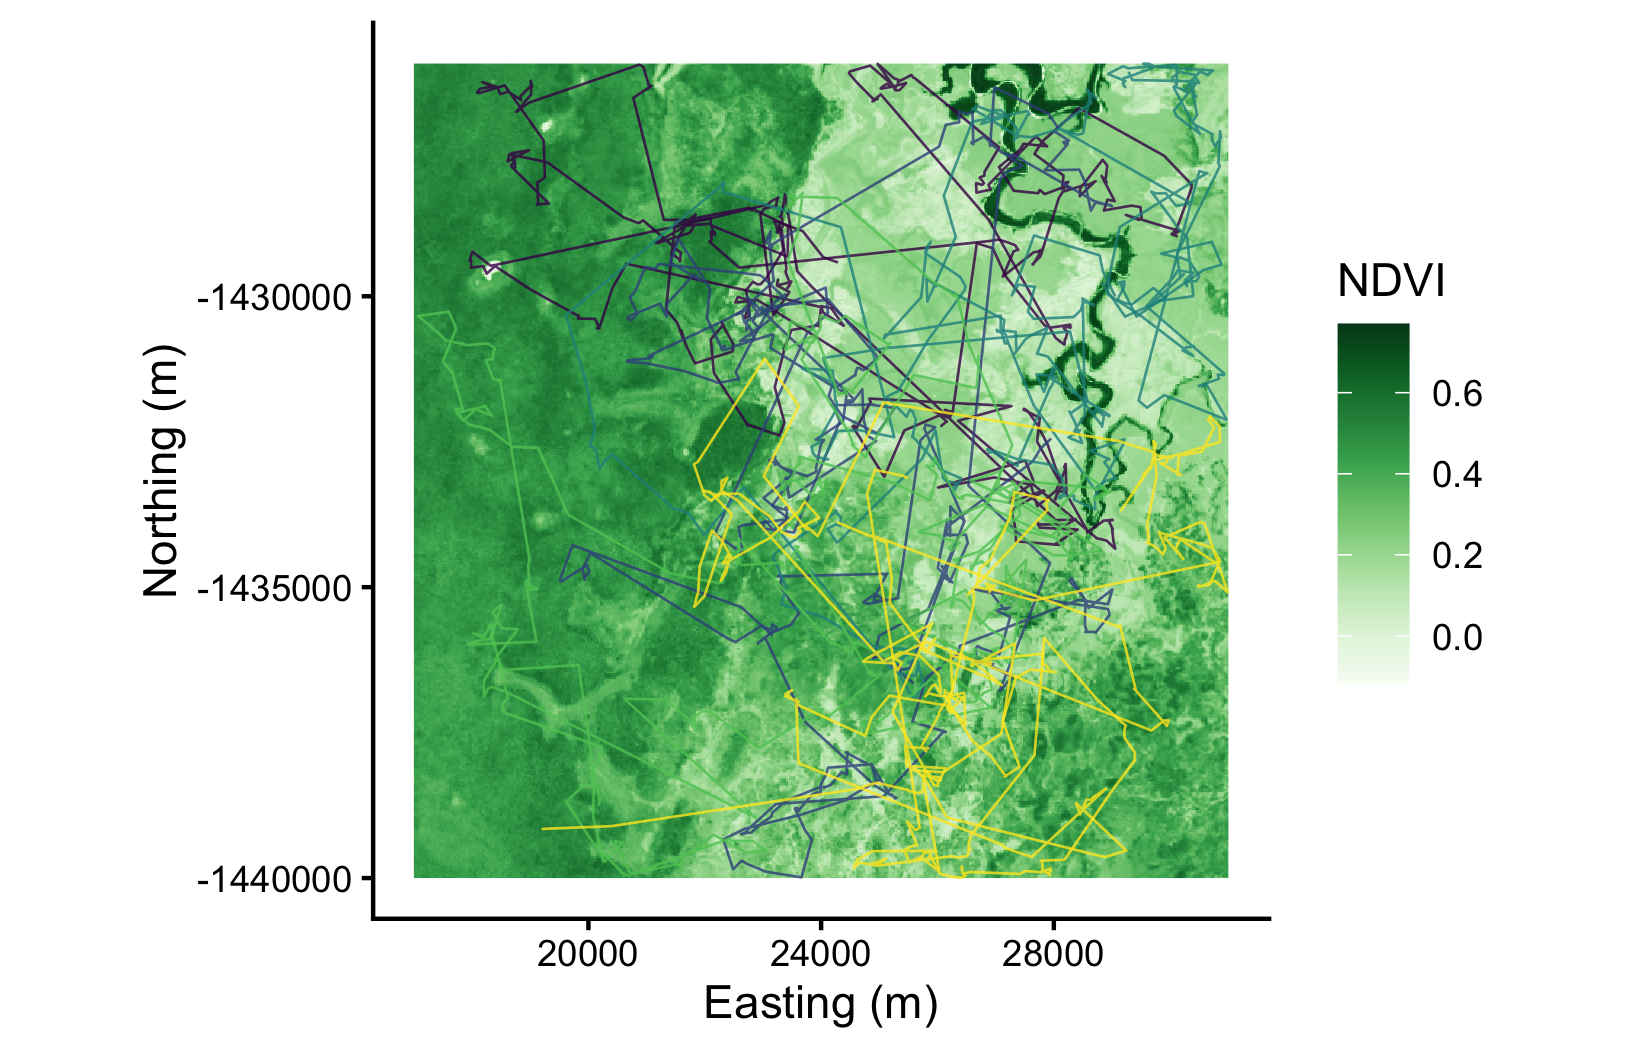
\includegraphics[keepaspectratio]{predictive_SSF_walkthrough_files/figure-pdf/example_trajectories-1.png}}

}

\caption{Five example simulated trajectories from the dynamic model,
over the NDVI layer.}

\end{figure}%

\begin{Shaded}
\begin{Highlighting}[]
\FunctionTok{bind\_rows}\NormalTok{(}
\NormalTok{  sims\_static  }\SpecialCharTok{\%\textgreater{}\%} \FunctionTok{select}\NormalTok{(hour, sl, model),}
\NormalTok{  sims\_dynamic }\SpecialCharTok{\%\textgreater{}\%} \FunctionTok{select}\NormalTok{(hour, sl, model)}
\NormalTok{) }\SpecialCharTok{\%\textgreater{}\%}
  \FunctionTok{group\_by}\NormalTok{(model, hour) }\SpecialCharTok{\%\textgreater{}\%}
  \FunctionTok{summarise}\NormalTok{(}\AttributeTok{mean\_sl =} \FunctionTok{mean}\NormalTok{(sl, }\AttributeTok{na.rm =} \ConstantTok{TRUE}\NormalTok{), }\AttributeTok{.groups =} \StringTok{"drop"}\NormalTok{) }\SpecialCharTok{\%\textgreater{}\%}
  \FunctionTok{bind\_rows}\NormalTok{(}
\NormalTok{    buffalo\_steps }\SpecialCharTok{\%\textgreater{}\%}
      \FunctionTok{mutate}\NormalTok{(}\AttributeTok{hour =} \FunctionTok{hour}\NormalTok{(t1\_)) }\SpecialCharTok{\%\textgreater{}\%}
      \FunctionTok{group\_by}\NormalTok{(hour) }\SpecialCharTok{\%\textgreater{}\%}
      \FunctionTok{summarise}\NormalTok{(}\AttributeTok{mean\_sl =} \FunctionTok{mean}\NormalTok{(sl\_, }\AttributeTok{na.rm =} \ConstantTok{TRUE}\NormalTok{), }\AttributeTok{.groups =} \StringTok{"drop"}\NormalTok{) }\SpecialCharTok{\%\textgreater{}\%}
      \FunctionTok{mutate}\NormalTok{(}\AttributeTok{model =} \StringTok{"Observed"}\NormalTok{)}
\NormalTok{  ) }\SpecialCharTok{\%\textgreater{}\%}
  \FunctionTok{ggplot}\NormalTok{(}\FunctionTok{aes}\NormalTok{(}\AttributeTok{x =}\NormalTok{ hour, }\AttributeTok{y =}\NormalTok{ mean\_sl, }\AttributeTok{colour =}\NormalTok{ model)) }\SpecialCharTok{+}
  \FunctionTok{geom\_line}\NormalTok{(}\AttributeTok{linewidth =} \FloatTok{0.9}\NormalTok{) }\SpecialCharTok{+}
  \FunctionTok{scale\_colour\_manual}\NormalTok{(}\AttributeTok{values =} \FunctionTok{c}\NormalTok{(}\StringTok{"A: static"} \OtherTok{=} \StringTok{"grey40"}\NormalTok{,}
                                 \StringTok{"B: temporally dynamic"} \OtherTok{=} \StringTok{"steelblue"}\NormalTok{,}
                                 \StringTok{"Observed"} \OtherTok{=} \StringTok{"red"}\NormalTok{), }\AttributeTok{name =} \ConstantTok{NULL}\NormalTok{) }\SpecialCharTok{+}
  \FunctionTok{scale\_x\_continuous}\NormalTok{(}\StringTok{"Hour of day"}\NormalTok{, }\AttributeTok{breaks =} \FunctionTok{seq}\NormalTok{(}\DecValTok{0}\NormalTok{, }\DecValTok{24}\NormalTok{, }\DecValTok{6}\NormalTok{)) }\SpecialCharTok{+}
  \FunctionTok{labs}\NormalTok{(}\AttributeTok{y =} \StringTok{"Mean step length (m)"}\NormalTok{) }\SpecialCharTok{+}
  \FunctionTok{theme\_classic}\NormalTok{() }\SpecialCharTok{+}
  \FunctionTok{theme}\NormalTok{(}\AttributeTok{legend.position =} \StringTok{"bottom"}\NormalTok{)}
\end{Highlighting}
\end{Shaded}

\begin{figure}[H]

{\centering \pandocbounded{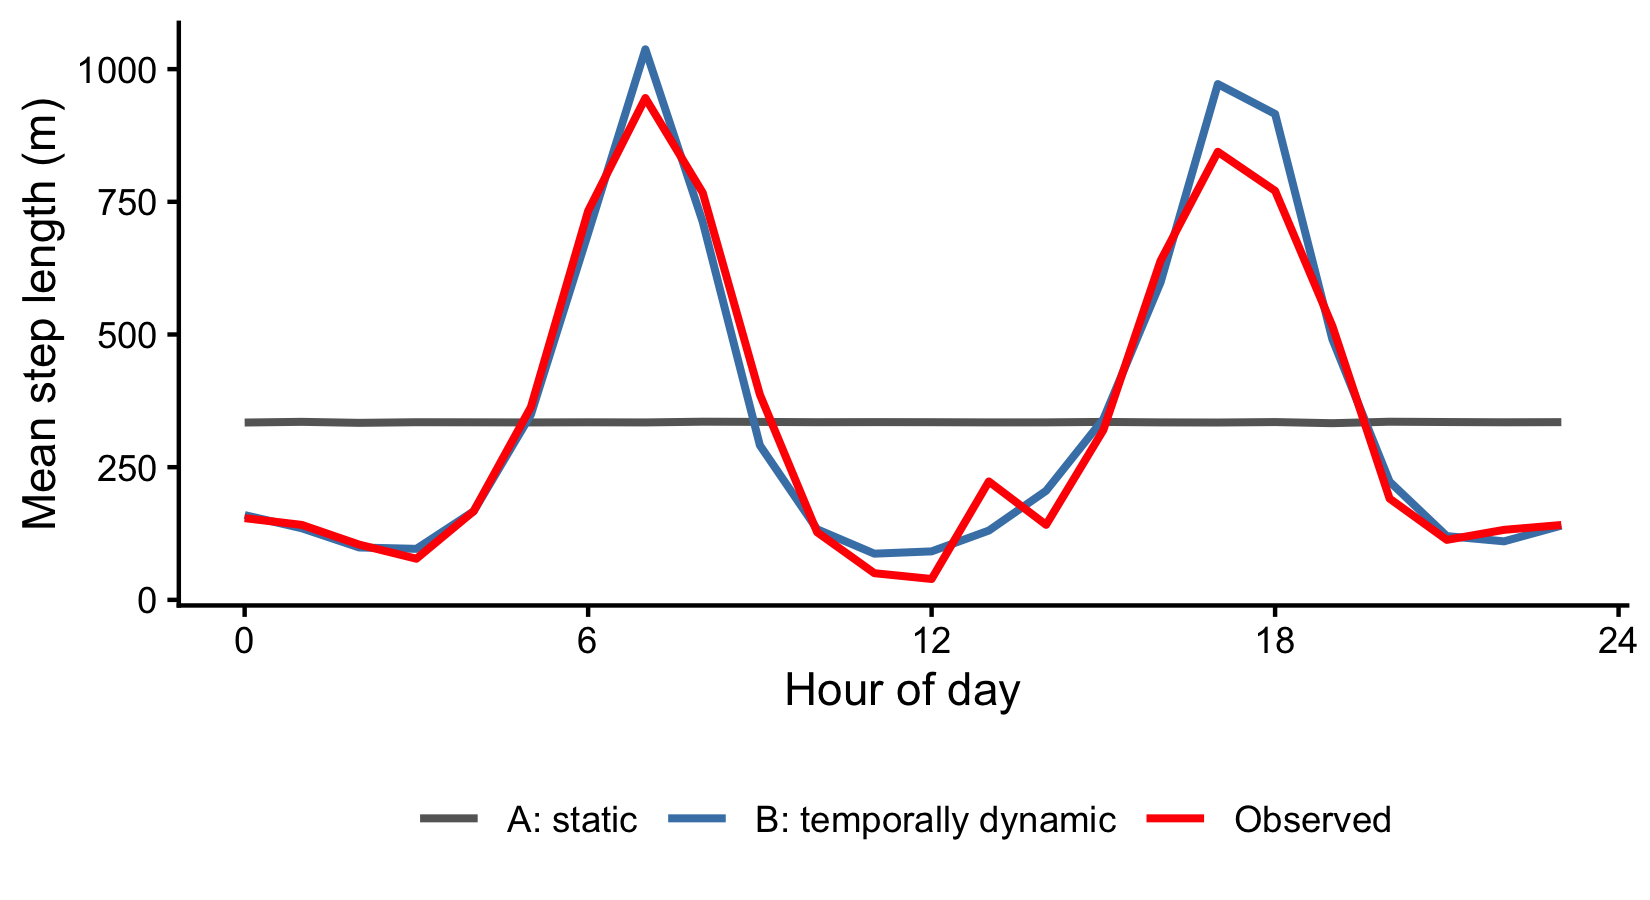
\includegraphics[keepaspectratio]{predictive_SSF_walkthrough_files/figure-pdf/plot_simulated_step_lengths-1.png}}

}

\caption{Hourly mean step length in the simulations, compared with the
observed data.}

\end{figure}%

An immediate and encouraging result: the dynamic model reproduces the
observed daily activity cycle closely, while the static model --- which
cannot do otherwise --- predicts a flat line.

\section{9. Aggregating simulations into utilisation
distributions}\label{aggregating-simulations-into-utilisation-distributions}

A single simulated trajectory is one realisation of a stochastic process
and tells us little. The prediction is in the \emph{ensemble}: count how
often simulated animals occupy each cell of the landscape, and the
result is a predicted utilisation distribution (UD).

\begin{Shaded}
\begin{Highlighting}[]
\CommentTok{\#\textquotesingle{} Aggregate simulated locations into a normalised utilisation distribution}
\CommentTok{\#\textquotesingle{}}
\CommentTok{\#\textquotesingle{} @param sims       data frame of simulated locations}
\CommentTok{\#\textquotesingle{} @param resolution cell size in metres}
\CommentTok{\#\textquotesingle{} @param hours      optionally restrict to particular hours of the day}
\NormalTok{aggregate\_to\_ud }\OtherTok{\textless{}{-}} \ControlFlowTok{function}\NormalTok{(sims, resolution, }\AttributeTok{hours =} \ConstantTok{NULL}\NormalTok{) \{}

  \ControlFlowTok{if}\NormalTok{ (}\SpecialCharTok{!}\FunctionTok{is.null}\NormalTok{(hours)) sims }\OtherTok{\textless{}{-}}\NormalTok{ sims }\SpecialCharTok{\%\textgreater{}\%} \FunctionTok{filter}\NormalTok{(hour }\SpecialCharTok{\%in\%}\NormalTok{ hours)}

\NormalTok{  template }\OtherTok{\textless{}{-}} \FunctionTok{rast}\NormalTok{(}\AttributeTok{extent =} \FunctionTok{ext}\NormalTok{(ndvi\_crop), }\AttributeTok{resolution =}\NormalTok{ resolution,}
                   \AttributeTok{crs =} \FunctionTok{crs}\NormalTok{(ndvi\_crop))}

  \CommentTok{\# Count the simulated locations falling in each cell}
\NormalTok{  counts }\OtherTok{\textless{}{-}}\NormalTok{ terra}\SpecialCharTok{::}\FunctionTok{rasterize}\NormalTok{(}\FunctionTok{cbind}\NormalTok{(sims}\SpecialCharTok{$}\NormalTok{x, sims}\SpecialCharTok{$}\NormalTok{y), template, }\AttributeTok{fun =} \StringTok{"sum"}\NormalTok{)}

  \CommentTok{\# Cells with no simulated locations are true zeroes, not missing data}
\NormalTok{  counts[}\FunctionTok{is.na}\NormalTok{(counts)] }\OtherTok{\textless{}{-}} \DecValTok{0}

  \CommentTok{\# Normalise so that the layer sums to 1, making models comparable}
\NormalTok{  counts }\SpecialCharTok{/} \FunctionTok{global}\NormalTok{(counts, }\StringTok{"sum"}\NormalTok{, }\AttributeTok{na.rm =} \ConstantTok{TRUE}\NormalTok{)[[}\DecValTok{1}\NormalTok{]]}
\NormalTok{\}}
\end{Highlighting}
\end{Shaded}

\begin{Shaded}
\begin{Highlighting}[]
\FunctionTok{tic}\NormalTok{(}\StringTok{"Aggregating simulations"}\NormalTok{)}
\NormalTok{ud\_static      }\OtherTok{\textless{}{-}} \FunctionTok{aggregate\_to\_ud}\NormalTok{(sims\_static,      ud\_res)}
\NormalTok{ud\_dynamic     }\OtherTok{\textless{}{-}} \FunctionTok{aggregate\_to\_ud}\NormalTok{(sims\_dynamic,     ud\_res)}
\NormalTok{ud\_dynamic\_obs }\OtherTok{\textless{}{-}} \FunctionTok{aggregate\_to\_ud}\NormalTok{(sims\_dynamic\_obs, ud\_res)}
\FunctionTok{toc}\NormalTok{()}
\end{Highlighting}
\end{Shaded}

\begin{verbatim}
Aggregating simulations: 1.148 sec elapsed
\end{verbatim}

\begin{Shaded}
\begin{Highlighting}[]
\CommentTok{\# Check that each normalises to 1}
\FunctionTok{cat}\NormalTok{(}\StringTok{"Sum of UD values {-} static:"}\NormalTok{,}
    \FunctionTok{round}\NormalTok{(}\FunctionTok{global}\NormalTok{(ud\_static, }\StringTok{"sum"}\NormalTok{, }\AttributeTok{na.rm =} \ConstantTok{TRUE}\NormalTok{)[[}\DecValTok{1}\NormalTok{]], }\DecValTok{6}\NormalTok{),}
    \StringTok{" dynamic:"}\NormalTok{,}
    \FunctionTok{round}\NormalTok{(}\FunctionTok{global}\NormalTok{(ud\_dynamic, }\StringTok{"sum"}\NormalTok{, }\AttributeTok{na.rm =} \ConstantTok{TRUE}\NormalTok{)[[}\DecValTok{1}\NormalTok{]], }\DecValTok{6}\NormalTok{), }\StringTok{"}\SpecialCharTok{\textbackslash{}n}\StringTok{"}\NormalTok{)}
\end{Highlighting}
\end{Shaded}

\begin{verbatim}
Sum of UD values - static: 1  dynamic: 1 
\end{verbatim}

\begin{Shaded}
\begin{Highlighting}[]
\NormalTok{plot\_ud }\OtherTok{\textless{}{-}} \ControlFlowTok{function}\NormalTok{(ud, title) \{}
\NormalTok{  df }\OtherTok{\textless{}{-}} \FunctionTok{as.data.frame}\NormalTok{(ud, }\AttributeTok{xy =} \ConstantTok{TRUE}\NormalTok{)}
  \FunctionTok{names}\NormalTok{(df)[}\DecValTok{3}\NormalTok{] }\OtherTok{\textless{}{-}} \StringTok{"density"}

  \FunctionTok{ggplot}\NormalTok{() }\SpecialCharTok{+}
    \FunctionTok{geom\_raster}\NormalTok{(}\AttributeTok{data =}\NormalTok{ df, }\FunctionTok{aes}\NormalTok{(}\AttributeTok{x =}\NormalTok{ x, }\AttributeTok{y =}\NormalTok{ y, }\AttributeTok{fill =} \FunctionTok{log10}\NormalTok{(density }\SpecialCharTok{+} \FloatTok{1e{-}8}\NormalTok{))) }\SpecialCharTok{+}
    \FunctionTok{geom\_point}\NormalTok{(}\AttributeTok{data =}\NormalTok{ buffalo\_id, }\FunctionTok{aes}\NormalTok{(}\AttributeTok{x =}\NormalTok{ x\_, }\AttributeTok{y =}\NormalTok{ y\_),}
               \AttributeTok{colour =} \StringTok{"red"}\NormalTok{, }\AttributeTok{size =} \FloatTok{0.15}\NormalTok{, }\AttributeTok{alpha =} \FloatTok{0.15}\NormalTok{) }\SpecialCharTok{+}
    \FunctionTok{scale\_fill\_viridis\_c}\NormalTok{(}\StringTok{"log10}\SpecialCharTok{\textbackslash{}n}\StringTok{density"}\NormalTok{, }\AttributeTok{option =} \StringTok{"magma"}\NormalTok{) }\SpecialCharTok{+}
    \FunctionTok{coord\_equal}\NormalTok{() }\SpecialCharTok{+}
    \FunctionTok{labs}\NormalTok{(}\AttributeTok{title =}\NormalTok{ title, }\AttributeTok{x =} \ConstantTok{NULL}\NormalTok{, }\AttributeTok{y =} \ConstantTok{NULL}\NormalTok{) }\SpecialCharTok{+}
    \FunctionTok{theme\_classic}\NormalTok{() }\SpecialCharTok{+}
    \FunctionTok{theme}\NormalTok{(}\AttributeTok{axis.text =} \FunctionTok{element\_text}\NormalTok{(}\AttributeTok{size =} \DecValTok{6}\NormalTok{),}
          \AttributeTok{plot.title =} \FunctionTok{element\_text}\NormalTok{(}\AttributeTok{size =} \DecValTok{10}\NormalTok{))}
\NormalTok{\}}

\FunctionTok{plot\_ud}\NormalTok{(ud\_static, }\StringTok{"A: static"}\NormalTok{) }\SpecialCharTok{+} \FunctionTok{plot\_ud}\NormalTok{(ud\_dynamic, }\StringTok{"B: temporally dynamic"}\NormalTok{)}
\end{Highlighting}
\end{Shaded}

\begin{figure}[H]

{\centering \pandocbounded{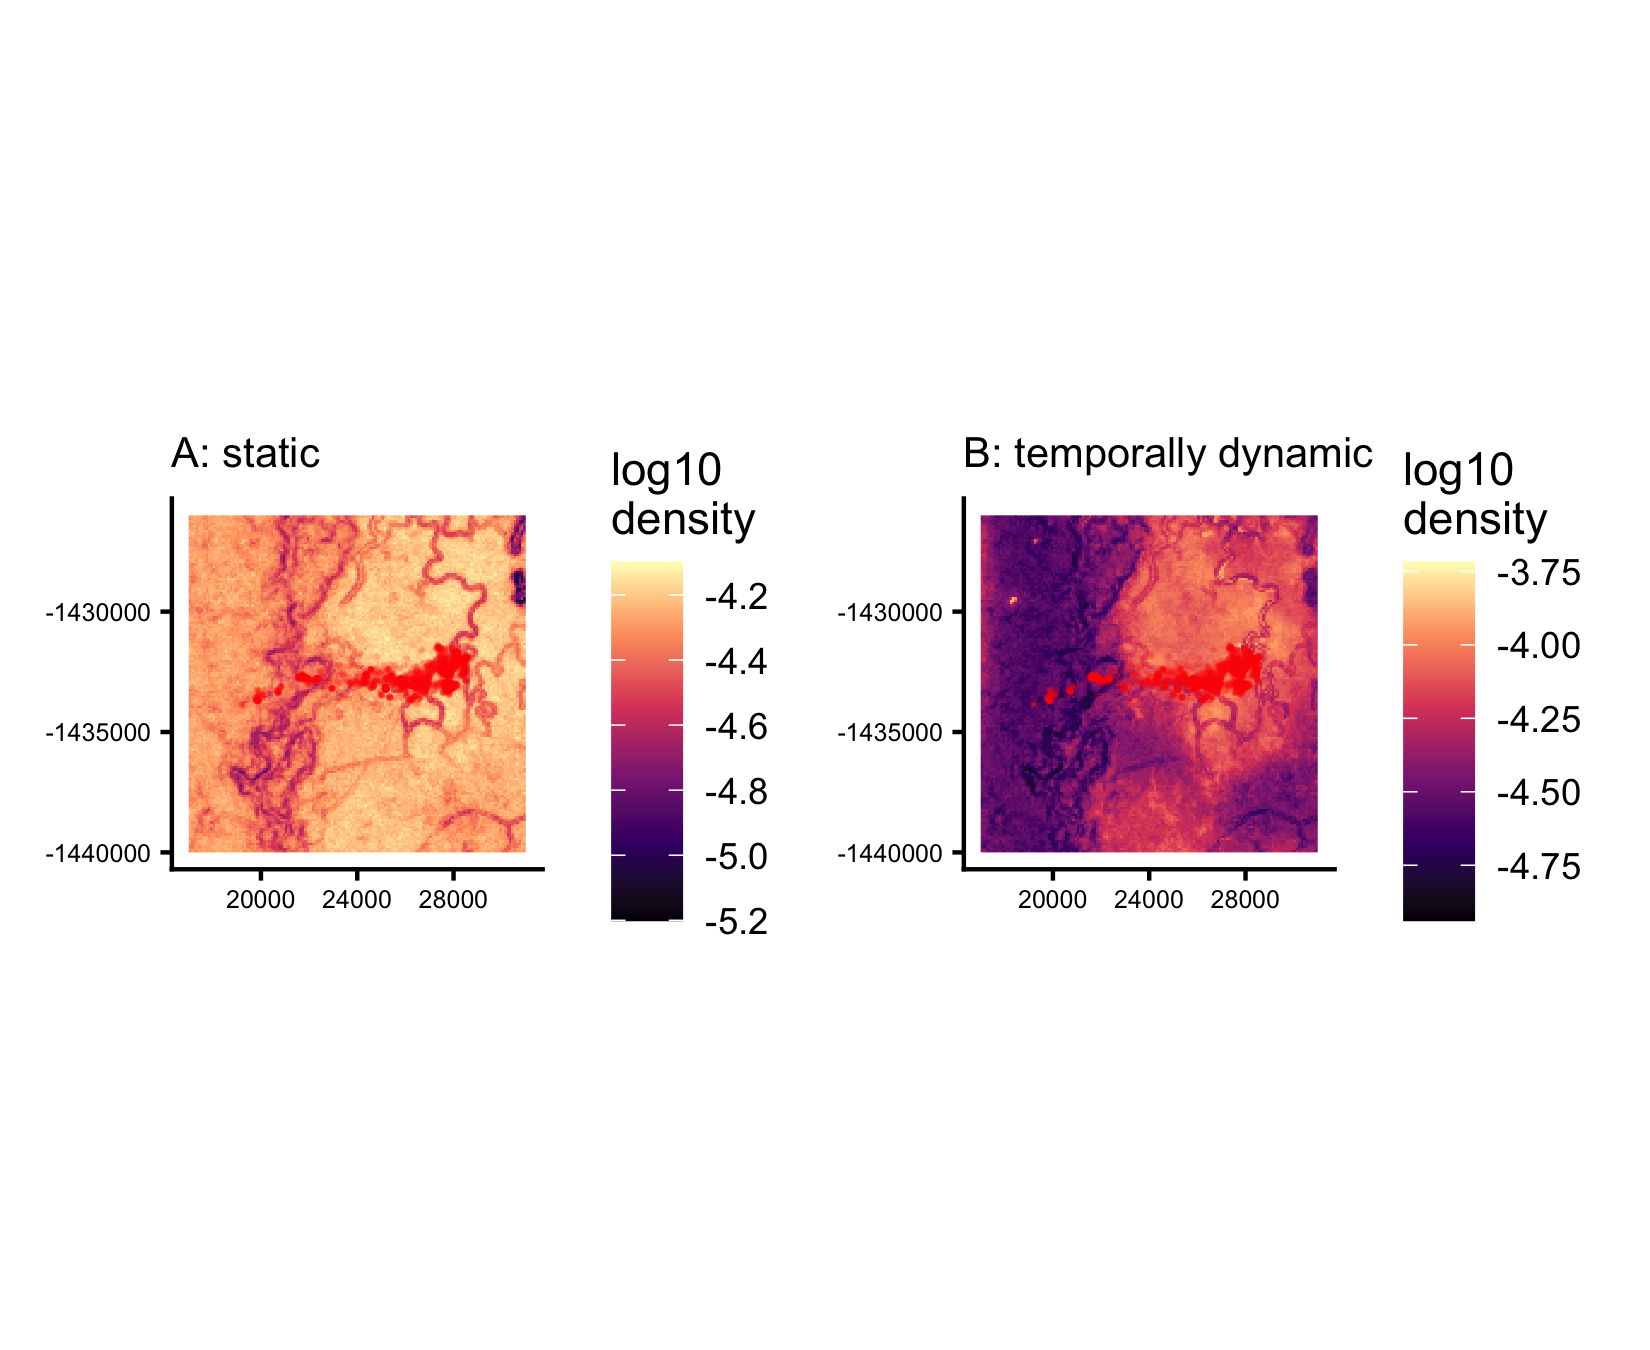
\includegraphics[keepaspectratio]{predictive_SSF_walkthrough_files/figure-pdf/plot_uds-1.png}}

}

\caption{Predicted utilisation distributions (log scale) with observed
locations in red.}

\end{figure}%

\subsection{The effect of the starting
location}\label{the-effect-of-the-starting-location}

\begin{Shaded}
\begin{Highlighting}[]
\FunctionTok{plot\_ud}\NormalTok{(ud\_dynamic, }\StringTok{"Random starts (stationary distribution)"}\NormalTok{) }\SpecialCharTok{+}
  \FunctionTok{plot\_ud}\NormalTok{(ud\_dynamic\_obs, }\StringTok{"Observed start (home{-}range{-}like)"}\NormalTok{)}
\end{Highlighting}
\end{Shaded}

\begin{figure}[H]

{\centering \pandocbounded{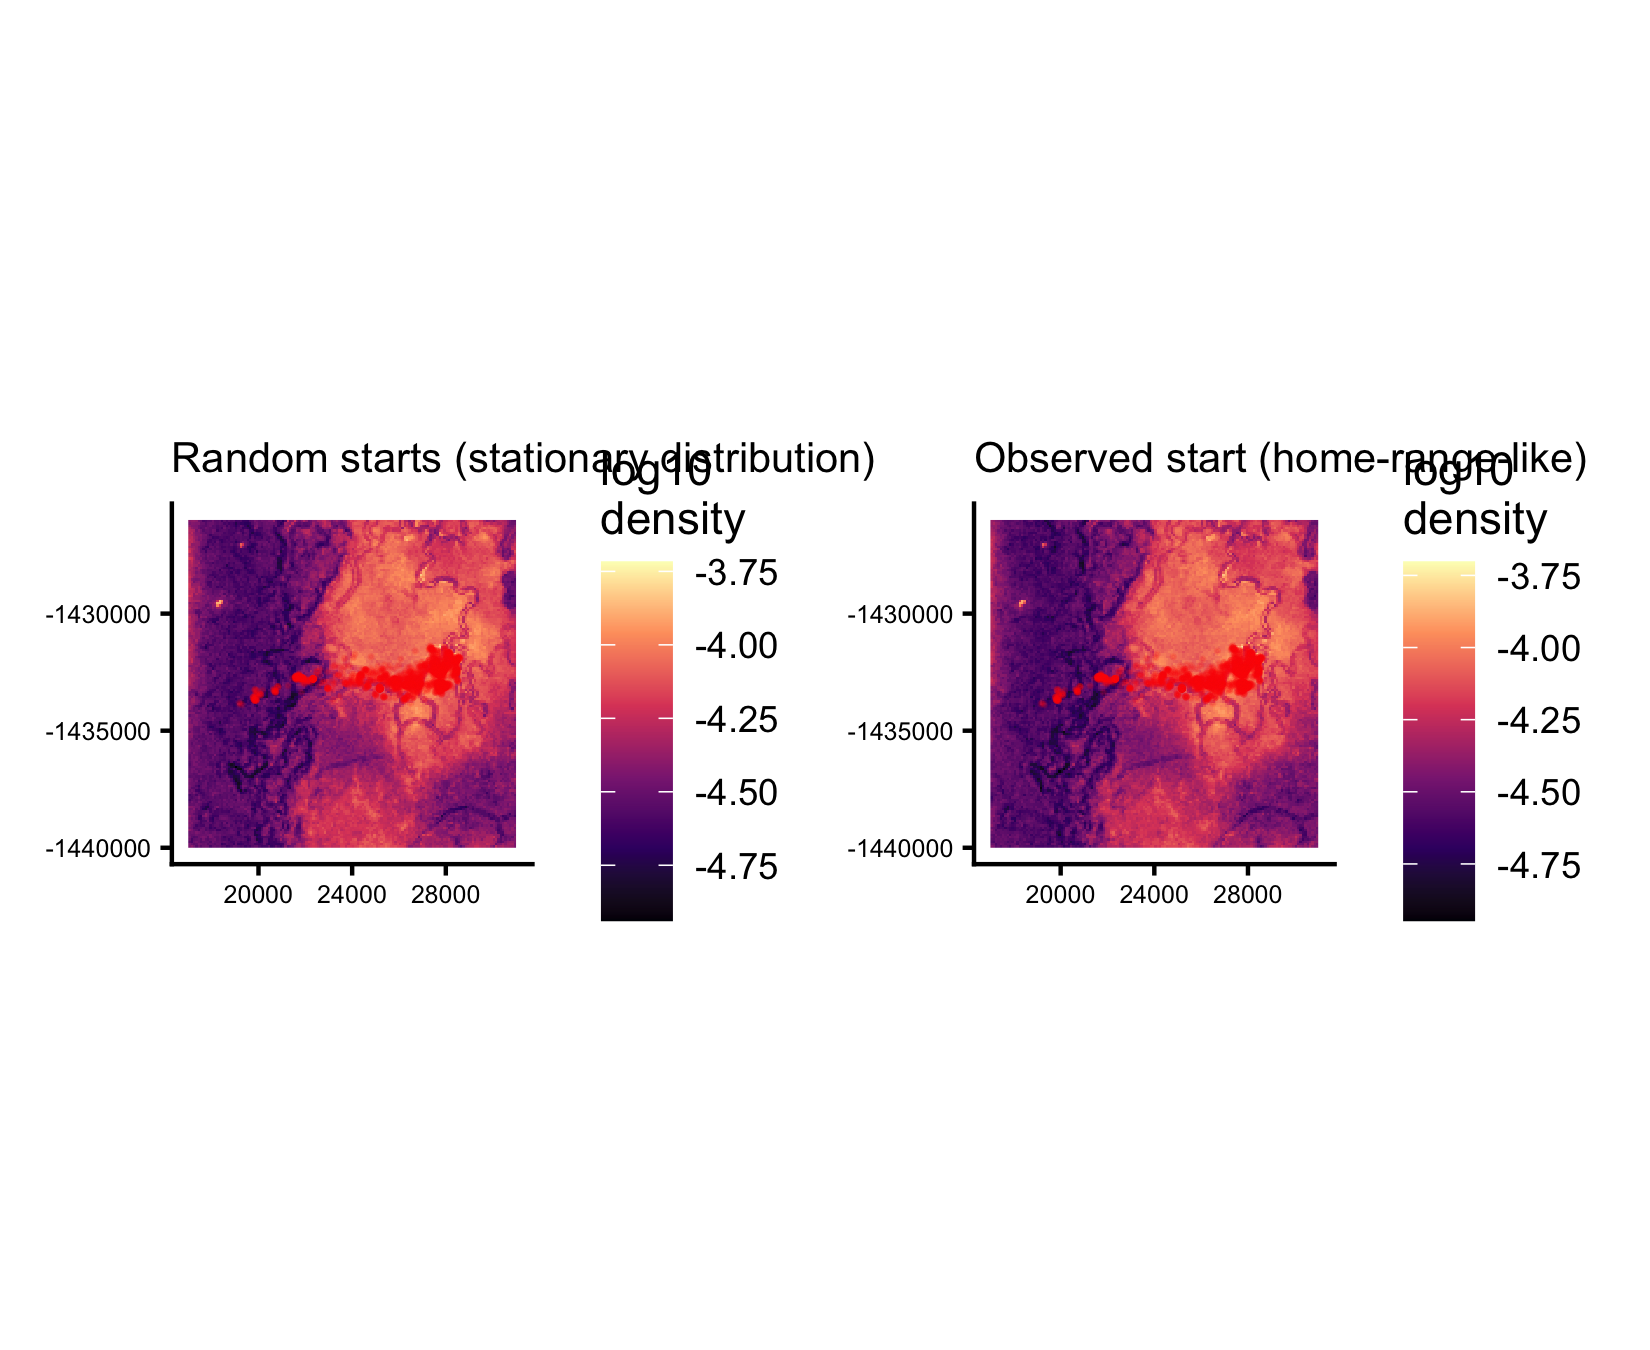
\includegraphics[keepaspectratio]{predictive_SSF_walkthrough_files/figure-pdf/plot_start_comparison-1.png}}

}

\caption{The same model, seeded uniformly at random across the landscape
(left) and from the animal's observed starting location (right).}

\end{figure}%

Two quite different predictions, from the same fitted model. Seeded at
random, the simulation describes where an animal following this movement
process would be found \emph{anywhere} in this landscape over the long
run. Seeded from the observed start, it describes where \emph{this}
animal was likely to range over the following 30 days. Neither is more
correct; they answer different questions, and it is worth being explicit
about which one is being asked.

\subsection{Has the simulation
converged?}\label{has-the-simulation-converged}

How many trajectories are enough? We can answer empirically, and
cheaply, by reusing the trajectories we already have: build UDs from
increasing subsets and see how quickly they stabilise towards the full
result.

\begin{Shaded}
\begin{Highlighting}[]
\NormalTok{subset\_sizes }\OtherTok{\textless{}{-}} \FunctionTok{c}\NormalTok{(}\DecValTok{10}\NormalTok{, }\DecValTok{25}\NormalTok{, }\DecValTok{50}\NormalTok{, }\DecValTok{100}\NormalTok{, }\DecValTok{250}\NormalTok{, }\DecValTok{1000}\NormalTok{, }\DecValTok{5000}\NormalTok{, n\_traj)}

\CommentTok{\# Run the check at two aggregation resolutions, because the number of}
\CommentTok{\# trajectories needed depends on how finely we are asking the question}
\NormalTok{convergence }\OtherTok{\textless{}{-}} \FunctionTok{map\_dfr}\NormalTok{(}\FunctionTok{c}\NormalTok{(ud\_res, ud\_res\_hourly), }\ControlFlowTok{function}\NormalTok{(resolution) \{}
\NormalTok{  ud\_full }\OtherTok{\textless{}{-}} \FunctionTok{aggregate\_to\_ud}\NormalTok{(sims\_dynamic, resolution)}
  \FunctionTok{map\_dfr}\NormalTok{(subset\_sizes, }\ControlFlowTok{function}\NormalTok{(n) \{}
\NormalTok{    ud\_n }\OtherTok{\textless{}{-}} \FunctionTok{aggregate\_to\_ud}\NormalTok{(sims\_dynamic }\SpecialCharTok{\%\textgreater{}\%} \FunctionTok{filter}\NormalTok{(traj\_id }\SpecialCharTok{\textless{}=}\NormalTok{ n), resolution)}
    \FunctionTok{data.frame}\NormalTok{(}
      \AttributeTok{resolution =} \FunctionTok{paste0}\NormalTok{(resolution, }\StringTok{" m"}\NormalTok{),}
      \AttributeTok{n\_trajectories =}\NormalTok{ n,}
      \AttributeTok{correlation =} \FunctionTok{cor}\NormalTok{(}\FunctionTok{values}\NormalTok{(ud\_n)[, }\DecValTok{1}\NormalTok{], }\FunctionTok{values}\NormalTok{(ud\_full)[, }\DecValTok{1}\NormalTok{],}
                        \AttributeTok{use =} \StringTok{"complete.obs"}\NormalTok{, }\AttributeTok{method =} \StringTok{"spearman"}\NormalTok{)}
\NormalTok{    )}
\NormalTok{  \})}
\NormalTok{\})}

\FunctionTok{ggplot}\NormalTok{(convergence, }\FunctionTok{aes}\NormalTok{(}\AttributeTok{x =}\NormalTok{ n\_trajectories, }\AttributeTok{y =}\NormalTok{ correlation, }\AttributeTok{colour =}\NormalTok{ resolution)) }\SpecialCharTok{+}
  \FunctionTok{geom\_line}\NormalTok{(}\AttributeTok{linewidth =} \FloatTok{0.9}\NormalTok{) }\SpecialCharTok{+}
  \FunctionTok{geom\_point}\NormalTok{(}\AttributeTok{size =} \DecValTok{2}\NormalTok{) }\SpecialCharTok{+}
  \FunctionTok{scale\_x\_log10}\NormalTok{(}\StringTok{"Number of trajectories"}\NormalTok{) }\SpecialCharTok{+}
  \FunctionTok{scale\_y\_continuous}\NormalTok{(}\StringTok{"Spearman correlation with full UD"}\NormalTok{, }\AttributeTok{limits =} \FunctionTok{c}\NormalTok{(}\DecValTok{0}\NormalTok{, }\DecValTok{1}\NormalTok{)) }\SpecialCharTok{+}
  \FunctionTok{scale\_colour\_manual}\NormalTok{(}\AttributeTok{values =} \FunctionTok{c}\NormalTok{(}\StringTok{"steelblue"}\NormalTok{, }\StringTok{"darkorange"}\NormalTok{), }\AttributeTok{name =} \StringTok{"Aggregation"}\NormalTok{) }\SpecialCharTok{+}
  \FunctionTok{theme\_classic}\NormalTok{() }\SpecialCharTok{+}
  \FunctionTok{theme}\NormalTok{(}\AttributeTok{legend.position =} \StringTok{"bottom"}\NormalTok{)}
\end{Highlighting}
\end{Shaded}

\begin{figure}[H]

{\centering \pandocbounded{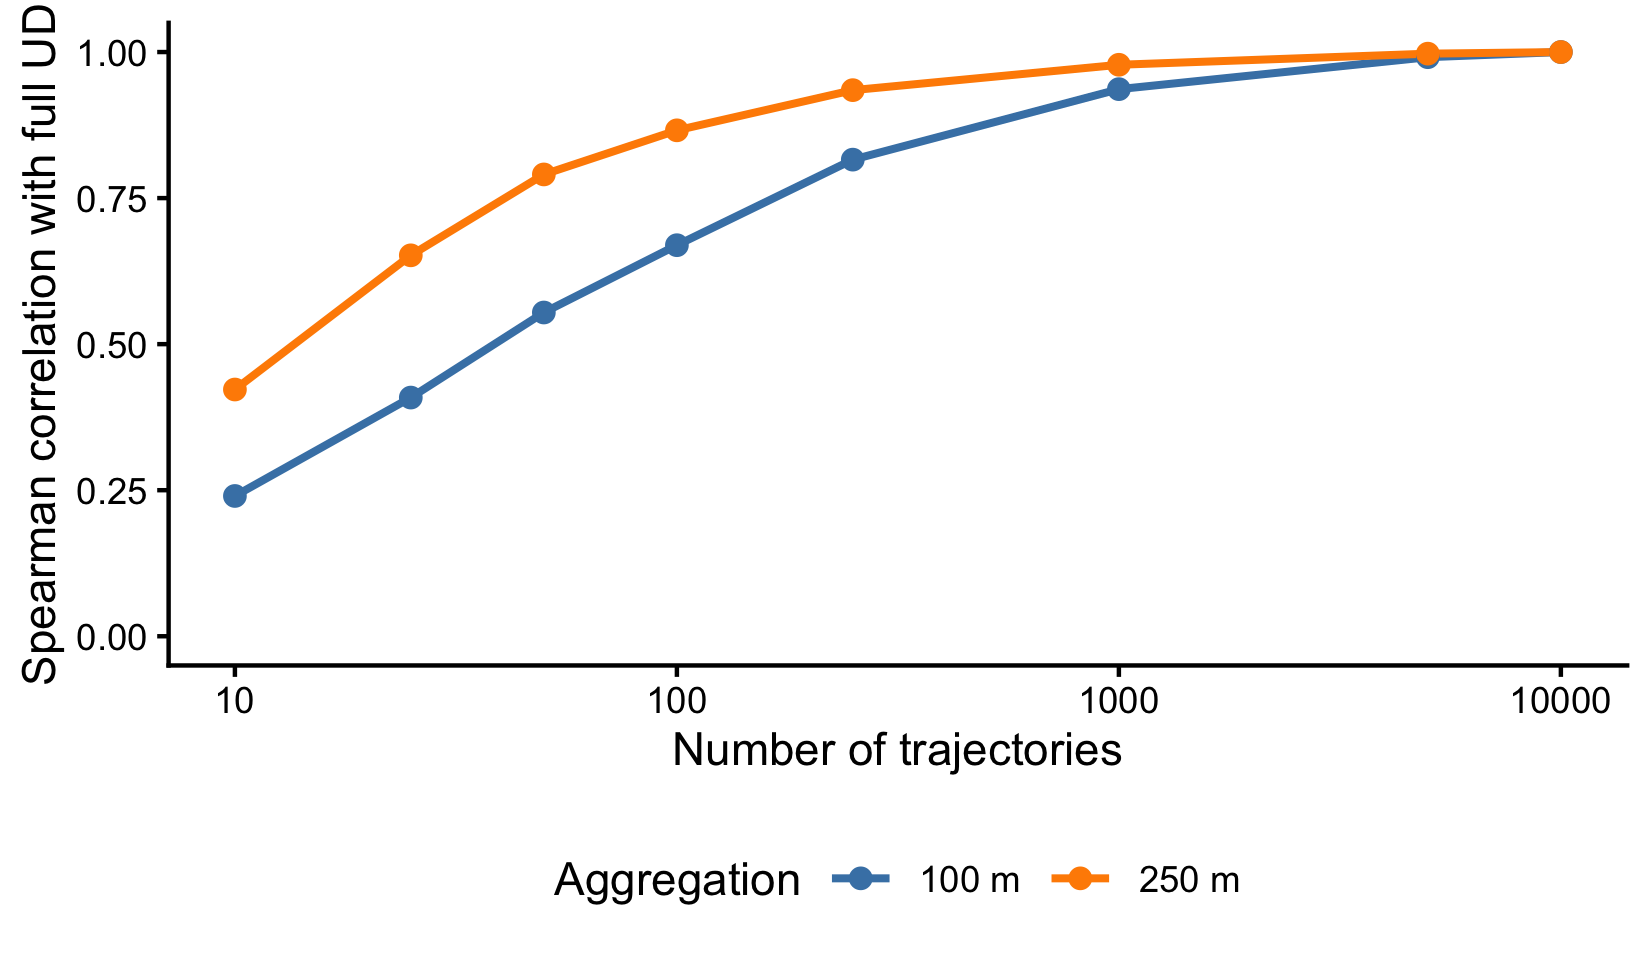
\includegraphics[keepaspectratio]{predictive_SSF_walkthrough_files/figure-pdf/convergence-1.png}}

}

\caption{Correlation between a UD built from n trajectories and the UD
built from all of them.}

\end{figure}%

\begin{Shaded}
\begin{Highlighting}[]
\NormalTok{convergence }\SpecialCharTok{\%\textgreater{}\%} \FunctionTok{pivot\_wider}\NormalTok{(}\AttributeTok{names\_from =}\NormalTok{ resolution, }\AttributeTok{values\_from =}\NormalTok{ correlation)}
\end{Highlighting}
\end{Shaded}

\begin{verbatim}
# A tibble: 7 x 3
  n_trajectories `100 m`   `250 m`  
           <dbl> <list>    <list>   
1             10 <dbl [1]> <dbl [1]>
2             25 <dbl [1]> <dbl [1]>
3             50 <dbl [1]> <dbl [1]>
4            100 <dbl [1]> <dbl [1]>
5            250 <dbl [1]> <dbl [1]>
6           1000 <dbl [2]> <dbl [2]>
7           5000 <dbl [1]> <dbl [1]>
\end{verbatim}

\begin{tcolorbox}[enhanced jigsaw, arc=.35mm, bottomrule=.15mm, bottomtitle=1mm, breakable, colback=white, colbacktitle=quarto-callout-important-color!10!white, colframe=quarto-callout-important-color-frame, coltitle=black, left=2mm, leftrule=.75mm, opacityback=0, opacitybacktitle=0.6, rightrule=.15mm, title=\textcolor{quarto-callout-important-color}{\faExclamation}\hspace{0.5em}{This simulation has \emph{not} converged}, titlerule=0mm, toprule=.15mm, toptitle=1mm]

At the 100 m aggregation the curve is still climbing steeply at 250
trajectories --- it has not levelled off, which means 1000 trajectories
is \textbf{not} enough to characterise the utilisation distribution at
that resolution. With 1,416,000 simulated locations spread over a 100 m
grid, most cells hold only a handful of points, so the map is still
substantially sampling noise.

This is worth showing rather than quietly fixing, because it is the
check itself that is the lesson: had we simply looked at the map, it
would have appeared perfectly plausible. Two levers are available, and
the second curve shows the second of them:

\begin{itemize}
\tightlist
\item
  \textbf{More trajectories.} Forrest et al. (2025) used 100,000
  trajectories of 3,000 steps, run on a computing cluster. Increase
  \texttt{n\_traj} in the parameter block.
\item
  \textbf{Coarser aggregation.} The same simulations converge much
  faster at 250 m, because each cell collects more points. If the
  ecological question does not require 100 m resolution, this is free.
\end{itemize}

Note also that this is a \emph{self-consistency} check --- it asks
whether the answer has stopped changing, not whether it is right. A
converged UD can still be a converged estimate of a bad model.

\end{tcolorbox}

The results below should therefore be read as an illustration of the
method rather than as a definitive statement about this animal.

\subsection{Hourly utilisation
distributions}\label{hourly-utilisation-distributions}

The dynamic model's real claim is not just about where the animal goes,
but about \emph{when}. We therefore also aggregate separately for each
hour of the day.

\begin{Shaded}
\begin{Highlighting}[]
\FunctionTok{tic}\NormalTok{(}\StringTok{"Building hourly UDs"}\NormalTok{)}
\NormalTok{uds\_hourly\_static  }\OtherTok{\textless{}{-}} \FunctionTok{rast}\NormalTok{(}\FunctionTok{map}\NormalTok{(}\DecValTok{0}\SpecialCharTok{:}\DecValTok{23}\NormalTok{, }\SpecialCharTok{\textasciitilde{}} \FunctionTok{aggregate\_to\_ud}\NormalTok{(sims\_static,  ud\_res\_hourly, }\AttributeTok{hours =}\NormalTok{ .x)))}
\NormalTok{uds\_hourly\_dynamic }\OtherTok{\textless{}{-}} \FunctionTok{rast}\NormalTok{(}\FunctionTok{map}\NormalTok{(}\DecValTok{0}\SpecialCharTok{:}\DecValTok{23}\NormalTok{, }\SpecialCharTok{\textasciitilde{}} \FunctionTok{aggregate\_to\_ud}\NormalTok{(sims\_dynamic, ud\_res\_hourly, }\AttributeTok{hours =}\NormalTok{ .x)))}
\FunctionTok{toc}\NormalTok{()}
\end{Highlighting}
\end{Shaded}

\begin{verbatim}
Building hourly UDs: 1.744 sec elapsed
\end{verbatim}

\begin{Shaded}
\begin{Highlighting}[]
\FunctionTok{names}\NormalTok{(uds\_hourly\_static)  }\OtherTok{\textless{}{-}} \FunctionTok{paste0}\NormalTok{(}\StringTok{"hour\_"}\NormalTok{, }\DecValTok{0}\SpecialCharTok{:}\DecValTok{23}\NormalTok{)}
\FunctionTok{names}\NormalTok{(uds\_hourly\_dynamic) }\OtherTok{\textless{}{-}} \FunctionTok{paste0}\NormalTok{(}\StringTok{"hour\_"}\NormalTok{, }\DecValTok{0}\SpecialCharTok{:}\DecValTok{23}\NormalTok{)}

\NormalTok{uds\_hourly\_dynamic}
\end{Highlighting}
\end{Shaded}

\begin{verbatim}
class       : SpatRaster
size        : 56, 56, 24  (nrow, ncol, nlyr)
resolution  : 250, 250  (x, y)
extent      : 17000, 31000, -1440000, -1426000  (xmin, xmax, ymin, ymax)
coord. ref. : GDA94 / Geoscience Australia Lambert (EPSG:3112)
source(s)   : memory
names       :   hour_0,   hour_1,   hour_2,   hour_3,   hour_4,   hour_5, ...
min values  : 0.000017, 0.000017, 0.000017, 0.000017, 0.000017,        0, ...
max values  : 0.001085, 0.001102, 0.001119, 0.001051, 0.001153, 0.001237, ...
\end{verbatim}

\begin{Shaded}
\begin{Highlighting}[]
\NormalTok{ud\_gif\_path }\OtherTok{\textless{}{-}} \FunctionTok{file.path}\NormalTok{(plot\_save\_path, }\StringTok{"hourly\_uds.gif"}\NormalTok{)}

\CommentTok{\# A shared colour scale across all frames, on the log scale}
\NormalTok{hourly\_vals }\OtherTok{\textless{}{-}} \FunctionTok{values}\NormalTok{(uds\_hourly\_dynamic)}
\NormalTok{ud\_limits }\OtherTok{\textless{}{-}} \FunctionTok{range}\NormalTok{(}\FunctionTok{log10}\NormalTok{(hourly\_vals[hourly\_vals }\SpecialCharTok{\textgreater{}} \DecValTok{0}\NormalTok{]), }\AttributeTok{na.rm =} \ConstantTok{TRUE}\NormalTok{)}

\NormalTok{ud\_frames }\OtherTok{\textless{}{-}} \FunctionTok{map\_chr}\NormalTok{(}\DecValTok{0}\SpecialCharTok{:}\DecValTok{23}\NormalTok{, }\ControlFlowTok{function}\NormalTok{(h) \{}
\NormalTok{  f }\OtherTok{\textless{}{-}} \FunctionTok{file.path}\NormalTok{(plot\_save\_path, }\FunctionTok{sprintf}\NormalTok{(}\StringTok{"ud\_frame\_\%02d.png"}\NormalTok{, h))}
  \FunctionTok{png}\NormalTok{(f, }\AttributeTok{width =} \DecValTok{110}\NormalTok{, }\AttributeTok{height =} \DecValTok{110}\NormalTok{, }\AttributeTok{units =} \StringTok{"mm"}\NormalTok{, }\AttributeTok{res =} \DecValTok{150}\NormalTok{)}
  \FunctionTok{plot}\NormalTok{(}\FunctionTok{log10}\NormalTok{(uds\_hourly\_dynamic[[h }\SpecialCharTok{+} \DecValTok{1}\NormalTok{]]),}
       \AttributeTok{main =} \FunctionTok{sprintf}\NormalTok{(}\StringTok{"Predicted use, \%02d:00"}\NormalTok{, h),}
       \AttributeTok{range =}\NormalTok{ ud\_limits, }\AttributeTok{col =} \FunctionTok{viridis}\NormalTok{(}\DecValTok{100}\NormalTok{, }\AttributeTok{option =} \StringTok{"magma"}\NormalTok{))}
  \FunctionTok{dev.off}\NormalTok{()}
\NormalTok{  f}
\NormalTok{\})}

\FunctionTok{image\_read}\NormalTok{(ud\_frames) }\SpecialCharTok{\%\textgreater{}\%}
  \FunctionTok{image\_animate}\NormalTok{(}\AttributeTok{fps =} \DecValTok{4}\NormalTok{) }\SpecialCharTok{\%\textgreater{}\%}
  \FunctionTok{image\_write}\NormalTok{(ud\_gif\_path)}

\FunctionTok{unlink}\NormalTok{(ud\_frames)}
\end{Highlighting}
\end{Shaded}

\begin{figure}[H]

{\centering \pandocbounded{\includegraphics[keepaspectratio]{outputs/walkthrough/hourly_uds.gif}}

}

\caption{Hourly predicted utilisation distributions from the temporally
dynamic model.}

\end{figure}%

This is the payoff of the whole exercise. Predicted use is not a fixed
map but a landscape that shifts through the day, as the simulated
animals move between the habitats they select at different times.

\section{10. Hourly summaries --- does the simulated behaviour
match?}\label{hourly-summaries-does-the-simulated-behaviour-match}

Before asking whether the models predict the right \emph{places}, it is
worth asking whether they reproduce the right \emph{behaviour}. We
extract covariate values at the simulated locations and compare hourly
summaries against the observed data.

\begin{Shaded}
\begin{Highlighting}[]
\FunctionTok{tic}\NormalTok{(}\StringTok{"Extracting covariates at simulated locations"}\NormalTok{)}
\NormalTok{sims\_combined }\OtherTok{\textless{}{-}} \FunctionTok{bind\_rows}\NormalTok{(sims\_static, sims\_dynamic)}

\NormalTok{sim\_covs }\OtherTok{\textless{}{-}}\NormalTok{ sims\_combined }\SpecialCharTok{\%\textgreater{}\%}
  \FunctionTok{mutate}\NormalTok{(}\AttributeTok{covariate\_values =}\NormalTok{ terra}\SpecialCharTok{::}\FunctionTok{extract}\NormalTok{(covariates, }\FunctionTok{cbind}\NormalTok{(x, y))) }\SpecialCharTok{\%\textgreater{}\%}
  \FunctionTok{unpack}\NormalTok{(covariate\_values) }\SpecialCharTok{\%\textgreater{}\%}
  \FunctionTok{filter}\NormalTok{(}\SpecialCharTok{!}\FunctionTok{is.na}\NormalTok{(ndvi), }\SpecialCharTok{!}\FunctionTok{is.na}\NormalTok{(canopy), }\SpecialCharTok{!}\FunctionTok{is.na}\NormalTok{(slope))}
\FunctionTok{toc}\NormalTok{()}
\end{Highlighting}
\end{Shaded}

\begin{verbatim}
Extracting covariates at simulated locations: 1.089 sec elapsed
\end{verbatim}

\begin{Shaded}
\begin{Highlighting}[]
\FunctionTok{head}\NormalTok{(sim\_covs)}
\end{Highlighting}
\end{Shaded}

\begin{verbatim}
# A tibble: 6 x 13
   step  hour      x         y    sl     ta bearing  hab_p traj_id model    ndvi
  <int> <dbl>  <dbl>     <dbl> <dbl>  <dbl>   <dbl>  <dbl>   <int> <chr>   <dbl>
1    25     0 27195. -1437906. 996.  -2.49    3.78  -0.134       1 A: sta~ 0.303
2    26     1 27242. -1437845.  77.1 -2.85    0.921 -0.102       1 A: sta~ 0.272
3    27     2 26998. -1437954. 267.   2.64    3.56  -0.213       1 A: sta~ 0.284
4    28     3 26875. -1437947. 123.  -0.471   3.09  -0.192       1 A: sta~ 0.258
5    29     4 26848. -1437610. 338.  -1.44    1.65  -0.135       1 A: sta~ 0.349
6    30     5 26840. -1437582.  28.9  0.189   1.84  -0.193       1 A: sta~ 0.412
# i 2 more variables: canopy <dbl>, slope <dbl>
\end{verbatim}

With a single individual there is no between-animal variation to
display, so a single observed curve would appear to have no uncertainty
at all. To give a fair sense of the observed variability, we split the
observed track into weekly blocks and compute hourly means within each
--- giving a distribution of observed curves comparable to the
distribution of simulated ones.

\begin{Shaded}
\begin{Highlighting}[]
\CommentTok{\# Observed: hourly means within each week.}
\CommentTok{\# We work from the *steps* rather than the raw locations, and take covariates at}
\CommentTok{\# the end point of each step {-} exactly how the model treats a used step, and}
\CommentTok{\# directly comparable to the simulated locations, which are also step endpoints.}
\NormalTok{observed\_steps\_covs }\OtherTok{\textless{}{-}}\NormalTok{ buffalo\_steps }\SpecialCharTok{\%\textgreater{}\%}
  \FunctionTok{mutate}\NormalTok{(}\AttributeTok{covariate\_values =}\NormalTok{ terra}\SpecialCharTok{::}\FunctionTok{extract}\NormalTok{(covariates, }\FunctionTok{cbind}\NormalTok{(x2\_, y2\_))) }\SpecialCharTok{\%\textgreater{}\%}
  \FunctionTok{unpack}\NormalTok{(covariate\_values) }\SpecialCharTok{\%\textgreater{}\%}
  \FunctionTok{mutate}\NormalTok{(}\AttributeTok{hour =} \FunctionTok{hour}\NormalTok{(t1\_),}
         \AttributeTok{week =} \FunctionTok{as.integer}\NormalTok{(}\FunctionTok{difftime}\NormalTok{(t1\_, }\FunctionTok{min}\NormalTok{(t1\_), }\AttributeTok{units =} \StringTok{"days"}\NormalTok{)) }\SpecialCharTok{\%/\%} \DecValTok{7}\NormalTok{) }\SpecialCharTok{\%\textgreater{}\%}
  \FunctionTok{filter}\NormalTok{(}\SpecialCharTok{!}\FunctionTok{is.na}\NormalTok{(ndvi), }\SpecialCharTok{!}\FunctionTok{is.na}\NormalTok{(canopy), }\SpecialCharTok{!}\FunctionTok{is.na}\NormalTok{(slope))}

\NormalTok{observed\_hourly }\OtherTok{\textless{}{-}}\NormalTok{ observed\_steps\_covs }\SpecialCharTok{\%\textgreater{}\%}
  \FunctionTok{group\_by}\NormalTok{(week, hour) }\SpecialCharTok{\%\textgreater{}\%}
  \FunctionTok{summarise}\NormalTok{(}\AttributeTok{ndvi   =} \FunctionTok{mean}\NormalTok{(ndvi),}
            \AttributeTok{canopy =} \FunctionTok{mean}\NormalTok{(canopy),}
            \AttributeTok{slope  =} \FunctionTok{mean}\NormalTok{(slope),}
            \AttributeTok{sl     =} \FunctionTok{mean}\NormalTok{(sl\_),}
            \AttributeTok{.groups =} \StringTok{"drop"}\NormalTok{) }\SpecialCharTok{\%\textgreater{}\%}
  \FunctionTok{mutate}\NormalTok{(}\AttributeTok{model =} \StringTok{"Observed"}\NormalTok{, }\AttributeTok{unit =} \FunctionTok{paste0}\NormalTok{(}\StringTok{"week\_"}\NormalTok{, week))}

\CommentTok{\# Simulated: hourly means within each trajectory}
\NormalTok{simulated\_hourly }\OtherTok{\textless{}{-}}\NormalTok{ sim\_covs }\SpecialCharTok{\%\textgreater{}\%}
  \FunctionTok{group\_by}\NormalTok{(model, traj\_id, hour) }\SpecialCharTok{\%\textgreater{}\%}
  \FunctionTok{summarise}\NormalTok{(}\AttributeTok{ndvi =} \FunctionTok{mean}\NormalTok{(ndvi, }\AttributeTok{na.rm =} \ConstantTok{TRUE}\NormalTok{),}
            \AttributeTok{canopy =} \FunctionTok{mean}\NormalTok{(canopy, }\AttributeTok{na.rm =} \ConstantTok{TRUE}\NormalTok{),}
            \AttributeTok{slope =} \FunctionTok{mean}\NormalTok{(slope, }\AttributeTok{na.rm =} \ConstantTok{TRUE}\NormalTok{),}
            \AttributeTok{sl =} \FunctionTok{mean}\NormalTok{(sl, }\AttributeTok{na.rm =} \ConstantTok{TRUE}\NormalTok{),}
            \AttributeTok{.groups =} \StringTok{"drop"}\NormalTok{) }\SpecialCharTok{\%\textgreater{}\%}
  \FunctionTok{mutate}\NormalTok{(}\AttributeTok{unit =} \FunctionTok{paste0}\NormalTok{(model, }\StringTok{"\_"}\NormalTok{, traj\_id))}

\NormalTok{hourly\_long }\OtherTok{\textless{}{-}} \FunctionTok{bind\_rows}\NormalTok{(}
\NormalTok{  observed\_hourly }\SpecialCharTok{\%\textgreater{}\%} \FunctionTok{select}\NormalTok{(model, unit, hour, ndvi, canopy, slope, sl),}
\NormalTok{  simulated\_hourly }\SpecialCharTok{\%\textgreater{}\%} \FunctionTok{select}\NormalTok{(model, unit, hour, ndvi, canopy, slope, sl)}
\NormalTok{) }\SpecialCharTok{\%\textgreater{}\%}
  \FunctionTok{pivot\_longer}\NormalTok{(}\FunctionTok{c}\NormalTok{(ndvi, canopy, slope, sl),}
               \AttributeTok{names\_to =} \StringTok{"variable"}\NormalTok{, }\AttributeTok{values\_to =} \StringTok{"value"}\NormalTok{)}

\CommentTok{\# Quantiles across units, for each model, hour and variable}
\NormalTok{hourly\_quantiles }\OtherTok{\textless{}{-}}\NormalTok{ hourly\_long }\SpecialCharTok{\%\textgreater{}\%}
  \FunctionTok{group\_by}\NormalTok{(model, variable, hour) }\SpecialCharTok{\%\textgreater{}\%}
  \FunctionTok{summarise}\NormalTok{(}\AttributeTok{mean =} \FunctionTok{mean}\NormalTok{(value, }\AttributeTok{na.rm =} \ConstantTok{TRUE}\NormalTok{),}
            \AttributeTok{q025 =} \FunctionTok{quantile}\NormalTok{(value, }\FloatTok{0.025}\NormalTok{, }\AttributeTok{na.rm =} \ConstantTok{TRUE}\NormalTok{),}
            \AttributeTok{q25  =} \FunctionTok{quantile}\NormalTok{(value, }\FloatTok{0.25}\NormalTok{,  }\AttributeTok{na.rm =} \ConstantTok{TRUE}\NormalTok{),}
            \AttributeTok{q75  =} \FunctionTok{quantile}\NormalTok{(value, }\FloatTok{0.75}\NormalTok{,  }\AttributeTok{na.rm =} \ConstantTok{TRUE}\NormalTok{),}
            \AttributeTok{q975 =} \FunctionTok{quantile}\NormalTok{(value, }\FloatTok{0.975}\NormalTok{, }\AttributeTok{na.rm =} \ConstantTok{TRUE}\NormalTok{),}
            \AttributeTok{.groups =} \StringTok{"drop"}\NormalTok{)}
\end{Highlighting}
\end{Shaded}

\begin{Shaded}
\begin{Highlighting}[]
\NormalTok{model\_colours }\OtherTok{\textless{}{-}} \FunctionTok{c}\NormalTok{(}\StringTok{"A: static"} \OtherTok{=} \StringTok{"grey40"}\NormalTok{,}
                   \StringTok{"B: temporally dynamic"} \OtherTok{=} \StringTok{"steelblue"}\NormalTok{,}
                   \StringTok{"Observed"} \OtherTok{=} \StringTok{"red"}\NormalTok{)}

\NormalTok{variable\_labels }\OtherTok{\textless{}{-}} \FunctionTok{c}\NormalTok{(}\AttributeTok{sl =} \StringTok{"Step length (m)"}\NormalTok{, }\AttributeTok{ndvi =} \StringTok{"NDVI"}\NormalTok{,}
                     \AttributeTok{canopy =} \StringTok{"Canopy cover"}\NormalTok{, }\AttributeTok{slope =} \StringTok{"Slope"}\NormalTok{)}

\FunctionTok{ggplot}\NormalTok{() }\SpecialCharTok{+}
  \FunctionTok{geom\_ribbon}\NormalTok{(}\AttributeTok{data =}\NormalTok{ hourly\_quantiles,}
              \FunctionTok{aes}\NormalTok{(}\AttributeTok{x =}\NormalTok{ hour, }\AttributeTok{ymin =}\NormalTok{ q25, }\AttributeTok{ymax =}\NormalTok{ q75, }\AttributeTok{fill =}\NormalTok{ model),}
              \AttributeTok{alpha =} \FloatTok{0.2}\NormalTok{) }\SpecialCharTok{+}
  \FunctionTok{geom\_line}\NormalTok{(}\AttributeTok{data =}\NormalTok{ hourly\_quantiles,}
            \FunctionTok{aes}\NormalTok{(}\AttributeTok{x =}\NormalTok{ hour, }\AttributeTok{y =}\NormalTok{ q025, }\AttributeTok{colour =}\NormalTok{ model),}
            \AttributeTok{linetype =} \StringTok{"dashed"}\NormalTok{, }\AttributeTok{linewidth =} \FloatTok{0.3}\NormalTok{, }\AttributeTok{alpha =} \FloatTok{0.7}\NormalTok{) }\SpecialCharTok{+}
  \FunctionTok{geom\_line}\NormalTok{(}\AttributeTok{data =}\NormalTok{ hourly\_quantiles,}
            \FunctionTok{aes}\NormalTok{(}\AttributeTok{x =}\NormalTok{ hour, }\AttributeTok{y =}\NormalTok{ q975, }\AttributeTok{colour =}\NormalTok{ model),}
            \AttributeTok{linetype =} \StringTok{"dashed"}\NormalTok{, }\AttributeTok{linewidth =} \FloatTok{0.3}\NormalTok{, }\AttributeTok{alpha =} \FloatTok{0.7}\NormalTok{) }\SpecialCharTok{+}
  \FunctionTok{geom\_line}\NormalTok{(}\AttributeTok{data =}\NormalTok{ hourly\_quantiles,}
            \FunctionTok{aes}\NormalTok{(}\AttributeTok{x =}\NormalTok{ hour, }\AttributeTok{y =}\NormalTok{ mean, }\AttributeTok{colour =}\NormalTok{ model),}
            \AttributeTok{linewidth =} \DecValTok{1}\NormalTok{) }\SpecialCharTok{+}
  \FunctionTok{facet\_wrap}\NormalTok{(}\SpecialCharTok{\textasciitilde{}}\NormalTok{ variable, }\AttributeTok{scales =} \StringTok{"free\_y"}\NormalTok{,}
             \AttributeTok{labeller =} \FunctionTok{labeller}\NormalTok{(}\AttributeTok{variable =}\NormalTok{ variable\_labels)) }\SpecialCharTok{+}
  \FunctionTok{scale\_colour\_manual}\NormalTok{(}\AttributeTok{values =}\NormalTok{ model\_colours, }\AttributeTok{name =} \ConstantTok{NULL}\NormalTok{) }\SpecialCharTok{+}
  \FunctionTok{scale\_fill\_manual}\NormalTok{(}\AttributeTok{values =}\NormalTok{ model\_colours, }\AttributeTok{name =} \ConstantTok{NULL}\NormalTok{) }\SpecialCharTok{+}
  \FunctionTok{scale\_x\_continuous}\NormalTok{(}\StringTok{"Hour of day"}\NormalTok{, }\AttributeTok{breaks =} \FunctionTok{seq}\NormalTok{(}\DecValTok{0}\NormalTok{, }\DecValTok{24}\NormalTok{, }\DecValTok{6}\NormalTok{)) }\SpecialCharTok{+}
  \FunctionTok{labs}\NormalTok{(}\AttributeTok{y =} \StringTok{"Mean value"}\NormalTok{) }\SpecialCharTok{+}
  \FunctionTok{theme\_classic}\NormalTok{() }\SpecialCharTok{+}
  \FunctionTok{theme}\NormalTok{(}\AttributeTok{legend.position =} \StringTok{"bottom"}\NormalTok{)}
\end{Highlighting}
\end{Shaded}

\begin{figure}[H]

{\centering \pandocbounded{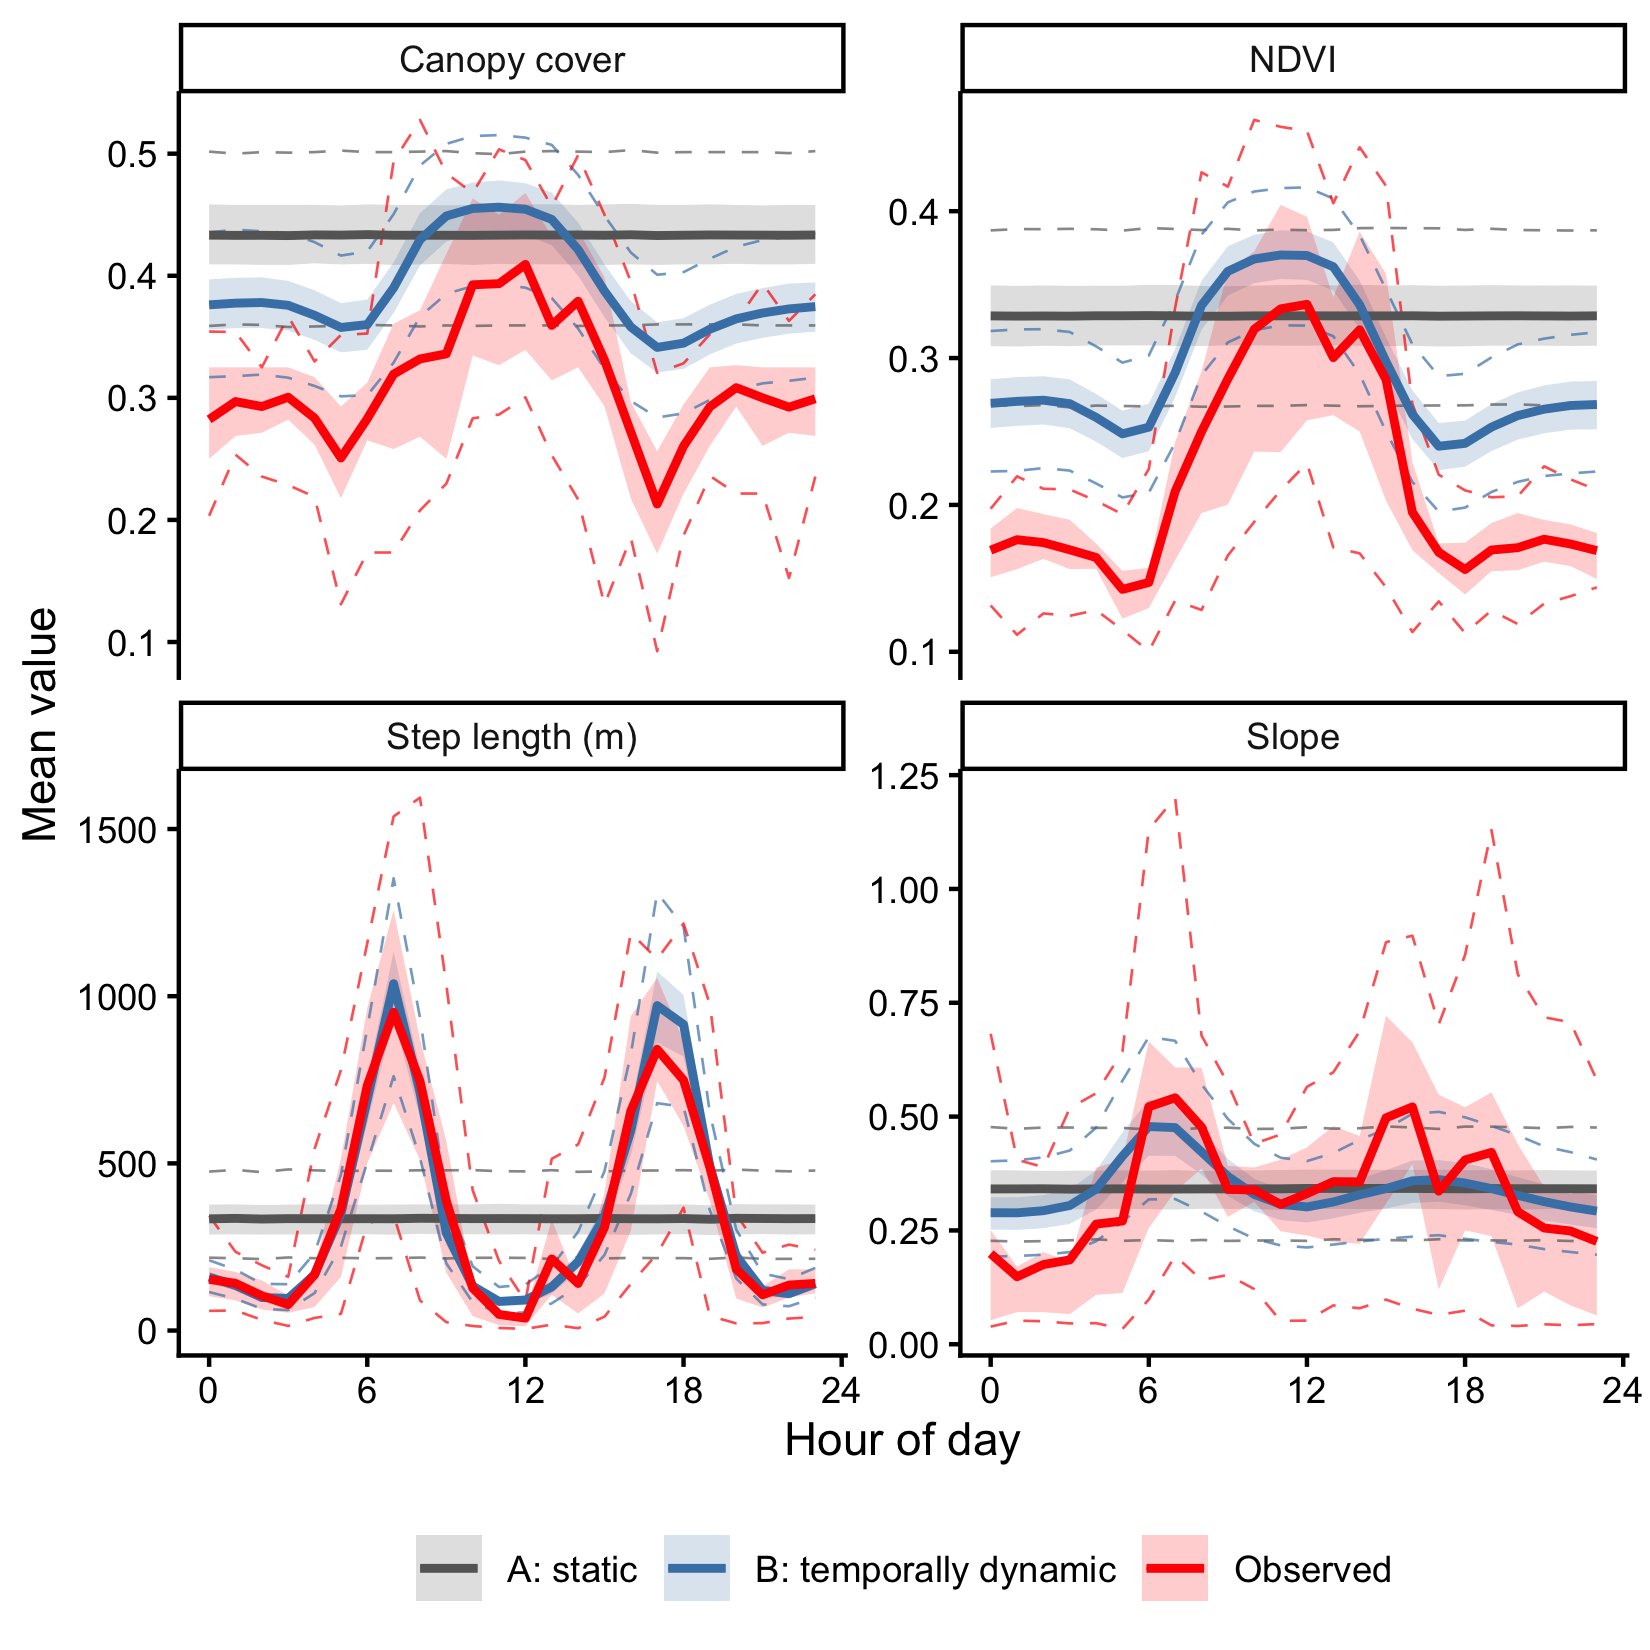
\includegraphics[keepaspectratio]{predictive_SSF_walkthrough_files/figure-pdf/plot_hourly_summaries-1.png}}

}

\caption{Hourly mean step length and habitat use. Ribbons show the 50\%
interval across simulated trajectories (or observed weeks); dashed lines
the 95\% interval; solid lines the mean.}

\end{figure}%

The static model produces flat lines for everything, which is the only
thing it can do. The dynamic model tracks the shape of the observed
daily cycles. The match is not perfect --- the simulated animals roam
over the whole landscape while the observed animal was confined to part
of it, so the absolute levels differ --- but the \emph{timing} of
activity and habitat use is recovered.

\section{11. Assessing the predictions}\label{assessing-the-predictions}

Finally, the question the whole pipeline was built to answer: do the
predicted utilisation distributions match where the animal actually was?

\subsection{The Boyce index}\label{the-boyce-index}

For presence-only data the standard tool is the \textbf{continuous Boyce
index} (Boyce et al. 2002; Hirzel et al. 2006). It divides the range of
predicted values into overlapping bins and, for each, computes the ratio
of observed locations to the area available at that predicted value. For
a good model this ratio increases monotonically with the prediction:
places predicted to be used more, are used more.

The index itself is the rank (Spearman) correlation between that ratio
and the predicted value. It ranges from −1 to 1, where values near zero
indicate a model no better than random.

\begin{Shaded}
\begin{Highlighting}[]
\CommentTok{\#\textquotesingle{} Compute Boyce index statistics for a predicted surface}
\CommentTok{\#\textquotesingle{}}
\CommentTok{\#\textquotesingle{} @param ud  predicted utilisation distribution}
\CommentTok{\#\textquotesingle{} @param obs two{-}column matrix of observed locations}
\NormalTok{compute\_boyce }\OtherTok{\textless{}{-}} \ControlFlowTok{function}\NormalTok{(ud, obs) \{}

  \CommentTok{\# Predicted values at the observed locations}
\NormalTok{  obs\_vals }\OtherTok{\textless{}{-}}\NormalTok{ terra}\SpecialCharTok{::}\FunctionTok{extract}\NormalTok{(ud, obs)[, }\DecValTok{1}\NormalTok{]}
\NormalTok{  obs\_vals }\OtherTok{\textless{}{-}}\NormalTok{ obs\_vals[}\SpecialCharTok{!}\FunctionTok{is.na}\NormalTok{(obs\_vals)]}

  \CommentTok{\# Predicted values across the whole landscape (the "available" set)}
\NormalTok{  all\_vals }\OtherTok{\textless{}{-}}\NormalTok{ terra}\SpecialCharTok{::}\FunctionTok{values}\NormalTok{(ud, }\AttributeTok{na.rm =} \ConstantTok{TRUE}\NormalTok{)[, }\DecValTok{1}\NormalTok{]}
\NormalTok{  all\_vals }\OtherTok{\textless{}{-}}\NormalTok{ all\_vals[}\SpecialCharTok{!}\FunctionTok{is.na}\NormalTok{(all\_vals)]}

  \CommentTok{\# With few observed locations {-} which can happen for a single hour of the day {-}}
  \CommentTok{\# the index is not meaningful, so return NA rather than a misleading number}
  \ControlFlowTok{if}\NormalTok{ (}\FunctionTok{length}\NormalTok{(obs\_vals) }\SpecialCharTok{\textless{}} \DecValTok{10} \SpecialCharTok{||} \FunctionTok{length}\NormalTok{(}\FunctionTok{unique}\NormalTok{(all\_vals)) }\SpecialCharTok{\textless{}} \DecValTok{10}\NormalTok{) \{}
    \FunctionTok{return}\NormalTok{(}\FunctionTok{list}\NormalTok{(}\AttributeTok{spearman =} \ConstantTok{NA\_real\_}\NormalTok{, }\AttributeTok{pearson =} \ConstantTok{NA\_real\_}\NormalTok{,}
                \AttributeTok{F\_ratio =} \FunctionTok{data.frame}\NormalTok{(}\AttributeTok{HS =} \FunctionTok{numeric}\NormalTok{(}\DecValTok{0}\NormalTok{), }\AttributeTok{F.ratio =} \FunctionTok{numeric}\NormalTok{(}\DecValTok{0}\NormalTok{))))}
\NormalTok{  \}}

\NormalTok{  window\_width }\OtherTok{\textless{}{-}}\NormalTok{ (}\FunctionTok{max}\NormalTok{(all\_vals) }\SpecialCharTok{{-}} \FunctionTok{min}\NormalTok{(all\_vals)) }\SpecialCharTok{/} \DecValTok{10}

\NormalTok{  safe\_boyce }\OtherTok{\textless{}{-}} \ControlFlowTok{function}\NormalTok{(method) \{}
\NormalTok{    out }\OtherTok{\textless{}{-}} \FunctionTok{try}\NormalTok{(ecospat}\SpecialCharTok{::}\FunctionTok{ecospat.boyce}\NormalTok{(all\_vals, obs\_vals,}
                                      \AttributeTok{window.w =}\NormalTok{ window\_width, }\AttributeTok{res =} \DecValTok{100}\NormalTok{,}
                                      \AttributeTok{method =}\NormalTok{ method, }\AttributeTok{PEplot =} \ConstantTok{FALSE}\NormalTok{),}
               \AttributeTok{silent =} \ConstantTok{TRUE}\NormalTok{)}
    \ControlFlowTok{if}\NormalTok{ (}\FunctionTok{inherits}\NormalTok{(out, }\StringTok{"try{-}error"}\NormalTok{)) }\ConstantTok{NULL} \ControlFlowTok{else}\NormalTok{ out}
\NormalTok{  \}}

\NormalTok{  bi\_spearman }\OtherTok{\textless{}{-}} \FunctionTok{safe\_boyce}\NormalTok{(}\StringTok{"spearman"}\NormalTok{)}
\NormalTok{  bi\_pearson  }\OtherTok{\textless{}{-}} \FunctionTok{safe\_boyce}\NormalTok{(}\StringTok{"pearson"}\NormalTok{)}

  \FunctionTok{list}\NormalTok{(}
    \AttributeTok{spearman =} \ControlFlowTok{if}\NormalTok{ (}\FunctionTok{is.null}\NormalTok{(bi\_spearman)) }\ConstantTok{NA\_real\_} \ControlFlowTok{else}\NormalTok{ bi\_spearman}\SpecialCharTok{$}\NormalTok{cor,}
    \AttributeTok{pearson  =} \ControlFlowTok{if}\NormalTok{ (}\FunctionTok{is.null}\NormalTok{(bi\_pearson))  }\ConstantTok{NA\_real\_} \ControlFlowTok{else}\NormalTok{ bi\_pearson}\SpecialCharTok{$}\NormalTok{cor,}
    \AttributeTok{F\_ratio  =} \ControlFlowTok{if}\NormalTok{ (}\FunctionTok{is.null}\NormalTok{(bi\_spearman)) }\FunctionTok{data.frame}\NormalTok{(}\AttributeTok{HS =} \FunctionTok{numeric}\NormalTok{(}\DecValTok{0}\NormalTok{), }\AttributeTok{F.ratio =} \FunctionTok{numeric}\NormalTok{(}\DecValTok{0}\NormalTok{))}
               \ControlFlowTok{else} \FunctionTok{data.frame}\NormalTok{(}\AttributeTok{HS =}\NormalTok{ bi\_spearman}\SpecialCharTok{$}\NormalTok{HS, }\AttributeTok{F.ratio =}\NormalTok{ bi\_spearman}\SpecialCharTok{$}\NormalTok{F.ratio)}
\NormalTok{  )}
\NormalTok{\}}
\end{Highlighting}
\end{Shaded}

\begin{Shaded}
\begin{Highlighting}[]
\NormalTok{obs\_locations }\OtherTok{\textless{}{-}} \FunctionTok{cbind}\NormalTok{(buffalo\_id}\SpecialCharTok{$}\NormalTok{x\_, buffalo\_id}\SpecialCharTok{$}\NormalTok{y\_)}

\NormalTok{boyce\_static  }\OtherTok{\textless{}{-}} \FunctionTok{compute\_boyce}\NormalTok{(ud\_static,  obs\_locations)}
\NormalTok{boyce\_dynamic }\OtherTok{\textless{}{-}} \FunctionTok{compute\_boyce}\NormalTok{(ud\_dynamic, obs\_locations)}

\NormalTok{boyce\_results }\OtherTok{\textless{}{-}} \FunctionTok{tibble}\NormalTok{(}
  \AttributeTok{model    =} \FunctionTok{c}\NormalTok{(}\StringTok{"A: static"}\NormalTok{, }\StringTok{"B: temporally dynamic"}\NormalTok{),}
  \AttributeTok{spearman =} \FunctionTok{c}\NormalTok{(boyce\_static}\SpecialCharTok{$}\NormalTok{spearman, boyce\_dynamic}\SpecialCharTok{$}\NormalTok{spearman),}
  \AttributeTok{pearson  =} \FunctionTok{c}\NormalTok{(boyce\_static}\SpecialCharTok{$}\NormalTok{pearson,  boyce\_dynamic}\SpecialCharTok{$}\NormalTok{pearson)}
\NormalTok{)}

\NormalTok{boyce\_results}
\end{Highlighting}
\end{Shaded}

\begin{verbatim}
# A tibble: 2 x 3
  model                 spearman pearson
  <chr>                    <dbl>   <dbl>
1 A: static                0.636   0.618
2 B: temporally dynamic    0.8     0.758
\end{verbatim}

\subsection{Is that number stable?}\label{is-that-number-stable}

Before reading anything into those figures, we should ask whether they
would come out the same again. The convergence check told us the
utilisation distributions are still noisy, and a Boyce index computed on
a noisy surface is itself noisy.

A cheap way to find out, using only the simulations we already have:
split the trajectories into two halves, build a utilisation distribution
from each, and compute the index separately for both. Two halves of the
same simulation, under the same model, should agree.

\begin{Shaded}
\begin{Highlighting}[]
\NormalTok{split\_half\_boyce }\OtherTok{\textless{}{-}} \FunctionTok{map\_dfr}\NormalTok{(}
  \FunctionTok{list}\NormalTok{(}\StringTok{"A: static"} \OtherTok{=}\NormalTok{ sims\_static, }\StringTok{"B: temporally dynamic"} \OtherTok{=}\NormalTok{ sims\_dynamic),}
  \ControlFlowTok{function}\NormalTok{(sims) \{}
\NormalTok{    half\_1 }\OtherTok{\textless{}{-}}\NormalTok{ sims }\SpecialCharTok{\%\textgreater{}\%} \FunctionTok{filter}\NormalTok{(traj\_id }\SpecialCharTok{\textless{}=}\NormalTok{ n\_traj }\SpecialCharTok{/} \DecValTok{2}\NormalTok{)}
\NormalTok{    half\_2 }\OtherTok{\textless{}{-}}\NormalTok{ sims }\SpecialCharTok{\%\textgreater{}\%} \FunctionTok{filter}\NormalTok{(traj\_id }\SpecialCharTok{\textgreater{}}\NormalTok{  n\_traj }\SpecialCharTok{/} \DecValTok{2}\NormalTok{)}
    \FunctionTok{data.frame}\NormalTok{(}
      \AttributeTok{half\_1 =} \FunctionTok{compute\_boyce}\NormalTok{(}\FunctionTok{aggregate\_to\_ud}\NormalTok{(half\_1, ud\_res), obs\_locations)}\SpecialCharTok{$}\NormalTok{spearman,}
      \AttributeTok{half\_2 =} \FunctionTok{compute\_boyce}\NormalTok{(}\FunctionTok{aggregate\_to\_ud}\NormalTok{(half\_2, ud\_res), obs\_locations)}\SpecialCharTok{$}\NormalTok{spearman}
\NormalTok{    )}
\NormalTok{  \}, }\AttributeTok{.id =} \StringTok{"model"}\NormalTok{) }\SpecialCharTok{\%\textgreater{}\%}
  \FunctionTok{mutate}\NormalTok{(}\AttributeTok{difference =} \FunctionTok{abs}\NormalTok{(half\_1 }\SpecialCharTok{{-}}\NormalTok{ half\_2))}

\NormalTok{split\_half\_boyce}
\end{Highlighting}
\end{Shaded}

\begin{verbatim}
                  model half_1 half_2 difference
1             A: static  0.243  0.723      0.480
2 B: temporally dynamic  0.716  0.501      0.215
\end{verbatim}

The halves agree closely --- to within about 0.01 for the static model.
That looks reassuring.

\textbf{It is misleading}, and the next check shows why. The two halves
are not as independent as they appear: both are drawn under the same
starting locations and the same simulation setup, so they share whatever
that particular run happens to be doing. A split-half check measures
\emph{within-run} sampling noise only.

The check that actually matters is to re-run the whole simulation from
scratch, several times, and see how far the answer moves. That is more
expensive, which is why it is tempting to skip --- so we do it at
reduced scale rather than not at all.

\begin{Shaded}
\begin{Highlighting}[]
\CommentTok{\# Repeat the entire simulation a few times, with independent starting locations}
\CommentTok{\# and independent random draws each time. Reduced scale to keep the runtime}
\CommentTok{\# sensible {-} which, if anything, understates the stability of the full run.}
\NormalTok{n\_repeat      }\OtherTok{\textless{}{-}} \DecValTok{3}
\NormalTok{n\_repeat\_traj }\OtherTok{\textless{}{-}} \DecValTok{200}

\NormalTok{repeat\_runs }\OtherTok{\textless{}{-}} \FunctionTok{map\_dfr}\NormalTok{(}\FunctionTok{seq\_len}\NormalTok{(n\_repeat), }\ControlFlowTok{function}\NormalTok{(rep) \{}
  \FunctionTok{set.seed}\NormalTok{(}\DecValTok{5000} \SpecialCharTok{+}\NormalTok{ rep)}
  \FunctionTok{map\_dfr}\NormalTok{(}
    \FunctionTok{list}\NormalTok{(}\StringTok{"A: static"} \OtherTok{=} \FunctionTok{list}\NormalTok{(}\AttributeTok{lk =}\NormalTok{ lookup\_static,  }\AttributeTok{cf =}\NormalTok{ hourly\_coefs\_static),}
         \StringTok{"B: temporally dynamic"} \OtherTok{=} \FunctionTok{list}\NormalTok{(}\AttributeTok{lk =}\NormalTok{ lookup\_dynamic, }\AttributeTok{cf =}\NormalTok{ hourly\_coefs\_dynamic)),}
    \ControlFlowTok{function}\NormalTok{(m) \{}
\NormalTok{      sims\_rep }\OtherTok{\textless{}{-}} \FunctionTok{run\_simulation\_set}\NormalTok{(}
        \AttributeTok{lk =}\NormalTok{ m}\SpecialCharTok{$}\NormalTok{lk, }\AttributeTok{coefs =}\NormalTok{ m}\SpecialCharTok{$}\NormalTok{cf, }\AttributeTok{mode =} \StringTok{"random"}\NormalTok{,}
        \AttributeTok{n\_traj =}\NormalTok{ n\_repeat\_traj, }\AttributeTok{n\_steps =}\NormalTok{ n\_steps, }\AttributeTok{boundary =} \StringTok{"wrapped"}\NormalTok{,}
        \AttributeTok{label =} \StringTok{"repeat"}\NormalTok{)}
      \FunctionTok{data.frame}\NormalTok{(}
        \AttributeTok{boyce =} \FunctionTok{compute\_boyce}\NormalTok{(}\FunctionTok{aggregate\_to\_ud}\NormalTok{(sims\_rep, ud\_res), obs\_locations)}\SpecialCharTok{$}\NormalTok{spearman}
\NormalTok{      )}
\NormalTok{    \}, }\AttributeTok{.id =} \StringTok{"model"}\NormalTok{) }\SpecialCharTok{\%\textgreater{}\%}
    \FunctionTok{mutate}\NormalTok{(}\AttributeTok{run =}\NormalTok{ rep)}
\NormalTok{\})}
\end{Highlighting}
\end{Shaded}

\begin{verbatim}
Simulating: repeat: 4.583 sec elapsed
Simulating: repeat: 4.338 sec elapsed
Simulating: repeat: 4.371 sec elapsed
Simulating: repeat: 4.529 sec elapsed
Simulating: repeat: 4.437 sec elapsed
Simulating: repeat: 4.815 sec elapsed
\end{verbatim}

\begin{Shaded}
\begin{Highlighting}[]
\NormalTok{repeat\_runs }\SpecialCharTok{\%\textgreater{}\%}
  \FunctionTok{pivot\_wider}\NormalTok{(}\AttributeTok{names\_from =}\NormalTok{ run, }\AttributeTok{values\_from =}\NormalTok{ boyce, }\AttributeTok{names\_prefix =} \StringTok{"run\_"}\NormalTok{) }\SpecialCharTok{\%\textgreater{}\%}
  \FunctionTok{rowwise}\NormalTok{() }\SpecialCharTok{\%\textgreater{}\%}
  \FunctionTok{mutate}\NormalTok{(}\AttributeTok{spread =} \FunctionTok{max}\NormalTok{(}\FunctionTok{c\_across}\NormalTok{(}\FunctionTok{starts\_with}\NormalTok{(}\StringTok{"run\_"}\NormalTok{))) }\SpecialCharTok{{-}}
                  \FunctionTok{min}\NormalTok{(}\FunctionTok{c\_across}\NormalTok{(}\FunctionTok{starts\_with}\NormalTok{(}\StringTok{"run\_"}\NormalTok{)))) }\SpecialCharTok{\%\textgreater{}\%}
  \FunctionTok{ungroup}\NormalTok{()}
\end{Highlighting}
\end{Shaded}

\begin{verbatim}
# A tibble: 2 x 5
  model                  run_1 run_2  run_3 spread
  <chr>                  <dbl> <dbl>  <dbl>  <dbl>
1 A: static             -0.284 0.808 -0.461  1.27 
2 B: temporally dynamic  0.879 0.768  0.628  0.251
\end{verbatim}

\begin{tcolorbox}[enhanced jigsaw, arc=.35mm, bottomrule=.15mm, bottomtitle=1mm, breakable, colback=white, colbacktitle=quarto-callout-important-color!10!white, colframe=quarto-callout-important-color-frame, coltitle=black, left=2mm, leftrule=.75mm, opacityback=0, opacitybacktitle=0.6, rightrule=.15mm, title=\textcolor{quarto-callout-important-color}{\faExclamation}\hspace{0.5em}{A split-half check is necessary but nowhere near sufficient}, titlerule=0mm, toprule=.15mm, toptitle=1mm]

Compare the two tables. Split-half agreement suggested the static
model's index was stable to about \textbf{±0.01}. Repeating the
simulation from scratch moves it by far more than that.

Running this at the full 1000 trajectories, five times per model, gives
the picture clearly:

{\def\LTcaptype{none} % do not increment counter
\begin{longtable}[]{@{}lllll@{}}
\toprule\noalign{}
Model & mean & sd & min & max \\
\midrule\noalign{}
\endhead
\bottomrule\noalign{}
\endlastfoot
A: static & 0.524 & \textbf{0.350} & −0.040 & 0.840 \\
B: temporally dynamic & 0.773 & 0.118 & 0.632 & 0.909 \\
\end{longtable}
}

The static model's whole-day Boyce index is essentially uninformative
from any single run: five independent runs of the \emph{identical} model
on the \emph{identical} data returned values spanning −0.04 to 0.84. The
split-half check understated that variability by a factor of roughly
thirty.

This is not hypothetical. An earlier version of this walkthrough drew
turning angles with \texttt{Rfast::rvonmises()}; on that run the static
model scored \textbf{0.729} here instead of the value above. Nothing
about the model or the data changed --- only the random draws. Both
numbers sit comfortably inside the range above.

Why the static model in particular: its habitat coefficients are small,
so its selection surface is nearly flat, the simulated animals wander
close to uniformly, and the resulting utilisation distribution carries
little signal for the index to latch onto. The dynamic model's surface
has real structure, so its estimate is correspondingly better determined
(sd 0.118).

Two things follow. \textbf{On average the dynamic model does score
higher on this comparison} (0.773 vs 0.524) --- but you could not have
learned that from one run, and a single run is what most analyses
report. And the honest conclusion from the single-run table above is not
a ranking at all; it is that the whole-day comparison needs far more
trajectories before it can support one.

\end{tcolorbox}

\begin{Shaded}
\begin{Highlighting}[]
\FunctionTok{bind\_rows}\NormalTok{(}
\NormalTok{  boyce\_static}\SpecialCharTok{$}\NormalTok{F\_ratio  }\SpecialCharTok{\%\textgreater{}\%} \FunctionTok{mutate}\NormalTok{(}\AttributeTok{model =} \StringTok{"A: static"}\NormalTok{),}
\NormalTok{  boyce\_dynamic}\SpecialCharTok{$}\NormalTok{F\_ratio }\SpecialCharTok{\%\textgreater{}\%} \FunctionTok{mutate}\NormalTok{(}\AttributeTok{model =} \StringTok{"B: temporally dynamic"}\NormalTok{)}
\NormalTok{) }\SpecialCharTok{\%\textgreater{}\%}
  \FunctionTok{ggplot}\NormalTok{(}\FunctionTok{aes}\NormalTok{(}\AttributeTok{x =}\NormalTok{ HS, }\AttributeTok{y =}\NormalTok{ F.ratio, }\AttributeTok{colour =}\NormalTok{ model)) }\SpecialCharTok{+}
  \FunctionTok{geom\_hline}\NormalTok{(}\AttributeTok{yintercept =} \DecValTok{1}\NormalTok{, }\AttributeTok{linetype =} \StringTok{"dashed"}\NormalTok{, }\AttributeTok{colour =} \StringTok{"grey40"}\NormalTok{) }\SpecialCharTok{+}
  \FunctionTok{geom\_line}\NormalTok{(}\AttributeTok{linewidth =} \FloatTok{0.9}\NormalTok{) }\SpecialCharTok{+}
  \FunctionTok{scale\_colour\_manual}\NormalTok{(}\AttributeTok{values =}\NormalTok{ model\_colours, }\AttributeTok{name =} \ConstantTok{NULL}\NormalTok{) }\SpecialCharTok{+}
  \FunctionTok{scale\_x\_continuous}\NormalTok{(}\StringTok{"Predicted use (normalised)"}\NormalTok{) }\SpecialCharTok{+}
  \FunctionTok{scale\_y\_log10}\NormalTok{(}\StringTok{"Predicted{-}to{-}expected ratio"}\NormalTok{) }\SpecialCharTok{+}
  \FunctionTok{theme\_classic}\NormalTok{() }\SpecialCharTok{+}
  \FunctionTok{theme}\NormalTok{(}\AttributeTok{legend.position =} \StringTok{"bottom"}\NormalTok{)}
\end{Highlighting}
\end{Shaded}

\begin{figure}[H]

{\centering \pandocbounded{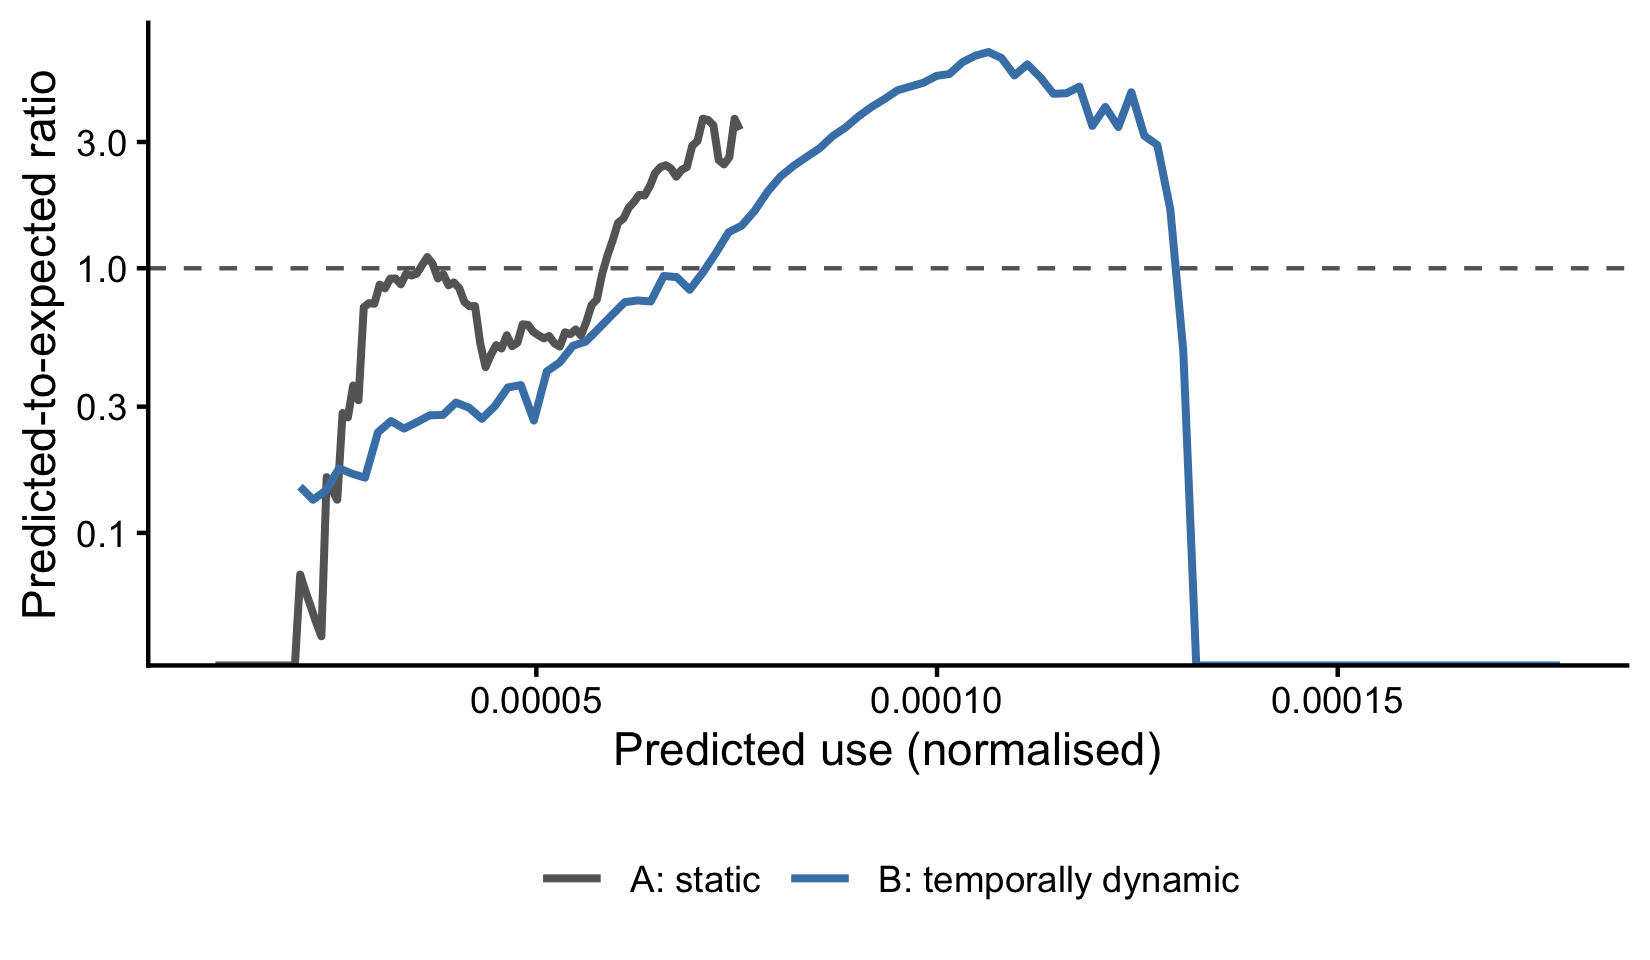
\includegraphics[keepaspectratio]{predictive_SSF_walkthrough_files/figure-pdf/plot_f_ratio-1.png}}

}

\caption{Predicted-to-expected ratio against predicted habitat
suitability. A well-calibrated model rises monotonically above the
dashed line at 1.}

\end{figure}%

The F-ratio curve is more informative than the single index value,
because it shows \emph{where} a model succeeds or fails. A model can
achieve a respectable correlation while badly over-predicting use in the
very highest-suitability cells, and that shows up here as a curve that
flattens or turns down at the right-hand end.

\subsection{Correlation with a kernel density
estimate}\label{correlation-with-a-kernel-density-estimate}

A complementary check: compare the predicted UD against a kernel density
estimate of the observed locations, which gives a smooth empirical
surface rather than a set of points.

\begin{Shaded}
\begin{Highlighting}[]
\CommentTok{\# Kernel density estimate of the observed locations, on the same grid as the}
\CommentTok{\# predicted UDs so the two can be compared cell by cell}
\NormalTok{kde\_template }\OtherTok{\textless{}{-}} \FunctionTok{rast}\NormalTok{(}\AttributeTok{extent =} \FunctionTok{ext}\NormalTok{(ndvi\_crop), }\AttributeTok{resolution =}\NormalTok{ ud\_res, }\AttributeTok{crs =} \FunctionTok{crs}\NormalTok{(ndvi\_crop))}

\NormalTok{obs\_kde }\OtherTok{\textless{}{-}} \FunctionTok{hr\_kde}\NormalTok{(buffalo\_id, }\AttributeTok{trast =}\NormalTok{ kde\_template)}

\CommentTok{\# Normalise to sum to 1, matching the predicted UDs. Kernel density estimation}
\CommentTok{\# can return tiny negative values through numerical error, so clamp at zero first.}
\NormalTok{kde\_rast }\OtherTok{\textless{}{-}}\NormalTok{ obs\_kde}\SpecialCharTok{$}\NormalTok{ud}
\NormalTok{kde\_rast[kde\_rast }\SpecialCharTok{\textless{}} \DecValTok{0}\NormalTok{] }\OtherTok{\textless{}{-}} \DecValTok{0}
\NormalTok{kde\_rast }\OtherTok{\textless{}{-}}\NormalTok{ kde\_rast }\SpecialCharTok{/} \FunctionTok{global}\NormalTok{(kde\_rast, }\StringTok{"sum"}\NormalTok{, }\AttributeTok{na.rm =} \ConstantTok{TRUE}\NormalTok{)[[}\DecValTok{1}\NormalTok{]]}

\NormalTok{kde\_correlations }\OtherTok{\textless{}{-}} \FunctionTok{tibble}\NormalTok{(}
  \AttributeTok{model =} \FunctionTok{c}\NormalTok{(}\StringTok{"A: static"}\NormalTok{, }\StringTok{"B: temporally dynamic"}\NormalTok{),}
  \AttributeTok{spearman\_vs\_kde =} \FunctionTok{c}\NormalTok{(}
    \FunctionTok{cor}\NormalTok{(}\FunctionTok{values}\NormalTok{(ud\_static)[, }\DecValTok{1}\NormalTok{],  }\FunctionTok{values}\NormalTok{(kde\_rast)[, }\DecValTok{1}\NormalTok{],}
        \AttributeTok{use =} \StringTok{"complete.obs"}\NormalTok{, }\AttributeTok{method =} \StringTok{"spearman"}\NormalTok{),}
    \FunctionTok{cor}\NormalTok{(}\FunctionTok{values}\NormalTok{(ud\_dynamic)[, }\DecValTok{1}\NormalTok{], }\FunctionTok{values}\NormalTok{(kde\_rast)[, }\DecValTok{1}\NormalTok{],}
        \AttributeTok{use =} \StringTok{"complete.obs"}\NormalTok{, }\AttributeTok{method =} \StringTok{"spearman"}\NormalTok{)}
\NormalTok{  )}
\NormalTok{)}

\NormalTok{kde\_correlations}
\end{Highlighting}
\end{Shaded}

\begin{verbatim}
# A tibble: 2 x 2
  model                 spearman_vs_kde
  <chr>                           <dbl>
1 A: static                      0.0414
2 B: temporally dynamic          0.251 
\end{verbatim}

\begin{Shaded}
\begin{Highlighting}[]
\NormalTok{kde\_df }\OtherTok{\textless{}{-}} \FunctionTok{as.data.frame}\NormalTok{(kde\_rast, }\AttributeTok{xy =} \ConstantTok{TRUE}\NormalTok{)}
\FunctionTok{names}\NormalTok{(kde\_df)[}\DecValTok{3}\NormalTok{] }\OtherTok{\textless{}{-}} \StringTok{"density"}

\NormalTok{p\_kde }\OtherTok{\textless{}{-}} \FunctionTok{ggplot}\NormalTok{(kde\_df, }\FunctionTok{aes}\NormalTok{(}\AttributeTok{x =}\NormalTok{ x, }\AttributeTok{y =}\NormalTok{ y, }\AttributeTok{fill =} \FunctionTok{log10}\NormalTok{(density }\SpecialCharTok{+} \FloatTok{1e{-}8}\NormalTok{))) }\SpecialCharTok{+}
  \FunctionTok{geom\_raster}\NormalTok{() }\SpecialCharTok{+}
  \FunctionTok{scale\_fill\_viridis\_c}\NormalTok{(}\StringTok{"log10}\SpecialCharTok{\textbackslash{}n}\StringTok{density"}\NormalTok{, }\AttributeTok{option =} \StringTok{"magma"}\NormalTok{) }\SpecialCharTok{+}
  \FunctionTok{coord\_equal}\NormalTok{() }\SpecialCharTok{+}
  \FunctionTok{labs}\NormalTok{(}\AttributeTok{title =} \StringTok{"Observed (KDE)"}\NormalTok{, }\AttributeTok{x =} \ConstantTok{NULL}\NormalTok{, }\AttributeTok{y =} \ConstantTok{NULL}\NormalTok{) }\SpecialCharTok{+}
  \FunctionTok{theme\_classic}\NormalTok{() }\SpecialCharTok{+}
  \FunctionTok{theme}\NormalTok{(}\AttributeTok{axis.text =} \FunctionTok{element\_text}\NormalTok{(}\AttributeTok{size =} \DecValTok{6}\NormalTok{), }\AttributeTok{plot.title =} \FunctionTok{element\_text}\NormalTok{(}\AttributeTok{size =} \DecValTok{10}\NormalTok{))}

\NormalTok{p\_kde }\SpecialCharTok{+} \FunctionTok{plot\_ud}\NormalTok{(ud\_dynamic, }\StringTok{"Predicted (dynamic model)"}\NormalTok{)}
\end{Highlighting}
\end{Shaded}

\begin{figure}[H]

{\centering \pandocbounded{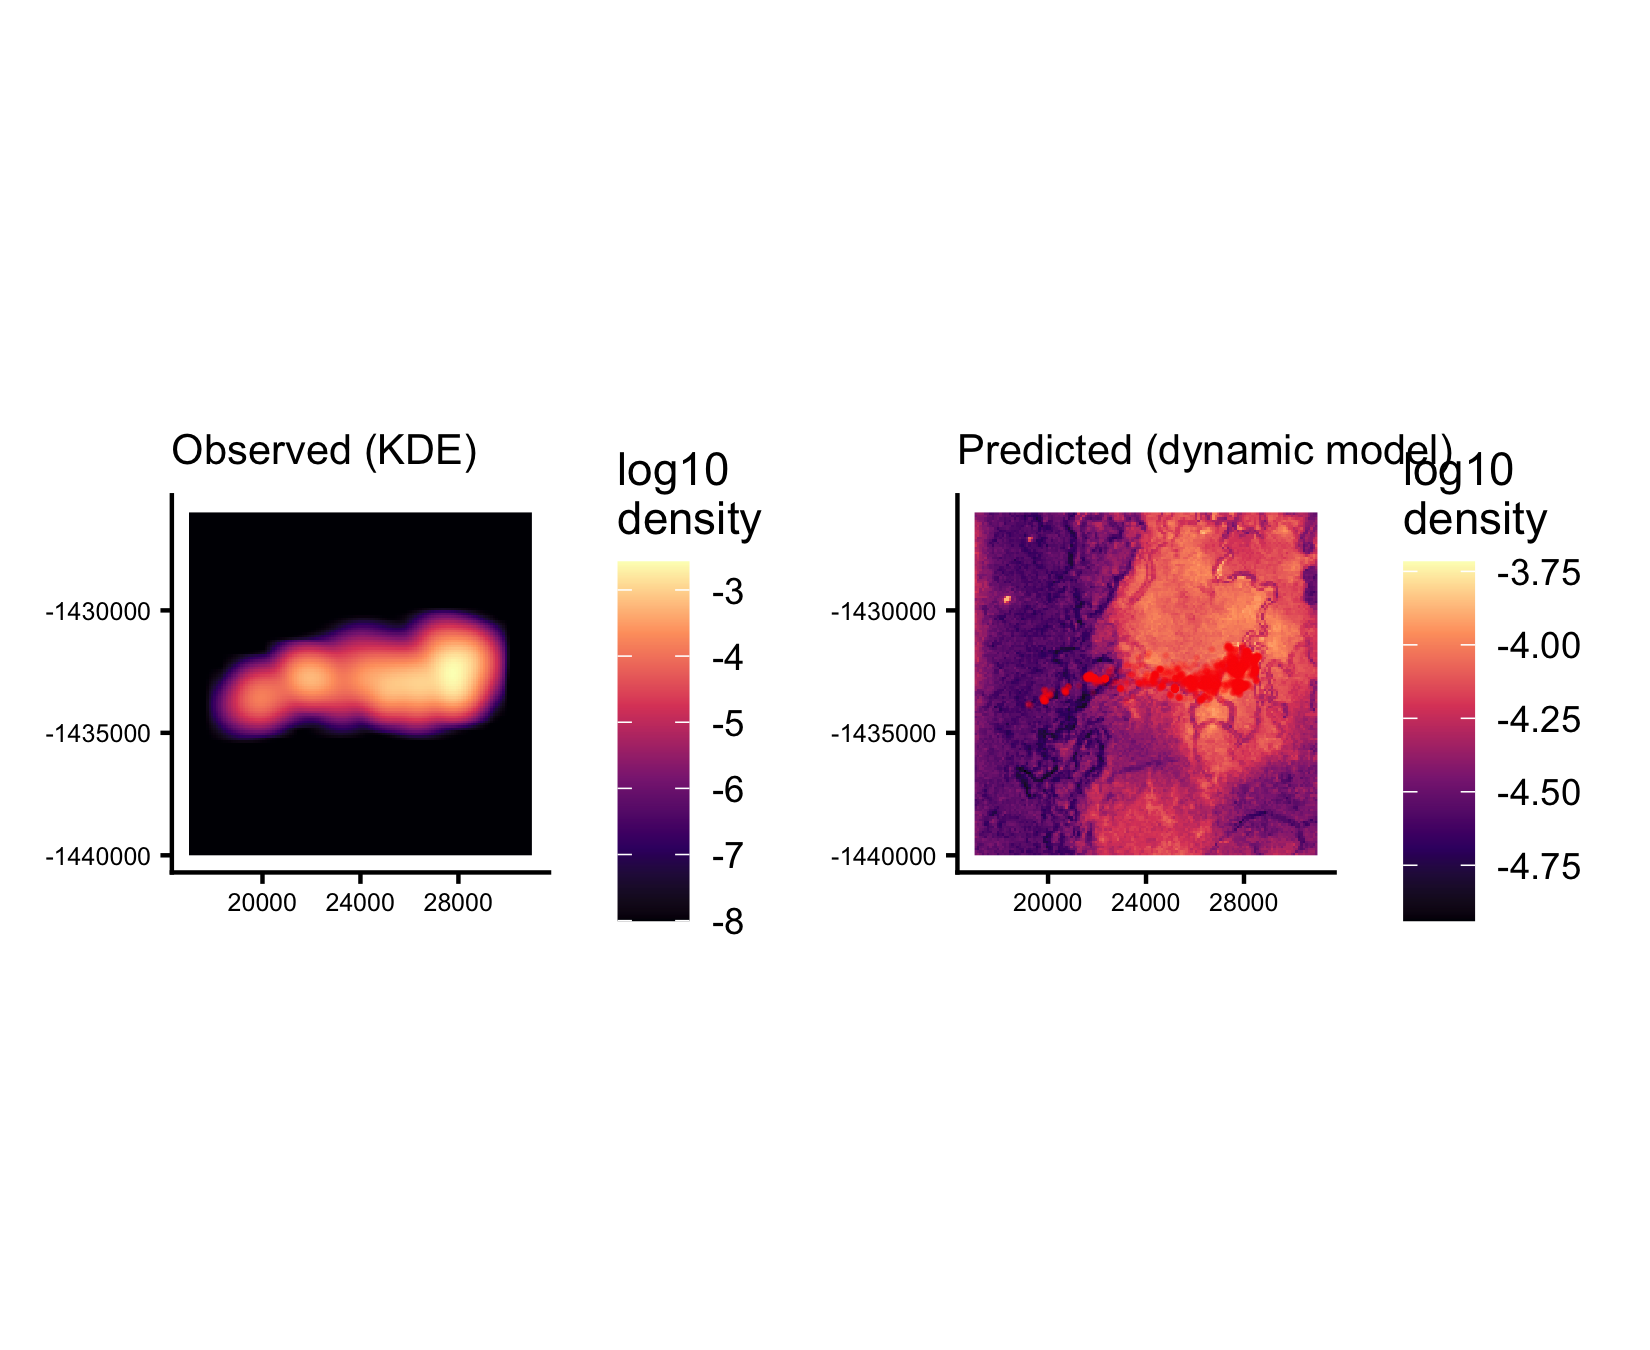
\includegraphics[keepaspectratio]{predictive_SSF_walkthrough_files/figure-pdf/kde_comparison-1.png}}

}

\caption{Observed kernel density estimate alongside the dynamic model's
prediction.}

\end{figure}%

\subsection{Validation by hour of day}\label{validation-by-hour-of-day}

The overall UD averages over the day, which is precisely the comparison
least likely to reveal an advantage for the dynamic model. The sharper
test is hour by hour: for each hour, we compare that hour's predicted UD
against the locations the animal actually occupied at that hour.

\begin{Shaded}
\begin{Highlighting}[]
\NormalTok{observed\_by\_hour }\OtherTok{\textless{}{-}}\NormalTok{ buffalo\_id }\SpecialCharTok{\%\textgreater{}\%} \FunctionTok{mutate}\NormalTok{(}\AttributeTok{hour =} \FunctionTok{hour}\NormalTok{(t\_))}

\NormalTok{hourly\_validation }\OtherTok{\textless{}{-}} \FunctionTok{map\_dfr}\NormalTok{(}\DecValTok{0}\SpecialCharTok{:}\DecValTok{23}\NormalTok{, }\ControlFlowTok{function}\NormalTok{(h) \{}

\NormalTok{  obs\_h }\OtherTok{\textless{}{-}}\NormalTok{ observed\_by\_hour }\SpecialCharTok{\%\textgreater{}\%} \FunctionTok{filter}\NormalTok{(hour }\SpecialCharTok{==}\NormalTok{ h)}
\NormalTok{  obs\_h\_mat }\OtherTok{\textless{}{-}} \FunctionTok{cbind}\NormalTok{(obs\_h}\SpecialCharTok{$}\NormalTok{x\_, obs\_h}\SpecialCharTok{$}\NormalTok{y\_)}

\NormalTok{  bi\_static  }\OtherTok{\textless{}{-}} \FunctionTok{compute\_boyce}\NormalTok{(uds\_hourly\_static[[h }\SpecialCharTok{+} \DecValTok{1}\NormalTok{]],  obs\_h\_mat)}
\NormalTok{  bi\_dynamic }\OtherTok{\textless{}{-}} \FunctionTok{compute\_boyce}\NormalTok{(uds\_hourly\_dynamic[[h }\SpecialCharTok{+} \DecValTok{1}\NormalTok{]], obs\_h\_mat)}

  \FunctionTok{data.frame}\NormalTok{(}
    \AttributeTok{hour =}\NormalTok{ h,}
    \AttributeTok{n\_observed =} \FunctionTok{nrow}\NormalTok{(obs\_h),}
    \StringTok{\textasciigrave{}}\AttributeTok{A: static}\StringTok{\textasciigrave{}} \OtherTok{=}\NormalTok{ bi\_static}\SpecialCharTok{$}\NormalTok{spearman,}
    \StringTok{\textasciigrave{}}\AttributeTok{B: temporally dynamic}\StringTok{\textasciigrave{}} \OtherTok{=}\NormalTok{ bi\_dynamic}\SpecialCharTok{$}\NormalTok{spearman,}
    \AttributeTok{check.names =} \ConstantTok{FALSE}
\NormalTok{  )}
\NormalTok{\})}

\NormalTok{hourly\_validation}
\end{Highlighting}
\end{Shaded}

\begin{verbatim}
   hour n_observed A: static B: temporally dynamic
1     0         97     0.683                 0.879
2     1         98     0.677                 0.892
3     2         98     0.470                 0.951
4     3         98     0.814                 0.922
5     4         98     0.575                 0.742
6     5         98     0.683                 0.776
7     6         98     0.739                 0.804
8     7         97     0.805                 0.853
9     8         88     0.770                 0.629
10    9         90     0.206                 0.736
11   10         95     0.024                 0.726
12   11         97     0.087                 0.551
13   12         93    -0.438                 0.615
14   13         95    -0.028                 0.761
15   14         69     0.188                 0.702
16   15         63     0.186                 0.706
17   16         87     0.171                 0.533
18   17         96     0.259                 0.423
19   18         93     0.508                 0.626
20   19         96     0.170                 0.866
21   20         96     0.151                 0.731
22   21         97     0.475                 0.739
23   22         99     0.188                 0.820
24   23         99    -0.037                 0.867
\end{verbatim}

\begin{Shaded}
\begin{Highlighting}[]
\NormalTok{hourly\_validation }\SpecialCharTok{\%\textgreater{}\%}
  \FunctionTok{pivot\_longer}\NormalTok{(}\FunctionTok{c}\NormalTok{(}\StringTok{\textasciigrave{}}\AttributeTok{A: static}\StringTok{\textasciigrave{}}\NormalTok{, }\StringTok{\textasciigrave{}}\AttributeTok{B: temporally dynamic}\StringTok{\textasciigrave{}}\NormalTok{),}
               \AttributeTok{names\_to =} \StringTok{"model"}\NormalTok{, }\AttributeTok{values\_to =} \StringTok{"boyce"}\NormalTok{) }\SpecialCharTok{\%\textgreater{}\%}
  \FunctionTok{ggplot}\NormalTok{(}\FunctionTok{aes}\NormalTok{(}\AttributeTok{x =}\NormalTok{ hour, }\AttributeTok{y =}\NormalTok{ boyce, }\AttributeTok{colour =}\NormalTok{ model)) }\SpecialCharTok{+}
  \FunctionTok{geom\_hline}\NormalTok{(}\AttributeTok{yintercept =} \DecValTok{0}\NormalTok{, }\AttributeTok{linetype =} \StringTok{"dashed"}\NormalTok{, }\AttributeTok{colour =} \StringTok{"grey40"}\NormalTok{) }\SpecialCharTok{+}
  \FunctionTok{geom\_line}\NormalTok{(}\AttributeTok{linewidth =} \FloatTok{0.9}\NormalTok{) }\SpecialCharTok{+}
  \FunctionTok{geom\_point}\NormalTok{(}\AttributeTok{size =} \FloatTok{1.5}\NormalTok{) }\SpecialCharTok{+}
  \FunctionTok{scale\_colour\_manual}\NormalTok{(}\AttributeTok{values =}\NormalTok{ model\_colours, }\AttributeTok{name =} \ConstantTok{NULL}\NormalTok{) }\SpecialCharTok{+}
  \FunctionTok{scale\_x\_continuous}\NormalTok{(}\StringTok{"Hour of day"}\NormalTok{, }\AttributeTok{breaks =} \FunctionTok{seq}\NormalTok{(}\DecValTok{0}\NormalTok{, }\DecValTok{24}\NormalTok{, }\DecValTok{6}\NormalTok{)) }\SpecialCharTok{+}
  \FunctionTok{scale\_y\_continuous}\NormalTok{(}\StringTok{"Continuous Boyce index"}\NormalTok{) }\SpecialCharTok{+}
  \FunctionTok{theme\_classic}\NormalTok{() }\SpecialCharTok{+}
  \FunctionTok{theme}\NormalTok{(}\AttributeTok{legend.position =} \StringTok{"bottom"}\NormalTok{)}
\end{Highlighting}
\end{Shaded}

\begin{figure}[H]

{\centering \pandocbounded{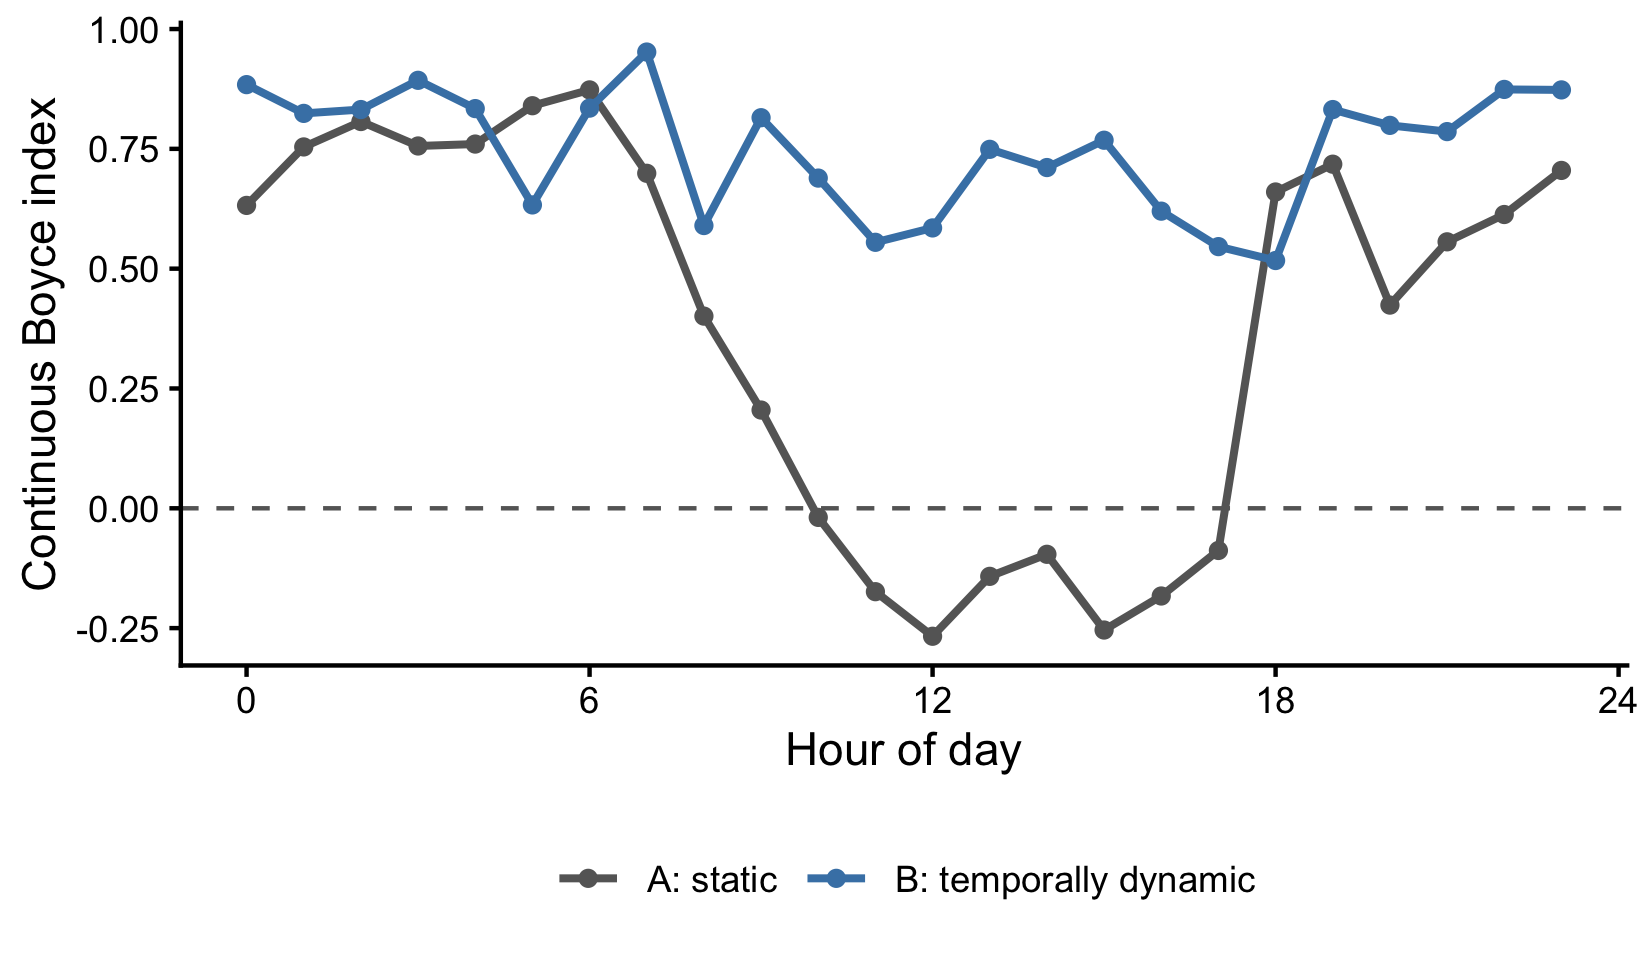
\includegraphics[keepaspectratio]{predictive_SSF_walkthrough_files/figure-pdf/plot_hourly_validation-1.png}}

}

\caption{Continuous Boyce index by hour of day for each model.}

\end{figure}%

\begin{Shaded}
\begin{Highlighting}[]
\NormalTok{hourly\_validation }\SpecialCharTok{\%\textgreater{}\%}
  \FunctionTok{summarise}\NormalTok{(}
    \AttributeTok{mean\_static  =} \FunctionTok{mean}\NormalTok{(}\StringTok{\textasciigrave{}}\AttributeTok{A: static}\StringTok{\textasciigrave{}}\NormalTok{, }\AttributeTok{na.rm =} \ConstantTok{TRUE}\NormalTok{),}
    \AttributeTok{mean\_dynamic =} \FunctionTok{mean}\NormalTok{(}\StringTok{\textasciigrave{}}\AttributeTok{B: temporally dynamic}\StringTok{\textasciigrave{}}\NormalTok{, }\AttributeTok{na.rm =} \ConstantTok{TRUE}\NormalTok{),}
    \AttributeTok{hours\_dynamic\_better =} \FunctionTok{sum}\NormalTok{(}\StringTok{\textasciigrave{}}\AttributeTok{B: temporally dynamic}\StringTok{\textasciigrave{}} \SpecialCharTok{\textgreater{}} \StringTok{\textasciigrave{}}\AttributeTok{A: static}\StringTok{\textasciigrave{}}\NormalTok{, }\AttributeTok{na.rm =} \ConstantTok{TRUE}\NormalTok{),}
    \AttributeTok{hours\_compared =} \FunctionTok{sum}\NormalTok{(}\SpecialCharTok{!}\FunctionTok{is.na}\NormalTok{(}\StringTok{\textasciigrave{}}\AttributeTok{A: static}\StringTok{\textasciigrave{}}\NormalTok{) }\SpecialCharTok{\&} \SpecialCharTok{!}\FunctionTok{is.na}\NormalTok{(}\StringTok{\textasciigrave{}}\AttributeTok{B: temporally dynamic}\StringTok{\textasciigrave{}}\NormalTok{))}
\NormalTok{  )}
\end{Highlighting}
\end{Shaded}

\begin{verbatim}
  mean_static mean_dynamic hours_dynamic_better hours_compared
1   0.3469167      0.74375                   23             24
\end{verbatim}

This is the comparison the temporally dynamic approach is built for, and
it is a miniature version of the central result in Forrest et al.
(2025). The dynamic model scores substantially higher in the large
majority of hours.

Two caveats keep this honest. First, these hourly distributions are
built from a \emph{fraction} of the simulated locations that the
whole-day one used, so they are noisier still --- the gap is large and
consistent across hours, which is why it is worth reporting, but the
individual hourly values are not precise. Second, this is not an
out-of-sample test: the models were fitted to these same observed
locations, so what we are checking is whether a fitted model can
reproduce the pattern it was fitted to, not whether it would predict a
held-out period or a different animal.

With those caveats, the direction of the result is what the model
structure predicts. The static model cannot represent a daily cycle at
all, so it has one map to offer for every hour; the dynamic model has
twenty-four, and the animal's location does in fact depend on the hour.

\section{\texorpdfstring{12. Doing the same thing with
\texttt{amt}}{12. Doing the same thing with amt}}\label{doing-the-same-thing-with-amt}

Everything above simulates by hand, so that each part of the
redistribution kernel is visible. In practice, \texttt{amt} implements
this directly (Signer et al. 2023), and for a static model you can go
from a fitted object to simulated paths in a few lines.

\begin{Shaded}
\begin{Highlighting}[]
\CommentTok{\# The movement distributions amt derives from the fitted model {-} these should}
\CommentTok{\# match the values we computed by hand in section 6}
\NormalTok{amt\_sl\_distr }\OtherTok{\textless{}{-}}\NormalTok{ amt}\SpecialCharTok{::}\FunctionTok{update\_sl\_distr}\NormalTok{(ssf\_static)}
\NormalTok{amt\_ta\_distr }\OtherTok{\textless{}{-}}\NormalTok{ amt}\SpecialCharTok{::}\FunctionTok{update\_ta\_distr}\NormalTok{(ssf\_static)}

\FunctionTok{cat}\NormalTok{(}\StringTok{"amt    {-} shape:"}\NormalTok{, }\FunctionTok{round}\NormalTok{(amt\_sl\_distr}\SpecialCharTok{$}\NormalTok{params}\SpecialCharTok{$}\NormalTok{shape, }\DecValTok{6}\NormalTok{),}
    \StringTok{" scale:"}\NormalTok{, }\FunctionTok{round}\NormalTok{(amt\_sl\_distr}\SpecialCharTok{$}\NormalTok{params}\SpecialCharTok{$}\NormalTok{scale, }\DecValTok{4}\NormalTok{),}
    \StringTok{" kappa:"}\NormalTok{, }\FunctionTok{round}\NormalTok{(amt\_ta\_distr}\SpecialCharTok{$}\NormalTok{params}\SpecialCharTok{$}\NormalTok{kappa, }\DecValTok{6}\NormalTok{), }\StringTok{"}\SpecialCharTok{\textbackslash{}n}\StringTok{"}\NormalTok{)}
\end{Highlighting}
\end{Shaded}

\begin{verbatim}
amt    - shape: 0.425682  scale: 791.484  kappa: 0.39703 
\end{verbatim}

\begin{Shaded}
\begin{Highlighting}[]
\FunctionTok{cat}\NormalTok{(}\StringTok{"manual {-} shape:"}\NormalTok{, }\FunctionTok{round}\NormalTok{(hourly\_coefs\_static}\SpecialCharTok{$}\NormalTok{shape[}\DecValTok{1}\NormalTok{], }\DecValTok{6}\NormalTok{),}
    \StringTok{" scale:"}\NormalTok{, }\FunctionTok{round}\NormalTok{(hourly\_coefs\_static}\SpecialCharTok{$}\NormalTok{scale[}\DecValTok{1}\NormalTok{], }\DecValTok{4}\NormalTok{),}
    \StringTok{" kappa:"}\NormalTok{, }\FunctionTok{round}\NormalTok{(hourly\_coefs\_static}\SpecialCharTok{$}\NormalTok{kappa[}\DecValTok{1}\NormalTok{], }\DecValTok{6}\NormalTok{), }\StringTok{"}\SpecialCharTok{\textbackslash{}n}\StringTok{"}\NormalTok{)}
\end{Highlighting}
\end{Shaded}

\begin{verbatim}
manual - shape: 0.425682  scale: 791.484  kappa: 0.39703 
\end{verbatim}

\subsection{Building a redistribution
kernel}\label{building-a-redistribution-kernel}

Two details are needed to make this work, and both are worth knowing
about because neither is obvious from the error messages you get without
them.

\textbf{The extraction function.} By default
\texttt{redistribution\_kernel()} extracts covariates at \emph{both}
ends of each step, producing columns named \texttt{ndvi\_start} and
\texttt{ndvi\_end}. Our model refers simply to \texttt{ndvi}, so we
supply a custom \texttt{fun} that extracts at the end of the step only.
That function also has to compute the derived movement terms
\texttt{log\_sl\_} and \texttt{cos\_ta\_}, since the kernel provides
only \texttt{sl\_} and \texttt{ta\_}.

\textbf{The extent.} We use the \emph{full} covariate rasters here
rather than the cropped simulation extent. \texttt{amt} terminates a
path once too many proposed steps fall outside the map --- on our 14 ×
14 km crop, paths stop after roughly 150 steps. This is the edge-effect
problem that the wrapped boundary in our own sampler was designed to
avoid; \texttt{amt}'s kernel has no toroidal option, so we give it room
instead.

\begin{Shaded}
\begin{Highlighting}[]
\NormalTok{start\_step }\OtherTok{\textless{}{-}}\NormalTok{ ssf\_data }\SpecialCharTok{\%\textgreater{}\%} \FunctionTok{filter}\NormalTok{(case\_) }\SpecialCharTok{\%\textgreater{}\%} \FunctionTok{slice}\NormalTok{(}\DecValTok{1}\NormalTok{)}

\NormalTok{rk }\OtherTok{\textless{}{-}}\NormalTok{ amt}\SpecialCharTok{::}\FunctionTok{redistribution\_kernel}\NormalTok{(}
\NormalTok{  ssf\_static,}
  \AttributeTok{map       =}\NormalTok{ covariates,                     }\CommentTok{\# full extent, so paths do not hit the edge}
  \AttributeTok{start     =}\NormalTok{ amt}\SpecialCharTok{::}\FunctionTok{make\_start}\NormalTok{(start\_step),}
  \AttributeTok{n.control =} \DecValTok{500}\NormalTok{,}
  \AttributeTok{landscape =} \StringTok{"continuous"}\NormalTok{,}
  \AttributeTok{tolerance.outside =} \FloatTok{0.2}\NormalTok{,}
  \AttributeTok{fun =} \ControlFlowTok{function}\NormalTok{(xy, map) \{}
\NormalTok{    amt}\SpecialCharTok{::}\FunctionTok{extract\_covariates}\NormalTok{(xy, map, }\AttributeTok{where =} \StringTok{"end"}\NormalTok{) }\SpecialCharTok{\%\textgreater{}\%}
      \FunctionTok{mutate}\NormalTok{(}\AttributeTok{log\_sl\_ =} \FunctionTok{log}\NormalTok{(sl\_), }\AttributeTok{cos\_ta\_ =} \FunctionTok{cos}\NormalTok{(ta\_))}
\NormalTok{  \})}

\FunctionTok{tic}\NormalTok{(}\StringTok{"amt simulation"}\NormalTok{)}
\NormalTok{amt\_paths }\OtherTok{\textless{}{-}} \FunctionTok{map\_dfr}\NormalTok{(}\DecValTok{1}\SpecialCharTok{:}\DecValTok{10}\NormalTok{, }\ControlFlowTok{function}\NormalTok{(i) \{}
\NormalTok{  amt}\SpecialCharTok{::}\FunctionTok{simulate\_path}\NormalTok{(rk, }\AttributeTok{n.steps =} \DecValTok{500}\NormalTok{) }\SpecialCharTok{\%\textgreater{}\%}
    \FunctionTok{as.data.frame}\NormalTok{() }\SpecialCharTok{\%\textgreater{}\%}
    \FunctionTok{mutate}\NormalTok{(}\AttributeTok{traj\_id =}\NormalTok{ i)}
\NormalTok{\})}
\FunctionTok{toc}\NormalTok{()}
\end{Highlighting}
\end{Shaded}

\begin{verbatim}
amt simulation: 55.305 sec elapsed
\end{verbatim}

\begin{Shaded}
\begin{Highlighting}[]
\FunctionTok{cat}\NormalTok{(}\StringTok{"Rows:"}\NormalTok{, }\FunctionTok{nrow}\NormalTok{(amt\_paths),}
    \StringTok{" | steps completed per trajectory:"}\NormalTok{,}
    \FunctionTok{paste}\NormalTok{(}\FunctionTok{unique}\NormalTok{(}\FunctionTok{table}\NormalTok{(amt\_paths}\SpecialCharTok{$}\NormalTok{traj\_id)), }\AttributeTok{collapse =} \StringTok{", "}\NormalTok{), }\StringTok{"}\SpecialCharTok{\textbackslash{}n}\StringTok{"}\NormalTok{)}
\end{Highlighting}
\end{Shaded}

\begin{verbatim}
Rows: 5010  | steps completed per trajectory: 501 
\end{verbatim}

\begin{Shaded}
\begin{Highlighting}[]
\FunctionTok{head}\NormalTok{(amt\_paths)}
\end{Highlighting}
\end{Shaded}

\begin{verbatim}
        x_       y_                  t_            dt traj_id
1 26606.74 -1433023 2018-07-25 11:10:34 59.96667 mins       1
2 26324.58 -1433100 2018-07-25 12:10:32 59.96667 mins       1
3 26637.91 -1434451 2018-07-25 13:10:30 59.96667 mins       1
4 26588.70 -1434533 2018-07-25 14:10:28 59.96667 mins       1
5 26616.19 -1434536 2018-07-25 15:10:26 59.96667 mins       1
6 26615.03 -1434536 2018-07-25 16:10:24 59.96667 mins       1
\end{verbatim}

\begin{Shaded}
\begin{Highlighting}[]
\CommentTok{\# The full NDVI layer, coarsened for plotting}
\NormalTok{ndvi\_full\_df }\OtherTok{\textless{}{-}} \FunctionTok{as.data.frame}\NormalTok{(terra}\SpecialCharTok{::}\FunctionTok{aggregate}\NormalTok{(ndvi, }\AttributeTok{fact =} \DecValTok{8}\NormalTok{, }\AttributeTok{fun =} \StringTok{"mean"}\NormalTok{), }\AttributeTok{xy =} \ConstantTok{TRUE}\NormalTok{)}

\FunctionTok{ggplot}\NormalTok{() }\SpecialCharTok{+}
  \FunctionTok{geom\_raster}\NormalTok{(}\AttributeTok{data =}\NormalTok{ ndvi\_full\_df, }\FunctionTok{aes}\NormalTok{(}\AttributeTok{x =}\NormalTok{ x, }\AttributeTok{y =}\NormalTok{ y, }\AttributeTok{fill =}\NormalTok{ ndvi)) }\SpecialCharTok{+}
  \FunctionTok{annotate}\NormalTok{(}\StringTok{"rect"}\NormalTok{,}
           \AttributeTok{xmin =} \FunctionTok{xmin}\NormalTok{(ndvi\_crop), }\AttributeTok{xmax =} \FunctionTok{xmax}\NormalTok{(ndvi\_crop),}
           \AttributeTok{ymin =} \FunctionTok{ymin}\NormalTok{(ndvi\_crop), }\AttributeTok{ymax =} \FunctionTok{ymax}\NormalTok{(ndvi\_crop),}
           \AttributeTok{fill =} \ConstantTok{NA}\NormalTok{, }\AttributeTok{colour =} \StringTok{"white"}\NormalTok{, }\AttributeTok{linetype =} \StringTok{"dashed"}\NormalTok{, }\AttributeTok{linewidth =} \FloatTok{0.4}\NormalTok{) }\SpecialCharTok{+}
  \FunctionTok{geom\_path}\NormalTok{(}\AttributeTok{data =}\NormalTok{ amt\_paths,}
            \FunctionTok{aes}\NormalTok{(}\AttributeTok{x =}\NormalTok{ x\_, }\AttributeTok{y =}\NormalTok{ y\_, }\AttributeTok{colour =} \FunctionTok{factor}\NormalTok{(traj\_id)),}
            \AttributeTok{alpha =} \FloatTok{0.8}\NormalTok{, }\AttributeTok{linewidth =} \FloatTok{0.25}\NormalTok{) }\SpecialCharTok{+}
  \FunctionTok{scale\_fill\_gradientn}\NormalTok{(}\AttributeTok{colours =} \FunctionTok{brewer.pal}\NormalTok{(}\DecValTok{9}\NormalTok{, }\StringTok{"Greens"}\NormalTok{), }\AttributeTok{name =} \StringTok{"NDVI"}\NormalTok{) }\SpecialCharTok{+}
  \FunctionTok{scale\_colour\_viridis\_d}\NormalTok{(}\AttributeTok{guide =} \StringTok{"none"}\NormalTok{) }\SpecialCharTok{+}
  \FunctionTok{coord\_equal}\NormalTok{() }\SpecialCharTok{+}
  \FunctionTok{labs}\NormalTok{(}\AttributeTok{x =} \StringTok{"Easting (m)"}\NormalTok{, }\AttributeTok{y =} \StringTok{"Northing (m)"}\NormalTok{) }\SpecialCharTok{+}
  \FunctionTok{theme\_classic}\NormalTok{()}
\end{Highlighting}
\end{Shaded}

\begin{figure}[H]

{\centering \pandocbounded{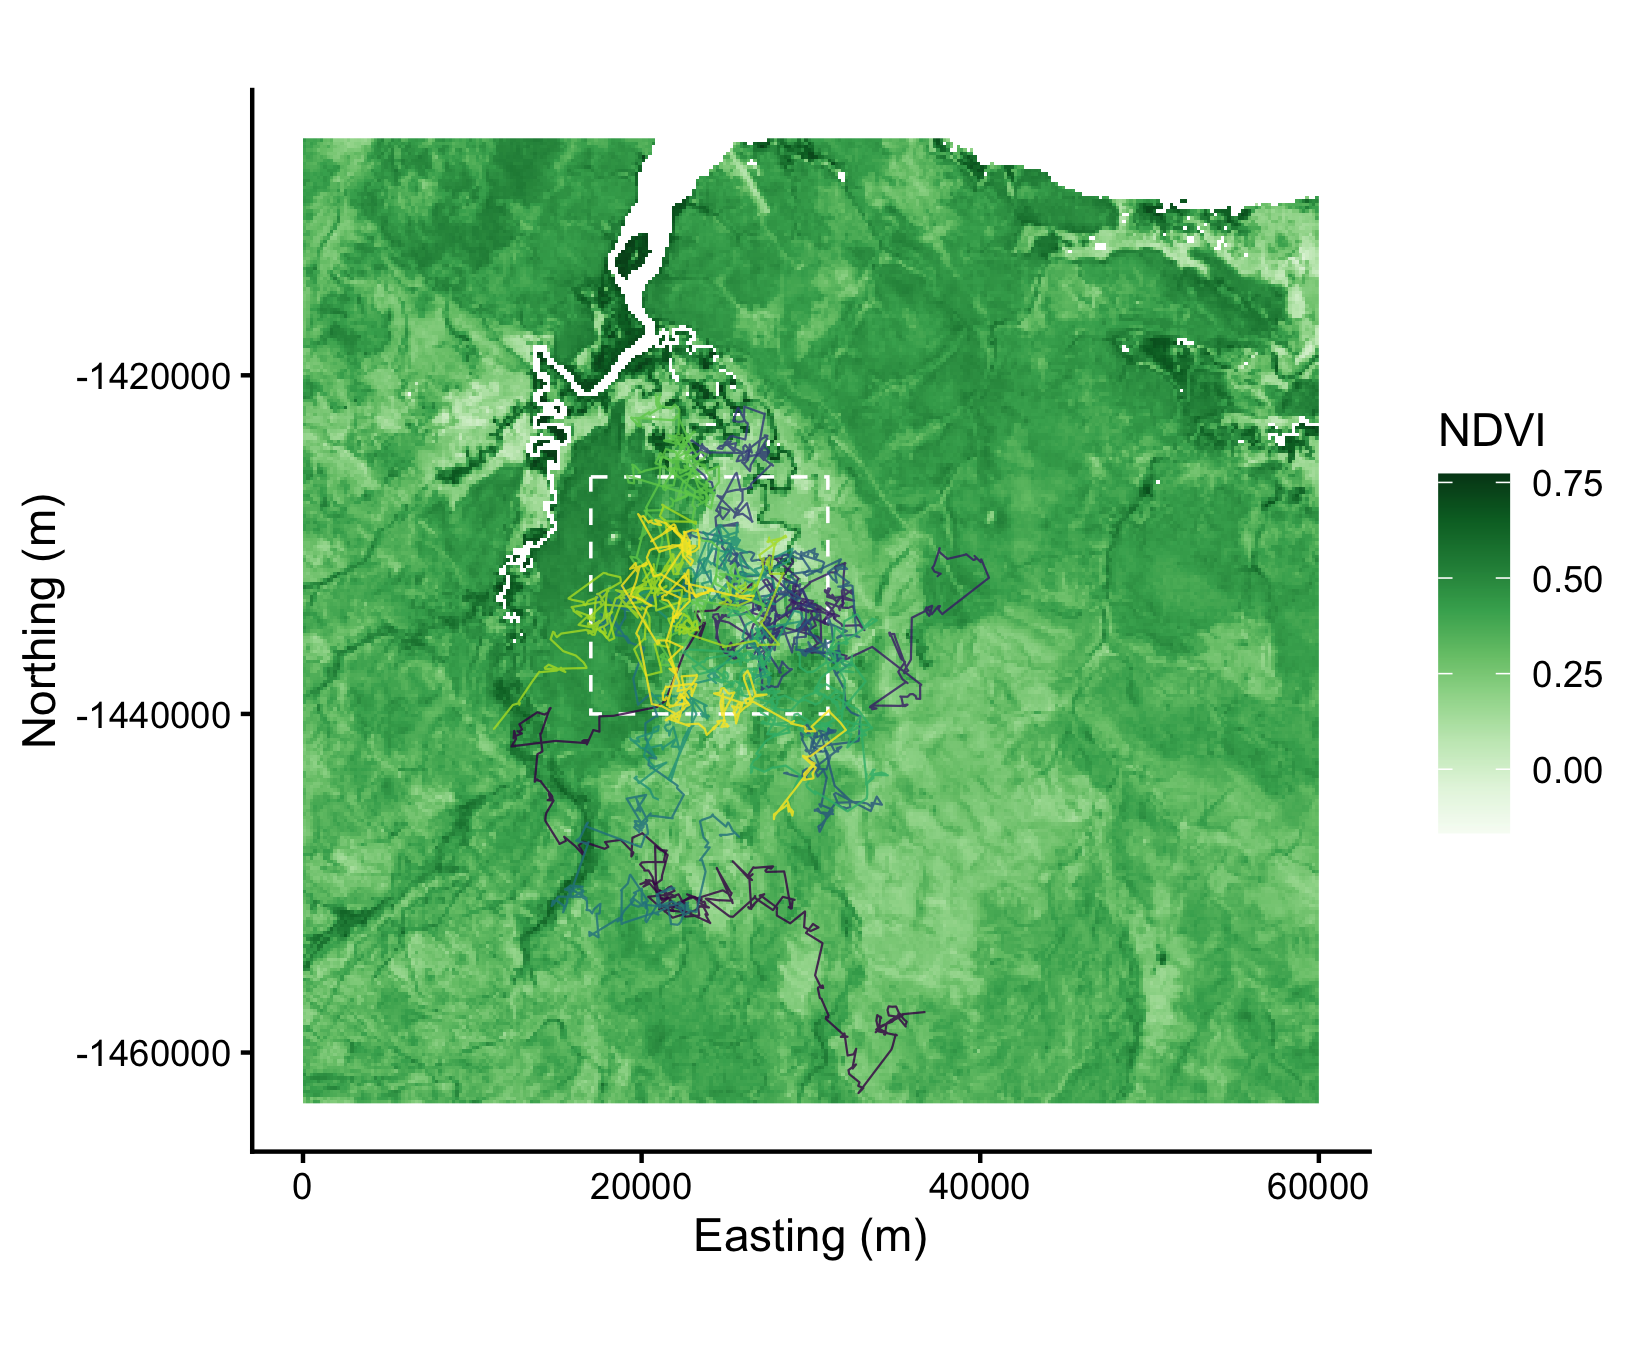
\includegraphics[keepaspectratio]{predictive_SSF_walkthrough_files/figure-pdf/amt_comparison-1.png}}

}

\caption{Paths simulated with \texttt{amt::simulate\_path()} from the
static model, over the full landscape. The dashed box is the extent used
for our own simulations.}

\end{figure}%

\subsection{Why we wrote the sampler by
hand}\label{why-we-wrote-the-sampler-by-hand}

\texttt{amt::redistribution\_kernel()} builds its kernel from
\textbf{one} fitted model evaluated against a \textbf{fixed} map. That
is exactly right for a static model, and it is the tool to reach for in
that case. Our dynamic model, though, has coefficients that change every
hour --- so there is no single set of coefficients, and no single
habitat surface, to hand it.

The custom \texttt{fun} above is most of the way to a solution. Since it
receives the proposed steps, including their timestamps, it can select
the layer matching the hour rather than using a fixed map:

\begin{Shaded}
\begin{Highlighting}[]
\CommentTok{\# Sketch: an extraction function that indexes the 24{-}layer stack of hourly}
\CommentTok{\# selection surfaces by the hour of the proposed step. Because the surfaces}
\CommentTok{\# already contain the linear predictor, the model passed to the kernel would be}
\CommentTok{\# one whose single habitat covariate is \textasciigrave{}selection\textasciigrave{}, with a coefficient of 1.}
\NormalTok{hourly\_extract }\OtherTok{\textless{}{-}} \ControlFlowTok{function}\NormalTok{(xy, map) \{}
\NormalTok{  h }\OtherTok{\textless{}{-}}\NormalTok{ lubridate}\SpecialCharTok{::}\FunctionTok{hour}\NormalTok{(xy}\SpecialCharTok{$}\NormalTok{t\_)}
\NormalTok{  xy }\SpecialCharTok{\%\textgreater{}\%}
    \FunctionTok{mutate}\NormalTok{(}
      \AttributeTok{selection =} \FunctionTok{map\_dbl}\NormalTok{(}\FunctionTok{seq\_len}\NormalTok{(}\FunctionTok{nrow}\NormalTok{(xy)), }\ControlFlowTok{function}\NormalTok{(i) \{}
\NormalTok{        terra}\SpecialCharTok{::}\FunctionTok{extract}\NormalTok{(map[[h[i] }\SpecialCharTok{+} \DecValTok{1}\NormalTok{]], }\FunctionTok{cbind}\NormalTok{(xy}\SpecialCharTok{$}\NormalTok{x\_[i], xy}\SpecialCharTok{$}\NormalTok{y\_[i]))[, }\DecValTok{1}\NormalTok{]}
\NormalTok{      \}),}
      \AttributeTok{log\_sl\_ =} \FunctionTok{log}\NormalTok{(sl\_),}
      \AttributeTok{cos\_ta\_ =} \FunctionTok{cos}\NormalTok{(ta\_)}
\NormalTok{    )}
\NormalTok{\}}
\end{Highlighting}
\end{Shaded}

That works, but note what it costs: a per-row \texttt{terra::extract()}
call, which is precisely the overhead our matrix lookup in section 8 was
written to avoid. The alternative is to rebuild the kernel for each hour
and step through them.

Either approach amounts to the bookkeeping that \texttt{simulate\_ssf()}
does explicitly. For a walkthrough, doing it by hand has the advantage
that nothing is hidden --- and it generalises immediately to whatever
other kind of temporal, seasonal or individual variation you want the
coefficients to have.

\section{Summary}\label{summary}

Starting from a single animal's GPS trajectory and three environmental
layers, we:

\begin{enumerate}
\def\labelenumi{\arabic{enumi}.}
\tightlist
\item
  Generated used and available steps, and fitted \textbf{two} step
  selection functions --- a static one and a temporally dynamic GAM with
  cyclic smooths.
\item
  Reduced both models to a common representation: a table of habitat
  coefficients and corrected movement parameters for each hour of the
  day, cross-checked against \texttt{amt}.
\item
  Pre-computed hourly habitat selection surfaces and simulated
  stochastic trajectories from each model, being explicit about how the
  choice of starting location and boundary determines what question the
  simulation answers.
\item
  Aggregated those trajectories into utilisation distributions, overall
  and by hour, and checked that the number of trajectories was
  sufficient.
\item
  Compared simulated and observed hourly movement and habitat use.
\item
  Validated the predicted distributions against the observed locations,
  overall and hour by hour.
\end{enumerate}

The recurring theme is that fitting is only the beginning. A model that
fits better by AIC has not yet earned the claim that it \emph{predicts}
better --- that claim has to be tested, and simulation is what makes
testing it possible.

This example makes the point more sharply than intended, in a way worth
being explicit about.

The dynamic model was preferred by over 1,200 AIC units, reproduced the
observed daily activity cycle that the static model cannot represent at
all, and scored substantially better hour by hour. But the whole-day
comparison --- the one that looks most like a headline result --- turned
out not to be stable at this simulation scale. Five independent runs of
the same static model on the same data returned Boyce indices from −0.04
to 0.84. Whichever one you happened to render, it would have been easy
to build a tidy story around it.

Three cautions to carry away, in roughly the order they catch people
out:

\begin{itemize}
\tightlist
\item
  \textbf{Check convergence, and believe it.} These utilisation
  distributions have \emph{not} converged at 1000 trajectories, and
  nothing about the maps would have told you so.
\item
  \textbf{Check stability the expensive way.} The split-half check in
  section 11 is cheap, reassuring, and understated the true variability
  by a factor of about thirty. Re-running the whole simulation is the
  check that counts, and the cheap proxy is not a substitute for it.
\item
  \textbf{The validation has to match the claim.} A metric that pools
  over the dimension a model is built to capture cannot detect that the
  model captures it. Choose the comparison from the question, not from
  the results.
\end{itemize}

None of this argues against the temporally dynamic approach. Its
advantage is real: it is visible in the fit, in the reproduced activity
cycle, in the hourly validation, and in the \emph{average} of repeated
whole-day comparisons. What the example argues is that a simulation
study needs the same scepticism applied to its outputs that was applied
to its inputs --- because a simulated prediction will always produce a
number, whether or not that number means anything.

\subsection{References}\label{references}

\protect\phantomsection\label{refs}
\begin{CSLReferences}{1}{1}
\bibitem[\citeproctext]{ref-Avgar2016-pb}
Avgar, Tal, Jonathan R Potts, Mark A Lewis, and Mark Boyce. 2016.
{``{Integrated step selection analysis: bridging the gap between
resource selection and animal movement}.''} \emph{Methods in Ecology and
Evolution} 7 (May): 619--30.
\url{https://doi.org/10.1111/2041-210x.12528}.

\bibitem[\citeproctext]{ref-Boyce2002-xr}
Boyce, Mark, Pierre R Vernier, Scott E Nielsen, and Fiona K A
Schmiegelow. 2002. {``{Evaluating resource selection functions}.''}
\emph{Ecological Modelling} 157 (November): 281--300.
\url{https://doi.org/10.1016/S0304-3800(02)00200-4}.

\bibitem[\citeproctext]{ref-Fieberg2021-wx}
Fieberg, John, Johannes Signer, Brian Smith, and Tal Avgar. 2021. {``{A
'How to' guide for interpreting parameters in habitat-selection
analyses}.''} \emph{The Journal of Animal Ecology} 90 (May): 1027--43.
\url{https://doi.org/10.1111/1365-2656.13441}.

\bibitem[\citeproctext]{ref-Forrest2025-le}
Forrest, Scott W, Dan Pagendam, Michael Bode, et al. 2025.
{``{Predicting fine‐scale distributions and emergent spatiotemporal
patterns from temporally dynamic step selection simulations}.''}
\emph{Ecography} 2025 (February).
\url{https://doi.org/10.1111/ecog.07421}.

\bibitem[\citeproctext]{ref-Hirzel2006-hu}
Hirzel, Alexandre H, Gwenaëlle Le Lay, Véronique Helfer, Christophe
Randin, and Antoine Guisan. 2006. {``{Evaluating the ability of habitat
suitability models to predict species presences}.''} \emph{Ecological
Modelling} 199 (November): 142--52.
\url{https://doi.org/10.1016/j.ecolmodel.2006.05.017}.

\bibitem[\citeproctext]{ref-Klappstein2024-ax}
Klappstein, Natasha J, Théo Michelot, John Fieberg, Eric J Pedersen, and
Joanna Mills Flemming. 2024. {``{Step selection functions with
non‐linear and random effects}.''} \emph{Methods in Ecology and
Evolution}, ahead of print, June 24.
\url{https://doi.org/10.1111/2041-210x.14367}.

\bibitem[\citeproctext]{ref-Signer2023-wm}
Signer, J, J Fieberg, B Reineking, et al. 2023. {``{Simulating animal
space use from fitted integrated Step‐Selection Functions (iSSF)}.''}
\emph{Methods in Ecology and Evolution}, ahead of print, December 8.
\url{https://doi.org/10.1111/2041-210x.14263}.

\bibitem[\citeproctext]{ref-Signer2019-fi}
Signer, Johannes, John Fieberg, and Tal Avgar. 2019. {``{Animal movement
tools (amt): R package for managing tracking data and conducting habitat
selection analyses}.''} \emph{Ecology and Evolution} 9 (January):
880--90. \url{https://doi.org/10.1002/ece3.4823}.

\end{CSLReferences}

\subsection{Session info}\label{session-info}

\begin{Shaded}
\begin{Highlighting}[]
\FunctionTok{sessionInfo}\NormalTok{()}
\end{Highlighting}
\end{Shaded}

\begin{verbatim}
R version 4.5.0 (2025-04-11)
Platform: aarch64-apple-darwin20
Running under: macOS 26.5.2

Matrix products: default
BLAS:   /Library/Frameworks/R.framework/Versions/4.5-arm64/Resources/lib/libRblas.0.dylib 
LAPACK: /Library/Frameworks/R.framework/Versions/4.5-arm64/Resources/lib/libRlapack.dylib;  LAPACK version 3.12.1

locale:
[1] en_US.UTF-8/en_US.UTF-8/en_US.UTF-8/C/en_US.UTF-8/en_US.UTF-8

time zone: Australia/Brisbane
tzcode source: internal

attached base packages:
[1] stats     graphics  grDevices utils     datasets  methods   base     

other attached packages:
 [1] magick_2.9.1       tictoc_1.2.1       patchwork_1.3.2    viridis_0.6.5     
 [5] viridisLite_0.4.3  RColorBrewer_1.1-3 gratia_0.10.0      mgcv_1.9-4        
 [9] nlme_3.1-168       terra_1.9-34       sf_1.1-2           amt_0.3.1.0       
[13] lubridate_1.9.5    forcats_1.0.0      stringr_1.5.2      dplyr_1.2.1       
[17] purrr_1.2.2        readr_2.1.5        tidyr_1.3.1        tibble_3.3.1      
[21] ggplot2_4.0.3      tidyverse_2.0.0   

loaded via a namespace (and not attached):
 [1] tidyselect_1.2.1   farver_2.1.2       S7_0.2.2           fastmap_1.2.0     
 [5] digest_0.6.37      timechange_0.4.0   lifecycle_1.0.5    survival_3.8-3    
 [9] magrittr_2.0.5     compiler_4.5.0     rlang_1.3.0        tools_4.5.0       
[13] utf8_1.2.6         yaml_2.3.12        data.table_1.17.0  knitr_1.51        
[17] labeling_0.4.3     fitdistrplus_1.2-2 bit_4.6.0          classInt_0.4-11   
[21] KernSmooth_2.23-26 withr_3.0.3        grid_4.5.0         e1071_1.7-17      
[25] iterators_1.0.14   scales_1.4.0       MASS_7.3-65        dichromat_2.0-0.1 
[29] mvtnorm_1.3-3      cli_3.6.6          rmarkdown_2.29     crayon_1.5.3      
[33] generics_0.1.4     rstudioapi_0.17.1  tzdb_0.5.0         DBI_1.3.0         
[37] proxy_0.4-29       splines_4.5.0      parallel_4.5.0     vctrs_0.7.3       
[41] boot_1.3-31        Matrix_1.7-3       jsonlite_2.0.0     hms_1.1.4         
[45] ecospat_4.1.2      bit64_4.8.4        foreach_1.5.2      units_1.0-1       
[49] glue_1.8.1         ggokabeito_0.1.0   codetools_0.2-20   mvnfast_0.2.8     
[53] stringi_1.8.7      gtable_0.3.6       circular_0.5-1     pillar_1.11.1     
[57] htmltools_0.5.8.1  R6_2.6.1           Rdpack_2.6.4       vroom_1.7.1       
[61] evaluate_1.0.5     lattice_0.22-6     rbibutils_2.3      backports_1.5.0   
[65] class_7.3-23       Rcpp_1.1.2         gridExtra_2.3      checkmate_2.3.2   
[69] xfun_0.57          pkgconfig_2.0.3   
\end{verbatim}




\end{document}
